% Finished mode.
% \documentclass[nocolor]{article}
% \documentclass{article}

% Draft mode.
% \documentclass[working,nocolor]{article}
\documentclass[working]{article}

%%%%%%%%%%%%%%%%%%%%%%%%%%%%%%%%%%%%%%%%%%%%%%%%%%%%%%%%%%%%%%%%%%%%%%%%%%%%%%%
%                                Basic Packages                               %
%%%%%%%%%%%%%%%%%%%%%%%%%%%%%%%%%%%%%%%%%%%%%%%%%%%%%%%%%%%%%%%%%%%%%%%%%%%%%%%

% Gives us multiple colors.
\usepackage[usenames,dvipsnames,pdftex]{xcolor}
% Lets us style link colors.
\usepackage{hyperref}
% Lets us import images and graphics.
\usepackage{graphicx}
% Lets us use figures in floating environments.
\usepackage{float}
% Lets us create multiple columns.
\usepackage{multicol}
% Gives us better math syntax.
\usepackage{amsmath,amsfonts,mathtools,amsthm,amssymb}
% Lets us strikethrough text.
\usepackage{cancel}
% Lets us edit the caption of a figure.
\usepackage{caption}
% Lets us import pdf directly in our tex code.
\usepackage{pdfpages}
% Lets us do algorithm stuff.
\usepackage[ruled,vlined,linesnumbered]{algorithm2e}
% Use a smiley face for our qed symbol.
\usepackage{tikzsymbols}
\renewcommand\qedsymbol{$\Laughey$}

\def\class{article}


%%%%%%%%%%%%%%%%%%%%%%%%%%%%%%%%%%%%%%%%%%%%%%%%%%%%%%%%%%%%%%%%%%%%%%%%%%%%%%%
%                                Basic Settings                               %
%%%%%%%%%%%%%%%%%%%%%%%%%%%%%%%%%%%%%%%%%%%%%%%%%%%%%%%%%%%%%%%%%%%%%%%%%%%%%%%

%%%%%%%%%%%%%
%  Symbols  %
%%%%%%%%%%%%%

\let\implies\Rightarrow
\let\impliedby\Leftarrow
\let\iff\Leftrightarrow
\let\epsilon\varepsilon


% KL divergence
\DeclarePairedDelimiterX{\infdivx}[2]{(}{)}{%
  #1\;\delimsize\|\;#2%
}
\newcommand{\infdiv}{D_{\mathbb{KL}}\infdivx}
\DeclarePairedDelimiter{\norm}{\lVert}{\rVert}

% argmin max
\DeclareMathOperator*{\argmax}{\arg\!max}
\DeclareMathOperator*{\argmin}{\arg\!min}
\DeclareMathOperator*{\vperp}{\text{\rotatebox{90}{$\models$}}}



%%%%%%%%%%%%
%  Tables  %
%%%%%%%%%%%%

\setlength{\tabcolsep}{5pt}
\renewcommand\arraystretch{1.5}

%%%%%%%%%%%%%%
%  SI Unitx  %
%%%%%%%%%%%%%%

\usepackage{siunitx}
\sisetup{locale = FR}

%%%%%%%%%%
%  TikZ  %
%%%%%%%%%%

\usepackage[framemethod=TikZ]{mdframed}
\usepackage{tikz}
\usepackage{tikz-cd}
\usepackage{tikzsymbols}

\usetikzlibrary{intersections, angles, quotes, calc, positioning}
\usetikzlibrary{arrows.meta}

\tikzset{
  force/.style={thick, {Circle[length=2pt]}-stealth, shorten <=-1pt}
}

%%%%%%%%%%%%%%%
%  PGF Plots  %
%%%%%%%%%%%%%%%

\usepackage{pgfplots}
\pgfplotsset{compat=1.13}

%%%%%%%%%%%%%%%%%%%%%%%
%  Center Title Page  %
%%%%%%%%%%%%%%%%%%%%%%%

\usepackage{titling}
\renewcommand\maketitlehooka{\null\mbox{}\vfill}
\renewcommand\maketitlehookd{\vfill\null}

%%%%%%%%%%%%%%%%%%%%%%%%%%%%%%%%%%%%%%%%%%%%%%%%%%%%%%%
%  Create a grey background in the middle of the PDF  %
%%%%%%%%%%%%%%%%%%%%%%%%%%%%%%%%%%%%%%%%%%%%%%%%%%%%%%%

\usepackage{eso-pic}
\newcommand\definegraybackground{
  \definecolor{reallylightgray}{HTML}{FAFAFA}
  \AddToShipoutPicture{
    \ifthenelse{\isodd{\thepage}}{
      \AtPageLowerLeft{
        \put(\LenToUnit{\dimexpr\paperwidth-222pt},0){
          \color{reallylightgray}\rule{222pt}{297mm}
        }
      }
    }
    {
      \AtPageLowerLeft{
        \color{reallylightgray}\rule{222pt}{297mm}
      }
    }
  }
}

%%%%%%%%%%%%%%%%%%%%%%%%
%  Modify Links Color  %
%%%%%%%%%%%%%%%%%%%%%%%%

\hypersetup{
  % Enable highlighting links.
  colorlinks,
  % Change the color of links to blue.
  linkcolor=blue,
  % Change the color of citations to black.
  citecolor={black},
  % Change the color of url's to blue with some black.
  urlcolor={blue!80!black}
}

%%%%%%%%%%%%%%%%%%
% Fix WrapFigure %
%%%%%%%%%%%%%%%%%%

\newcommand{\wrapfill}{\par\ifnum\value{WF@wrappedlines}>0
    \parskip=0pt
    \addtocounter{WF@wrappedlines}{-1}%
    \null\vspace{\arabic{WF@wrappedlines}\baselineskip}%
    \WFclear
\fi}

%%%%%%%%%%%%%%%%%
% Multi Columns %
%%%%%%%%%%%%%%%%%

\let\multicolmulticols\multicols
\let\endmulticolmulticols\endmulticols

\RenewDocumentEnvironment{multicols}{mO{}}
{%
  \ifnum#1=1
    #2%
  \else % More than 1 column
    \multicolmulticols{#1}[#2]
  \fi
}
{%
  \ifnum#1=1
\else % More than 1 column
  \endmulticolmulticols
\fi
}

\newlength{\thickarrayrulewidth}
\setlength{\thickarrayrulewidth}{5\arrayrulewidth}


%%%%%%%%%%%%%%%%%%%%%%%%%%%%%%%%%%%%%%%%%%%%%%%%%%%%%%%%%%%%%%%%%%%%%%%%%%%%%%%
%                           School Specific Commands                          %
%%%%%%%%%%%%%%%%%%%%%%%%%%%%%%%%%%%%%%%%%%%%%%%%%%%%%%%%%%%%%%%%%%%%%%%%%%%%%%%

%%%%%%%%%%%%%%%%%%%%%%%%%%%
%  Initiate New Counters  %
%%%%%%%%%%%%%%%%%%%%%%%%%%%

\newcounter{lecturecounter}

%%%%%%%%%%%%%%%%%%%%%%%%%%
%  Helpful New Commands  %
%%%%%%%%%%%%%%%%%%%%%%%%%%

\makeatletter

\newcommand\resetcounters{
  % Reset the counters for subsection, subsubsection and the definition
  % all the custom environments.
  \setcounter{subsection}{0}
  \setcounter{subsubsection}{0}
  \setcounter{paragraph}{0}
  \setcounter{subparagraph}{0}
  \setcounter{theorem}{0}
  \setcounter{claim}{0}
  \setcounter{corollary}{0}
  \setcounter{lemma}{0}
  \setcounter{exercise}{0}

  \@ifclasswith\class{nocolor}{
    \setcounter{definition}{0}
  }{}
}

%%%%%%%%%%%%%%%%%%%%%
%  Lecture Command  %
%%%%%%%%%%%%%%%%%%%%%

\usepackage{xifthen}

% EXAMPLE:
% 1. \lesson{Oct 17 2022 Mon (08:46:48)}{Lecture Title}
% 2. \lesson[4]{Oct 17 2022 Mon (08:46:48)}{Lecture Title}
% 3. \lesson{Oct 17 2022 Mon (08:46:48)}{}
% 4. \lesson[4]{Oct 17 2022 Mon (08:46:48)}{}
% Parameters:
% 1. (Optional) Lesson number.
% 2. Time and date of lecture.
% 3. Lecture Title.
\def\@lesson{}
\newcommand\lesson[3][\arabic{lecturecounter}]{
  % Add 1 to the lecture counter.
  \addtocounter{lecturecounter}{1}

  % Set the section number to the lecture counter.
  \setcounter{section}{#1}
  \renewcommand\thesubsection{#1.\arabic{subsection}}

  % Reset the counters.
  \resetcounters

  % Check if user passed the lecture title or not.
  \ifthenelse{\isempty{#3}}{
    \def\@lesson{Lecture \arabic{lecturecounter}}
  }{
    \def\@lesson{Lecture \arabic{lecturecounter}: #3}
  }

  % Display the information like the following:
  %                                                  Oct 17 2022 Mon (08:49:10)
  % ---------------------------------------------------------------------------
  % Lecture 1: Lecture Title
  \hfill\small{#2}
  \hrule
  \vspace*{-0.3cm}
  \section*{\@lesson}
  \addcontentsline{toc}{section}{\@lesson}
}

%%%%%%%%%%%%%%%%%%%%
%  Import Figures  %
%%%%%%%%%%%%%%%%%%%%

\usepackage{import}
\pdfminorversion=7

% EXAMPLE:
% 1. \incfig{limit-graph}
% 2. \incfig[0.4]{limit-graph}
% Parameters:
% 1. The figure name. It should be located in figures/NAME.tex_pdf.
% 2. (Optional) The width of the figure. Example: 0.5, 0.35.
\newcommand\incfig[2][1]{%
  \def\svgwidth{#1\columnwidth}
  \import{./figures/}{#2.pdf_tex}
}

\begingroup\expandafter\expandafter\expandafter\endgroup
\expandafter\ifx\csname pdfsuppresswarningpagegroup\endcsname\relax
\else
  \pdfsuppresswarningpagegroup=1\relax
\fi

%%%%%%%%%%%%%%%%%
% Fancy Headers %
%%%%%%%%%%%%%%%%%

\usepackage{fancyhdr}

% Force a new page.
\newcommand\forcenewpage{\clearpage\mbox{~}\clearpage\newpage}

% This command makes it easier to manage my headers and footers.
\newcommand\createintro{
  % Use roman page numbers (e.g. i, v, vi, x, ...)
  \pagenumbering{roman}

  % Display the page style.
  \maketitle
  % Make the title pagestyle empty, meaning no fancy headers and footers.
  \thispagestyle{empty}
  % Create a newpage.
  \newpage

  % Input the intro.tex page if it exists.
  \IfFileExists{intro.tex}{ % If the intro.tex file exists.
    % Input the intro.tex file.
    Lecture notes from the postgraduate course STAT5010, given by professor
Tony SIT at the Department of Statistics at CUHK in the academic year 2022-23. This
course covers \textit{Point Estimation} and \textit{Hypothesis Testing} mainly. 
Credit for the material in these notes is due to professor
SIT, while the structure is loosely taken from the professor released handwriting notes. 
The credit for the typesetting is my own.

\textit{Disclaimer:} This document will inevitably contain some mistakes — both
simple typos and legitimate errors. Keep in mind that these are the notes of an
postgraduate student in the process of learning the material himself, so take
what you read with a grain of salt. If you find mistakes and feel like telling
me, I will be grateful and happy to hear from you, even for the most trivial of
errors. You can reach me by email, in English or Chinese, at
\href{mailto:xcchow@126.com}{xcchow@126.com}.

    % Make the pagestyle fancy for the intro.tex page.
    \pagestyle{fancy}

    % Remove the line for the header.
    \renewcommand\headrulewidth{0pt}

    % Remove all header stuff.
    \fancyhead{}

    % Add stuff for the footer in the center.
    \fancyfoot[C]{
      % \textit{For more notes like this, visit
      % \href{\linktootherpages}{\shortlinkname}}. \\
      \vspace{0.1cm}
      \hrule
      \vspace{0.1cm}
      \@author, \\
      \term: \academicyear, \\
      Last Update: \@date, \\
      \faculty
    }
  }{ % If the intro.tex file doesn't exist.
    % Force a \newpageage.
    \forcenewpage
  }

  % Create a new page.
  \newpage

  % Remove the center stuff we did above, and replace it with just the page
  % number, which is still in roman numerals.
  \fancyfoot[C]{\thepage}
  % Add the table of contents.
  \tableofcontents
  % Force a new page.
  \forcenewpage

  % Move the page numberings back to arabic, from roman numerals.
  \pagenumbering{arabic}
  % Set the page number to 1.
  \setcounter{page}{1}

  % Add the header line back.
  \renewcommand\headrulewidth{0.4pt}
  % In the top right, add the lecture title.
  \fancyhead[R]{\@lesson}
  % In the top left, add the author name.
  \fancyhead[L]{\@author}
  % In the bottom center, add the page.
  \fancyfoot[C]{\thepage}
  % Add a nice gray background in the middle of all the upcoming pages.
  % \definegraybackground
}

\makeatother


%%%%%%%%%%%%%%%%%%%%%%%%%%%%%%%%%%%%%%%%%%%%%%%%%%%%%%%%%%%%%%%%%%%%%%%%%%%%%%%
%                               Custom Commands                               %
%%%%%%%%%%%%%%%%%%%%%%%%%%%%%%%%%%%%%%%%%%%%%%%%%%%%%%%%%%%%%%%%%%%%%%%%%%%%%%%

%%%%%%%%%%%%
%  Circle  %
%%%%%%%%%%%%

\newcommand*\circled[1]{\tikz[baseline=(char.base)]{
  \node[shape=circle,draw,inner sep=1pt] (char) {#1};}
}

%%%%%%%%%%%%%%%%%%%
%  Todo Commands  %
%%%%%%%%%%%%%%%%%%%

\usepackage{xargs}
\usepackage[colorinlistoftodos]{todonotes}

\makeatletter

\@ifclasswith\class{working}{
  \newcommandx\unsure[2][1=]{\todo[linecolor=red,backgroundcolor=red!25,bordercolor=red,#1]{#2}}
  \newcommandx\change[2][1=]{\todo[linecolor=blue,backgroundcolor=blue!25,bordercolor=blue,#1]{#2}}
  \newcommandx\info[2][1=]{\todo[linecolor=OliveGreen,backgroundcolor=OliveGreen!25,bordercolor=OliveGreen,#1]{#2}}
  \newcommandx\improvement[2][1=]{\todo[linecolor=Plum,backgroundcolor=Plum!25,bordercolor=Plum,#1]{#2}}

  \newcommand\listnotes{
    \newpage
    \listoftodos[Notes]
  }
}{
  \newcommandx\unsure[2][1=]{}
  \newcommandx\change[2][1=]{}
  \newcommandx\info[2][1=]{}
  \newcommandx\improvement[2][1=]{}

  \newcommand\listnotes{}
}

\makeatother

%%%%%%%%%%%%%
%  Correct  %
%%%%%%%%%%%%%

% EXAMPLE:
% 1. \correct{INCORRECT}{CORRECT}
% Parameters:
% 1. The incorrect statement.
% 2. The correct statement.
\definecolor{correct}{HTML}{009900}
\newcommand\correct[2]{{\color{red}{#1 }}\ensuremath{\to}{\color{correct}{ #2}}}


%%%%%%%%%%%%%%%%%%%%%%%%%%%%%%%%%%%%%%%%%%%%%%%%%%%%%%%%%%%%%%%%%%%%%%%%%%%%%%%
%                                 Environments                                %
%%%%%%%%%%%%%%%%%%%%%%%%%%%%%%%%%%%%%%%%%%%%%%%%%%%%%%%%%%%%%%%%%%%%%%%%%%%%%%%

\usepackage{varwidth}
\usepackage{thmtools}
\usepackage[most,many,breakable]{tcolorbox}

\tcbuselibrary{theorems,skins,hooks}
\usetikzlibrary{arrows,calc,shadows.blur}

%%%%%%%%%%%%%%%%%%%
%  Define Colors  %
%%%%%%%%%%%%%%%%%%%

\definecolor{myblue}{RGB}{45, 111, 177}
\definecolor{mygreen}{RGB}{56, 140, 70}
\definecolor{myred}{RGB}{199, 68, 64}
\definecolor{mypurple}{RGB}{197, 92, 212}

\definecolor{definition}{HTML}{228b22}
\definecolor{theorem}{HTML}{00007B}
\definecolor{example}{HTML}{2A7F7F}
\definecolor{definition}{HTML}{228b22}
\definecolor{prop}{HTML}{191971}
\definecolor{lemma}{HTML}{983b0f}
\definecolor{exercise}{HTML}{88D6D1}

\colorlet{definition}{mygreen!85!black}
\colorlet{claim}{mygreen!85!black}
\colorlet{corollary}{mypurple!85!black}
\colorlet{proof}{theorem}

%%%%%%%%%%%%%%%%%%%%%%%%%%%%%%%%%%%%%%%%%%%%%%%%%%%%%%%%%
%  Create Environments Styles Based on Given Parameter  %
%%%%%%%%%%%%%%%%%%%%%%%%%%%%%%%%%%%%%%%%%%%%%%%%%%%%%%%%%

\mdfsetup{skipabove=1em,skipbelow=0em}

%%%%%%%%%%%%%%%%%%%%%%
%  Helpful Commands  %
%%%%%%%%%%%%%%%%%%%%%%

% EXAMPLE:
% 1. \createnewtheoremstyle{thmdefinitionbox}{}{}
% 2. \createnewtheoremstyle{thmtheorembox}{}{}
% 3. \createnewtheoremstyle{thmproofbox}{qed=\qedsymbol}{
%       rightline=false, topline=false, bottomline=false
%    }
% Parameters:
% 1. Theorem name.
% 2. Any extra parameters to pass directly to declaretheoremstyle.
% 3. Any extra parameters to pass directly to mdframed.
\newcommand\createnewtheoremstyle[3]{
  \declaretheoremstyle[
  headfont=\bfseries\sffamily, bodyfont=\normalfont, #2,
  mdframed={
    #3,
  },
  ]{#1}
}

% EXAMPLE:
% 1. \createnewcoloredtheoremstyle{thmdefinitionbox}{definition}{}{}
% 2. \createnewcoloredtheoremstyle{thmexamplebox}{example}{}{
%       rightline=true, leftline=true, topline=true, bottomline=true
%     }
% 3. \createnewcoloredtheoremstyle{thmproofbox}{proof}{qed=\qedsymbol}{backgroundcolor=white}
% Parameters:
% 1. Theorem name.
% 2. Color of theorem.
% 3. Any extra parameters to pass directly to declaretheoremstyle.
% 4. Any extra parameters to pass directly to mdframed.
\newcommand\createnewcoloredtheoremstyle[4]{
  \declaretheoremstyle[
  headfont=\bfseries\sffamily\color{#2}, bodyfont=\normalfont, #3,
  mdframed={
    linewidth=2pt,
    rightline=false, leftline=true, topline=false, bottomline=false,
    linecolor=#2, backgroundcolor=#2!5, #4,
  },
  ]{#1}
}

%%%%%%%%%%%%%%%%%%%%%%%%%%%%%%%%%%%
%  Create the Environment Styles  %
%%%%%%%%%%%%%%%%%%%%%%%%%%%%%%%%%%%

\makeatletter
\@ifclasswith\class{nocolor}{
  % Environments without color.

  \createnewtheoremstyle{thmdefinitionbox}{}{}
  \createnewtheoremstyle{thmtheorembox}{}{}
  \createnewtheoremstyle{thmexamplebox}{}{}
  \createnewtheoremstyle{thmclaimbox}{}{}
  \createnewtheoremstyle{thmcorollarybox}{}{}
  \createnewtheoremstyle{thmpropbox}{}{}
  \createnewtheoremstyle{thmlemmabox}{}{}
  \createnewtheoremstyle{thmexercisebox}{}{}
  \createnewtheoremstyle{thmdefinitionbox}{}{}
  \createnewtheoremstyle{thmquestionbox}{}{}
  \createnewtheoremstyle{thmsolutionbox}{}{}

  \createnewtheoremstyle{thmproofbox}{qed=\qedsymbol}{}
  \createnewtheoremstyle{thmexplanationbox}{}{}
}{
  % Environments with color.

  \createnewcoloredtheoremstyle{thmdefinitionbox}{definition}{}{}
  \createnewcoloredtheoremstyle{thmtheorembox}{theorem}{}{}
  \createnewcoloredtheoremstyle{thmexamplebox}{example}{}{
    rightline=true, leftline=true, topline=true, bottomline=true
  }
  \createnewcoloredtheoremstyle{thmclaimbox}{claim}{}{}
  \createnewcoloredtheoremstyle{thmcorollarybox}{corollary}{}{}
  \createnewcoloredtheoremstyle{thmpropbox}{prop}{}{}
  \createnewcoloredtheoremstyle{thmlemmabox}{lemma}{}{}
  \createnewcoloredtheoremstyle{thmexercisebox}{exercise}{}{}

  \createnewcoloredtheoremstyle{thmproofbox}{proof}{qed=\qedsymbol}{backgroundcolor=white}
  \createnewcoloredtheoremstyle{thmexplanationbox}{example}{qed=\qedsymbol}{backgroundcolor=white}
}
\makeatother

%%%%%%%%%%%%%%%%%%%%%%%%%%%%%
%  Create the Environments  %
%%%%%%%%%%%%%%%%%%%%%%%%%%%%%

\declaretheorem[numberwithin=section, style=thmtheorembox,     name=Theorem]{theorem}
\declaretheorem[numbered=no,          style=thmexamplebox,     name=Example]{example}
\declaretheorem[numberwithin=section, style=thmclaimbox,       name=Claim]{claim}
\declaretheorem[numberwithin=section, style=thmcorollarybox,   name=Corollary]{corollary}
\declaretheorem[numberwithin=section, style=thmpropbox,        name=Proposition]{prop}
\declaretheorem[numberwithin=section, style=thmlemmabox,       name=Lemma]{lemma}
\declaretheorem[numberwithin=section, style=thmexercisebox,    name=Exercise]{exercise}
\declaretheorem[numbered=no,          style=thmproofbox,       name=Proof]{replacementproof}
\declaretheorem[numbered=no,          style=thmexplanationbox, name=Proof]{expl}

\makeatletter
\@ifclasswith\class{nocolor}{
  % Environments without color.

  \newtheorem*{note}{Note}

  \declaretheorem[numberwithin=section, style=thmdefinitionbox, name=Definition]{definition}
  \declaretheorem[numberwithin=section, style=thmquestionbox,   name=Question]{question}
  \declaretheorem[numberwithin=section, style=thmsolutionbox,   name=Solution]{solution}
}{
  % Environments with color.

  \newtcbtheorem[number within=section]{Definition}{Definition}{
    enhanced,
    before skip=2mm,
    after skip=2mm,
    colback=red!5,
    colframe=red!80!black,
    colbacktitle=red!75!black,
    boxrule=0.5mm,
    attach boxed title to top left={
      xshift=1cm,
      yshift*=1mm-\tcboxedtitleheight
    },
    varwidth boxed title*=-3cm,
    boxed title style={
      interior engine=empty,
      frame code={
        \path[fill=tcbcolback]
        ([yshift=-1mm,xshift=-1mm]frame.north west)
        arc[start angle=0,end angle=180,radius=1mm]
        ([yshift=-1mm,xshift=1mm]frame.north east)
        arc[start angle=180,end angle=0,radius=1mm];
        \path[left color=tcbcolback!60!black,right color=tcbcolback!60!black,
        middle color=tcbcolback!80!black]
        ([xshift=-2mm]frame.north west) -- ([xshift=2mm]frame.north east)
        [rounded corners=1mm]-- ([xshift=1mm,yshift=-1mm]frame.north east)
        -- (frame.south east) -- (frame.south west)
        -- ([xshift=-1mm,yshift=-1mm]frame.north west)
        [sharp corners]-- cycle;
      },
    },
    fonttitle=\bfseries,
    title={#2},
    #1
  }{def}

  \NewDocumentEnvironment{definition}{O{}O{}}
    {\begin{Definition}{#1}{#2}}{\end{Definition}}

  \newtcolorbox{note}[1][]{%
    enhanced jigsaw,
    colback=gray!20!white,%
    colframe=gray!80!black,
    size=small,
    boxrule=1pt,
    title=\textbf{Note:-},
    halign title=flush center,
    coltitle=black,
    breakable,
    drop shadow=black!50!white,
    attach boxed title to top left={xshift=1cm,yshift=-\tcboxedtitleheight/2,yshifttext=-\tcboxedtitleheight/2},
    minipage boxed title=1.5cm,
    boxed title style={%
      colback=white,
      size=fbox,
      boxrule=1pt,
      boxsep=2pt,
      underlay={%
        \coordinate (dotA) at ($(interior.west) + (-0.5pt,0)$);
        \coordinate (dotB) at ($(interior.east) + (0.5pt,0)$);
        \begin{scope}
          \clip (interior.north west) rectangle ([xshift=3ex]interior.east);
          \filldraw [white, blur shadow={shadow opacity=60, shadow yshift=-.75ex}, rounded corners=2pt] (interior.north west) rectangle (interior.south east);
        \end{scope}
        \begin{scope}[gray!80!black]
          \fill (dotA) circle (2pt);
          \fill (dotB) circle (2pt);
        \end{scope}
      },
    },
    #1,
  }

  \newtcbtheorem{Question}{Question}{enhanced,
    breakable,
    colback=white,
    colframe=myblue!80!black,
    attach boxed title to top left={yshift*=-\tcboxedtitleheight},
    fonttitle=\bfseries,
    title=\textbf{Question:-},
    boxed title size=title,
    boxed title style={%
      sharp corners,
      rounded corners=northwest,
      colback=tcbcolframe,
      boxrule=0pt,
    },
    underlay boxed title={%
      \path[fill=tcbcolframe] (title.south west)--(title.south east)
      to[out=0, in=180] ([xshift=5mm]title.east)--
      (title.center-|frame.east)
      [rounded corners=\kvtcb@arc] |-
      (frame.north) -| cycle;
    },
    #1
  }{def}

  \NewDocumentEnvironment{question}{O{}O{}}
  {\begin{Question}{#1}{#2}}{\end{Question}}

  \newtcolorbox{Solution}{enhanced,
    breakable,
    colback=white,
    colframe=mygreen!80!black,
    attach boxed title to top left={yshift*=-\tcboxedtitleheight},
    title=\textbf{Solution:-},
    boxed title size=title,
    boxed title style={%
      sharp corners,
      rounded corners=northwest,
      colback=tcbcolframe,
      boxrule=0pt,
    },
    underlay boxed title={%
      \path[fill=tcbcolframe] (title.south west)--(title.south east)
      to[out=0, in=180] ([xshift=5mm]title.east)--
      (title.center-|frame.east)
      [rounded corners=\kvtcb@arc] |-
      (frame.north) -| cycle;
    },
  }

  \NewDocumentEnvironment{solution}{O{}O{}}
  {\vspace{-10pt}\begin{Solution}{#1}{#2}}{\end{Solution}}
}
\makeatother

%%%%%%%%%%%%%%%%%%%%%%%%%%%%
%  Edit Proof Environment  %
%%%%%%%%%%%%%%%%%%%%%%%%%%%%

\renewenvironment{proof}[1][\proofname]{\vspace{-10pt}\begin{replacementproof}}{\end{replacementproof}}
\newenvironment{explanation}[1][\proofname]{\vspace{-10pt}\begin{expl}}{\end{expl}}

\theoremstyle{definition}

\newtheorem*{notation}{Notation}
\newtheorem*{previouslyseen}{As previously seen}
\newtheorem*{problem}{Problem}
\newtheorem*{observe}{Observe}
\newtheorem*{property}{Property}
\newtheorem*{intuition}{Intuition}

% \usepackage{lipsum} % For random text. You don't need this.
\usepackage{enumerate}
\usepackage{natbib}
\bibliographystyle{abbrvnat}
\setcitestyle{authoryear, open={(},close={)}}
\usepackage{booktabs}
\usepackage{multirow}

\title{STAT5010 Lecture Notes (Remake)}
\author{Xiaocheng Zhou}
\date{\today}

\newcommand{\linktootherpages}{link}
\newcommand{\shortlinkname}{link}
\newcommand{\term}{Fall Term}
\newcommand{\academicyear}{$2022$}
\newcommand{\faculty}{Department of Statistics}

\begin{document}
  \createintro

  % start lectures
  % \lesson{Oct 17 2022 Mon (12:28:10)}{Lecture Title}

\subsection{Sub Section 1}
\label{sub_sec:sub_section_1}

\begin{theorem}
This is a theorem.
\end{theorem}
\begin{proof}
This is a proof.
\end{proof}
\begin{example}
This is an example.
\end{example}
\begin{explanation}
This is an explanation.
\end{explanation}
\begin{claim}
This is a claim.
\end{claim}
\begin{corollary}
This is a corollary.
\end{corollary}
\begin{prop}
This is a proposition.
\end{prop}
\begin{lemma}
This is a lemma.
\end{lemma}
\begin{question}
This is a question.
\end{question}
\begin{solution}
This is a solution.
\end{solution}
\begin{exercise}
This is an exercise.
\end{exercise}
\begin{definition}[Definition]
This is a definition.
\end{definition}
\begin{note}
This is a note.
\end{note}

% subsection sub_section_1 (end)

\newpage
  % 
\lesson{Oct 19 2022 Wen (12:28:10)}{Lecture Title}

\subsection{Sub Section 2}
\label{sub_sec:sub_section_2}

\begin{theorem}
This is a theorem.
\end{theorem}
\begin{proof}
This is a proof.
\end{proof}
\begin{example}
This is an example.
\end{example}
\begin{explanation}
This is an explanation.
\end{explanation}
\begin{claim}
This is a claim.
\end{claim}
\begin{corollary}
This is a corollary.
\end{corollary}
\begin{prop}
This is a proposition.
\end{prop}
\begin{lemma}
This is a lemma.
\end{lemma}
\begin{question}
This is a question.
\end{question}
\begin{solution}
This is a solution.
\end{solution}
\begin{exercise}
This is an exercise.
\end{exercise}
\begin{definition}[Definition]
This is a definition.
\end{definition}
\begin{note}
This is a note.
\end{note}

% subsection sub_section_2 (end)

\newpage
  % \lesson{Oct 17 2022 Mon (13:18:57)}{Todo Notes}

\todo[inline]{The original todo note withouth changed colours.\newline Here's another line.}
\lipsum[11]\unsure{Is this correct?}\unsure{I'm unsure about also!}
\lipsum[11]\change{Change this!}
\lipsum[11]\info{This can help me in chapter seven!}
\lipsum[11]\improvement{This really needs to be improved!\\What was I thinking?!}
\lipsum[11]\improvement[inline]{The following section needs to be rewritten!}
\lipsum[11]

\newpage

\lesson{Oct 20 2022 Thu (12:28:10)}{Graphs}

\noindent \begin{minipage}{0.53\textwidth}
    Lorem ipsum dolor sit amet, consetetur sadipscing elitr, sed diam nonumy eirmod
    tempor invidunt ut labore et dolore magna aliquyam erat, sed diam voluptua. At
    vero eos et accusam et justo duo dolores et ea rebum. Stet clita kasd gubergren,
    no sea takimata sanctus est Lorem ipsum dolor sit amet. Lorem ipsum dolor sit
    amet, consetetur sadipscing elitr, sed diam nonumy eirmod tempor invidunt ut
    labore et dolore magna aliquyam erat, sed diam voluptua. At vero eos et accusam
    et justo duo dolores et ea rebum. Stet clita kasd gubergren, no sea takimata
    sanctus est Lorem ipsum dolor sit amet.
\end{minipage}
\hspace{0.05\textwidth}
\begin{minipage}{0.4\textwidth}
  \vspace{1cm}
  \centering
  \incfig{limit-graph}
  \captionof{figure}{$y = g(t)$}
  \label{fig:limit_graph}
\end{minipage}

\newpage
  % end lectures
  \lesson{original Lecture 1 -- 3}{Overview of Statistical Inference}

Different disciplines require to convert data to 
inference/conclusion via statistics:
\begin{itemize}
    \item genetic, medical, earth sciences
    \item economics, finance
    \item networks, images, recordings
\end{itemize}
$~$\\
% \\ \hspace*{\fill} \\
Questions concerned:
\begin{itemize}
    \item capture the uncertainty. {\color{gray}signal+noises}
    \item methodology
    \begin{itemize}
        \item point estimator 
        {\color{gray}e.g. 
        $\hat{\beta}=
        (\boldsymbol{X}^T\boldsymbol{X})^{-1}\boldsymbol{X}^T\boldsymbol{y}$, where $\boldsymbol{y}$ is r.v..
        }
        \item testing $\sim$ confidence region
        {\color{gray} e.g.
        $H_0:~\theta=\theta_0$ vs $H_1:~\theta=\theta_1$
        }
    \end{itemize}
    \item optimality / optimal inference
    \begin{itemize}
        \item finite-sample optimality 
        {\color{gray}
        iid obs: $x_1,\cdots,x_n$
        }
        \item asymptotic properties 
        {\color{gray} 
        $n\to\infty$
        }
    \end{itemize}
\end{itemize}

\subsection{Decision Theory }%\citep{Wald1939}}

\begin{gather}
    (X_1,\cdots,X_n)\overset{iid}{\sim}F~(\text{or}~f)
\end{gather}
A statistical model is a family of distributions $\mathbb{P}$ indexed by
a parameter $\theta$. We demote
\begin{gather}
    \mathbb{P}=\{p_\theta:~\theta\in\Omega\}
\end{gather}
where $\Omega\in\mathbb{R}^k$ is parameter space.

\begin{example}
    Flipping a coin.\\
    
    obs (data): a sequence of coin flips $(X_1,\cdots,X_n)$. 
    One can write $\mathbb{P}=\{\text{Bernoulli}(\theta): \theta\in[0,1]\triangleq\Omega\}$ and $P_\theta(X_i=1)=\theta$\\
    
    data $\boldsymbol{X}$\\
    $\Rightarrow$ estimator: $\hat{\theta}(\boldsymbol{X})$ for the parameter $h(\theta)$ 
    {\color{gray} e.g. ($\bar{X}=\frac{1}{n}\sum_{i=1}^nX_i$)}\\
    $\Rightarrow$ $\hat{\theta}(\boldsymbol{X})$ for estimation and testing.
\end{example}

\subsubsection{A Decision Procedure}
\begin{definition}[Estimator]
    $\delta:\mathcal{X}\to\mathcal{D}$, 
    a map from sample space $\mathcal{X}$ to decision space $\mathcal{D}$.
\end{definition}

\begin{example}
    Take $\mathbb{P}=\{\text{Bernoulli}(\theta)\}$ as shown earlier,
    \begin{enumerate}
        \item \textbf{Estimating $\theta$:} 
        the dicision space is $\mathcal{D}=[0,1]$ and 
        one possible decision procedure can be 
        $\delta(\boldsymbol{X})=\bar{X}_n$.
        \item \textbf{Hypothesis testing:} 
        Accept/Reject the Null hypothesis $H_0:\theta=\frac{1}{2}$. 
        Correspondingly, the decision space is $\mathcal{D}=\{\text{Accept, Reject}\}$.
        One possible procedure is $\delta(\boldsymbol{X})=$
        \textit{``Reject to if $\bar{X}_n > 0.5$ and accept it otherwise''}.
        \item A loss function is mapping $L: \Omega\times\mathcal{D} \to \mathbb{R}^+\cup{\{0\}}$.
        $L(\theta, d)$  represents the penalty for making the decision $d$ 
        when $\theta$ is in fact the true parameter for the distribution generating the data.
    \end{enumerate}
\end{example}

Loss function
\begin{itemize}
    \item Squared error loss: $L(\theta,d)=(\theta-d)^2$
    \item Abstract error loss: $L(\theta,d)=|\theta-d|$
    \item Risk function: 
    $L(\theta,d)=\int{\omega(\theta)(\theta-d)^2d\Lambda(\theta)}$
\end{itemize}

Frequentist perspective: $\theta$ is fixed yet unknown;
Bayesian perspective: $\Theta\sim$ distribution.

\begin{definition}[Risk function]
    Overall weighted average of $L(\theta,\delta)$
    \begin{gather}
        R(\theta, \delta)=\mathbb{E}_\theta L(\theta, \delta(\boldsymbol{X}))
    \end{gather}
\end{definition}

\begin{definition}[Admissibility]
\label{def:admissible}
    $\delta$ is inadmissible if there exists $\delta'$ such that 
    \begin{enumerate}[{(1)}]
        \item $R(\theta, \delta') \leq R(\theta, \delta)~\forall{\theta}\in\Omega$ and 
        \item $R(\theta', \delta') < R(\theta', \delta)~\text{for some}~\theta'\in\Omega$
    \end{enumerate}
    Otherwise, the $\delta$ is admissible.
\end{definition}
\info{\scriptsize
You should be superior to any other applicant in at least one aspect, 
or you will not be admitted.}

\subsubsection{Types of Model}
\begin{enumerate}
    \item Parametric models: Bernoulli($\theta$), $\mathcal{N}(\mu,\sigma^2)$, t($k$), ...
    \item Non-parametric models: empirical cdf $\hat{F}_n(x)=\frac{1}{n}\sum_{i=1}^n{I(X_i\leq{x})}$
    \item Semi-parametric models: Cox proportional hazard model
    % \begin{align}
    %     \lambda(t|Z(t))&=\lambda_0(t)\exp{(\beta^TZ(t))}
    %     &=\frac{f(t|Z)}{}
        
    % \end{align}
\end{enumerate}


\subsection{Large-Sample Theory}
\subsubsection{Convergence in probability}
\begin{definition}[Convergence in probability]
    A sequence of random variable $Y_n$ (e.g. $\delta_n(\boldsymbol{X})=\frac{1}{n}\sum_{i=1}^n{X_i}$) 
    converges in probability to a random variable $Y$ as $n\to\infty$,
    written as $Y_n\overset{p}{\longrightarrow}Y$,
    if $\forall{\varepsilon}>0$
    \begin{gather}
        P(|Y_n-Y|\geq \varepsilon)\overset{n\to\infty}{\longrightarrow}0
    \end{gather}
\end{definition}

\begin{example}
    \textbf{Weak Law of Large Numbers (WLLNs)}\\
    $X_1,\cdots,X_n\overset{iid}{\sim}(\mu,\sigma^2),~\sigma^2<\infty,\bar{X}_n=\frac{1}{n}\sum_{i=1}^n{X_i}$,
    $\mathbb{E}(\bar{X}_n-\mu)^2=\mathrm{Var}\bar{X}_n=\frac{\sigma^2}{n} \to 0$ as $n\to\infty$,
    in which case $\bar{X}_n\overset{p}{\longrightarrow}\mu$ as $n\to\infty$.
\end{example}

\begin{prop}
    If $f(\cdot)$ is continuous at $c$, and if $Y_n\overset{p}{\longrightarrow}c$, then $f(Y_n)\overset{p}{\longrightarrow}f(c)$.
\end{prop}
\begin{proof}
    Since $f$ is continuous at $c$, given any $\varepsilon > 0$, 
    then exists $\delta_\varepsilon > 0$ such that $|f(y)-f(c)|<\varepsilon$ 
    whenever $|y-c|<\delta_\varepsilon$. 
    Thus
    \begin{gather}
        P(|Y_n-c|<\delta_\varepsilon)\leq P(|f(y_n)-f(c)|<\varepsilon)
    \end{gather}
    which implies
    \begin{gather}
        P(|f(y_n)-f(c)|\geq\varepsilon) \leq P(|Y_n-c|>\delta_\varepsilon) \to 0
    \end{gather}
    as $Y_n\overset{p}{\longleftarrow}$ as $n\to\infty$.
\end{proof}
\info{\scriptsize $\delta-\varepsilon$ language}

\subsubsection{Convergence in distribution}
\begin{definition}[Convergence in distribution]
    A sequence of r.v.'s $Y_n~(n \geq 1)$ with cdf's $H_n$ converges
    in distribution (in law) to a random variable $Y$ with cdf $H$ if
    \begin{gather}
        H_n(y)\to H(y)
    \end{gather}
    as $n\to\infty$ whenever $H$ continuous at $y$. 
    For notation, we write $Y_n\Rightarrow Y$ or $Y_n\overset{d/l}{\longrightarrow}Y$.
\end{definition}

\begin{example}
    Suppose $Y_n=\frac{1}{n}$, a degenerate r.v. and that $Y$ is always 0.
    Then 
    \begin{gather}
        H_n(y)=P(Y_n\leq y)=\mathbb{I}(\frac{1}{n}\leq y).
    \end{gather}
    If $y>0$, then $H_n(y)=\mathbb{I}(\frac{1}{n}\leq y)\to 1$ as $n\to\infty$
    for eventually $\frac{1}{n}$ will be less than $y$.
    If $y\leq 0$, then $H_n(y)=\mathbb{I}(\frac{1}{n}\leq y)=0$ for all $n$ and 
    so $H_n(y)\to 0$ as $n\to\infty$.
    \newline
    Note that $H(y)=P(Y\leq y)=\mathbb{I}(0\leq y)$. Comparisons with
    the limits just obtained show that $H_n(y)\to H(y)$ if $y \neq 0$, 
    but $H_n(0) = 0 \to 0 \neq 1 = H(0)$. 
    So, in this example, $Y_n\overset{d}{\longrightarrow}Y$
    but the cumulative distribution function do not converge to $H(y)$ as $y=0$.
\end{example}

\newpage
  \lesson{original Lecture 3}{10 Ways of Viewing a Random Variable}
\subsection{Familiar Perspectives}

\begin{enumerate}
    \item probability space
    \item random variable
    \item distribution
    \item $\cdots$
\end{enumerate}


\begin{definition}[Probability space]
    $(\Omega,\mathcal{F},P)$, 
    where $\Omega$ is sample space with element $\omega$,
    $\Omega$ is $\sigma$-algebra/$\sigma$-field, and 
    $P$ is probability measure.
\end{definition}
\info{\scriptsize refer to Measure Theory (Probability and Measures, Billingsley, 1995)}

\subsection{Characteristic Functions (ch.f.)}

\begin{definition}[ch.f.]
    \begin{gather}
        \Phi_X(t)=\mathbb{E}(e^{itX})=\int{e^{itx}}dF(x)
    \end{gather}
    where $i=\sqrt{-1}$ and $e^{itx}=\cos{tx}+i\sin{tx}$.
\end{definition}

\begin{example}
    The characteristic function of $Z\sim{\mathcal{N}(0,1)}$:
    \begin{gather}
        \Phi_Z(t)=\exp{\{-\frac{1}{2}t^2\}}
    \end{gather}
\end{example}

\begin{align}
    |\mathbb{E}e^{itX}| 
    \leq& \mathbb{E}|e^{itX}| \\
    =& \mathbb{E}|\cos{(tX)}+i\sin{(tX)}| \\
    =& \mathbb{E}\sqrt{\cos^2(tX)+\sin^2(tX)}=1
\end{align}

Inversion formula:
\begin{align}
    f_X(x)=&\frac{1}{2\pi}\int_{-\infty}^\infty{e^{-itx}\Phi_X(t)}dt \\
    F_X(x) - F_X(y)=&\frac{1}{2\pi}\int_{-\infty}^\infty\frac{e^{-ity}-e^{-itx}}{it}\Phi_X(t)dt
\end{align}
for the continuous points of $F_X(x)$ and $F_X(y)$.

\begin{theorem}
    \textbf{Uniqueness of ch.f.}\\
    Let $X$ and $Y$ be random $k$-vectors, then
    \begin{enumerate}
        \item If $Phi_X(t)=\Phi_Y(t),~\forall{t}\in\mathbb{R}^k$, then $F_X=F_Y$;
        \item If $M_X(t)=M_Y(t)<\infty,~\forall{t}~s.t.~|t|<h$, then $F_X=F_Y$
    \end{enumerate}
\end{theorem}
\begin{proof}
$~$\\
    \begin{enumerate}
        \item \label{prf:uniqchf1} For any $\boldsymbol{a}=(a_1, \cdots, a_k)^T\in\mathbb{R}^k$, $\boldsymbol{b}\in\mathbb{R}^k$,
        and $(\boldsymbol{a},\boldsymbol{b}]=(a_1,b_1]\times\cdots\times(a_k,b_k]$
        satisfying $P_X(\text{the boundary of}~(\boldsymbol{a},\boldsymbol{b}])=0$,
        \begin{gather}
            P((\boldsymbol{a},\boldsymbol{b}])
            =\lim_{c\to\infty}\int_{-c}^c\cdots\int_{-c}^c{
            \frac{\Phi_X(t_1,\cdots,t_k)}{(-1)^{\frac{k}{2}(2\pi)^k}}
            }\prod_{j=1}^k\frac{e^{-it_ja_j}-e^{-it_jb_j}}{it_j}dt_j
        \end{gather}
        \item \label{prf:uniqchf2} First, consider the case where $k=1$. Since
        \begin{gather}
            e^{s|x|}\leq e^{sx}+e^{-sx},
        \end{gather}
        we conclude that $|X|$ has an MGF that is finite in the neighborhood $(-c,c)$ for some $c>0$,
        and that $|X|$ has finite moments of all orders.\\
        Observe that 
        \begin{gather}
            \left| e^{itx}\left[ e^{iax}-\sum_{j=0}^n\frac{(iax)^j}{j!} \right] \right| \leq \frac{|ax|^{n+1}}{(n+1)!},
        \end{gather}
        We can write
        \begin{gather}
            \left| \Phi_X(t+a)-\sum_{j=0}^n\frac{a^j}{j!}\mathbb{E}[(iX)^je^{itX}] \right| \leq \frac{|a|^{n+1}\mathbb{E}|X|^{n+1}}{(n+1)!}
        \end{gather}
        
        By the fact (\ref{eq:fact2}) below, we have
        \begin{align}
            \mathbb{E}(e^{i(t+a)X})
            =& \mathbb{E}\left( e^{itX}\sum_{j=0}^\infty\frac{a^j}{j!}(iX)^j \right)\\
            =& \sum_{j=0}^\infty\frac{a^j}{j!}\mathbb{E}\left( e^{itX}(iX)^j \right)\\
            =& \sum_{j=0}^\infty\frac{a^j}{j!}\Phi^{(j)}_X(t)
        \end{align}
        
        The result/expansion also holds for $Y$. Under the assumption that $M_X=M_Y<\infty$ in a neighbourhood of 0,
        $X$ and $Y$ have the same moments of all orders. 
        By the Fact 2., 
        $\Phi^{(j)}_X(0)=\Phi_Y^{(j)}(0)$ for all $j=1,2,\cdots$, 
        which and Equation (\ref{eq:fact2}) with $t=0$ imply that $\Phi_X$ and $\Phi_Y$ are the same on the interval $(-c,c)$.
        
        Considering $t=c-\epsilon$, and $-c+\varepsilon$ for all arbitrary small $\varepsilon>$ in Equation (\ref{eq:fact2})
        shows that $\Phi_X$ and $\Phi_Y$ also agree on $(-2c+\varepsilon, 2c-\varepsilon)$ and hence $(-2c,2c)$.
        Likewise, the same argument $\Phi_X$ and $\Phi_Y$ are the same on $(-3c,3c)$ and so on.
        Hence, $\Phi_X(t)=\Phi_Y(t)$ for all $t$ and by Proof part (\ref{prf:uniqchf1}) $F_X=F_Y$.
        
        For the case $k\geq 2$, if $F_X\neq F_Y$, then by Proof part (\ref{prf:uniqchf1}),
        there exists $t\in\mathbb{R}^k$ such that $\Phi_X(t)\neq\Phi_Y(t)$, Then $\Phi_{t^TX}(1)\neq\Phi_{t^TY}(1)$,
        which implies that $F_{t^TX}=F_{t^TY}$.
        
        But $M_X=M_Y<\infty$ in a neighbourhood of $\boldsymbol{0}\in\mathbb{R}^k$ implies that $M_{t^TX}=M_{t^TY}<\infty$
        in a neighbourhood of $0\in\mathbb{R}$ and by the proved result for $k=1$, $M_{t^TX}=M_{t^TY}$. The contradiction show that $F_X=F_Y$.
    \end{enumerate}
\end{proof}
$~$\\
\textbf{Facts}:
\begin{enumerate}
    \item If $M_X(t)$ is finite in a neighbourhood of 0, 
    then $\mathbb{E}(X_1^{r_1} \cdots X_k^{r_k})$ is finite for any integers $r_1,\cdots,r_k\geq 0$ and 
    $M_X(t)$ has the power series expansion
    \begin{gather}
        M_X(t)=\sum_{(r_1,\cdots,r_k)\in\mathbb{Z}^+\cup{\{0\}}}
        \frac{\mathbb{E}(X_1^{r_1} \cdots X_k^{r_k})t_1^{r_1} \cdots t_k^{r_k}}{r_1!\cdots r_k!}
    \end{gather}
    for any $k$-dimension random vector $X$.
    \item \begin{gather}
        \frac{\partial^r\Phi_X(t)}{\partial{t_1^{r_1}}\cdots\partial{t_k^{r_k}}}
        =(-1)^\frac{r}{2}\mathbb{E}(X_1^{r_1} \cdots X_k^{r_k}e^{it^TX})
    \end{gather}
    with 
    \begin{gather}
        \left.\frac{\partial^r\Phi_X(t)}{\partial{t_1^{r_1}}\cdots\partial{t_k^{r_k}}}\right|_{t=0}
        =(-1)^\frac{r}{2}\mathbb{E}(X_1^{r_1} \cdots X_k^{r_k})
    \end{gather}
    we can write, for any $t\in\mathbb{R}$, 
    \begin{gather}
        \Phi_X(t+a)=\sum_{j=0}^\infty\frac{\Phi_X^{(j)}(t)}{j!}a^j, ~~|a|<c\label{eq:fact2}
    \end{gather}
\end{enumerate}

\subsection{Conditional Probability}
\begin{gather}
    P(B|A)=\frac{P(A\cup{B})}{P(A)},~\text{when}~P(B)\neq 0
\end{gather}
where by convention, $P(B|A)=0$ when $P(A)=0$.
Suppose $\mathbb{E}|f(X,Y)|<\infty$,
\begin{gather}
    \mathbb{E}f(X,Y)=\mathbb{E}[\mathbb{E}f(X,Y)|X]\label{eq:towerexpec}
\end{gather}\info{\scriptsize Tower expectation: $\mathbb{E}(Y|X)=\beta_0^TX$}
with 
\begin{gather}
    \mathbb{E}[f(X,Y)|X]\triangleq h(X)~\text{and}\\
    H(x)=\mathbb{E}[f(X,Y)|X=x]=\int{f(x,y)}dQ_x(y)
\end{gather}
where $Q_x(y)$ denotes the conditional distribution of $Y$ given $X=x$. 
Then Equation (\ref{eq:towerexpec}) becomes
\begin{gather}
    \mathbb{E}f(X,Y)=\int{H(x)}dP_X(x)=\int\int{f(x,y)}dQ_x(y)dP_X(x)
\end{gather}
where $P_X(x)$ is the distribution of $X$.

\begin{definition}[NFFC]
    The function $Q$ is a conditional distribution of $Y$ given $X$, writte as $Y|X=x\sim Q_x$ if
    \begin{enumerate}[{(1)}]
        \item $Q_x(\cdot)$ is a probability measure for all $x$,
        \item $Q_x(B)$ is a measurable function of $x$ for nay Borel set $B$,
        \item for any Borel sets $A$ and $B$,
        \begin{gather}
            P(X\in A, Y\in B)=\int_A{Q_x(B)}dP_X(x)
        \end{gather}
    \end{enumerate}
\end{definition}


\subsection{Tail behaviour}
For a scalar random variable $X$ with pdf $f$, 
we say $X$ has
\begin{enumerate}
    \item an exponential tail if 
    \begin{gather}
        \lim_{a\to\infty}-\frac{\log{(1-F(a))}}{ca^r}=1~~\text{for some}~c>0,r>0
    \end{gather}
    \item an algebraic tail if 
    \begin{gather}
        \lim_{a\to\infty}-\frac{\log{(1-F(a))}}{m\log{a}}=1~~\text{for some}~m>0.
    \end{gather}
\end{enumerate}

\begin{example}
    $~$
    \begin{itemize}
        \item Exponential: $F(a)=1-e^{-\lambda a}$, $c=\lambda,r=1$
        \item Gaussian: $F(a)=\cdots$, $c=2,r=2$
        \item Student t: heavy-tail density for small d.f.
    \end{itemize}
\end{example}
\improvement{\scriptsize Not finished but can be ignored}

\newpage
  \lesson{original Lecture 3 -- 5}{Data Reduction}
\subsection{Sufficiency}
\begin{definition}[statistic]
    A statistic $T:\mathcal{X}\to T$ is a function of data, e.g.
    \begin{gather}
        T(\boldsymbol{X})=\frac{1}{n}\sum_{i=1}^n{X_i}\triangleq\bar{X}_n
    \end{gather}
\end{definition}

\begin{definition}[sufficient statistic]
    A statistic is sufficient for a model $\mathcal{P}=\{p_\theta:\theta\in\Omega\}$
    if for all $t$, the conditional distribution $X|T(X)=t$ does not depend on $\theta$.
\end{definition}

\begin{example}
    Let $X_1,\cdots,X_n\overset{iid}{\sim}\text{Bernoulli}(\theta)$.
    Is $\sum_{i=1}^n{X_i}$ ($\sim \text{Bin}(n,\theta)$) sufficient?
    \begin{align}
        P_\theta(\boldsymbol{X}=\boldsymbol{x}|T(\boldsymbol{X})=t)
        =&\frac{P_\theta(\boldsymbol{X}=\boldsymbol{x},T(\boldsymbol{X})=t)}{T(\boldsymbol{X}=t)}\\
        =&\frac{\mathbb{I}(\sum_{i=1}^n{X_i}=t)\theta^t(1-\theta)^{n-t}}{\binom{n}{t}\theta^t(1-\theta)^{n-t}}\\
        =&\frac{\mathbb{I}(\sum_{i=1}^n{X_i}=t)}{\binom{n}{t}}\\
        =&\frac{1}{\binom{n}{t}}
    \end{align}
\end{example}

\begin{example}
    Let $X_1,\cdots,X_n\overset{iid}{\sim}\text{U}(0,\theta)$. 
    Show that $T(\boldsymbol{X})=\max_{1\leq\ i\leq n}X_i\triangleq X_{(n)}$ is sufficient.
    \begin{align}
        F_T(t)=&P(T\leq t)=P(\max_{1\leq\ i\leq n}X_i\leq t)\\
        =&P(X_1\leq t,\cdots,X_n\leq t)=[P(X_1\leq t)]^n=\left(\frac{t}{\theta}\right)^n\\
        \Rightarrow
        f_T(t)=&\frac{nt^{n-1}}{\theta^n}~\text{and}~
        P(\boldsymbol{X}|T))=\cdots\text{\rotatebox{90}{$\models$}}\theta
    \end{align}
\end{example}

\begin{example}
    The order statistics $T(\boldsymbol{X})=(X_{(1)},\cdots,X_{(n)})$ 
    from a random sample of $X_i\overset{iid}{\sim}f$ are sufficient.
    Given $T(\boldsymbol{X})$, the possible values of $X$ are $n!$ permutation of $T$:
    \begin{gather}
        P(X_1=X_{(1)},\cdots,X_n=X_{(n)})=\frac{1}{n!}
    \end{gather}
\end{example}


\begin{theorem}
    If $X\sim p_\theta\in\mathcal{P}$ and $T$ is sufficient for $\mathcal{P}$,
    then for any decision procedure $\delta$,
    there is a (possibly randomized) decision procedure of equal risk that depends on $X$ through $T(\boldsymbol{X})$ only.
\end{theorem}

\begin{note}
    Suppose we are given an independent source of randomness, 
    say $U$\rotatebox{90}{$\models$}$\theta$, we can generate a new dataset $\boldsymbol{X}'$ 
    from the conditional distribution $P(\boldsymbol{X}|T(\boldsymbol{X}))$ and define a randomized procedure:
    \begin{align}
        \delta^*(\boldsymbol{X},U)\triangleq\delta(f(T(\boldsymbol{X})),U)
        =\delta(\boldsymbol{X}')\overset{d}{=}\delta(\boldsymbol{X})
    \end{align}
\end{note}


\begin{example}
    $X, Y\overset{iid}{\sim}f_\theta$, where $f_\theta(x)=\left\{\begin{array}{ll}
        \theta e^{-\theta x} & x\geq 0 \\
        0 & \text{otherwise}
    \end{array}\right.$.
    Let $U\sim\text{Uniform}(0,1)$ \rotatebox{90}{$\models$}$(X,Y)$. 
    Define $T=X+Y$, $\tilde{X}=UT$ and $\tilde{Y}=(1-U)T$ ($\Rightarrow\tilde{X}+\tilde{Y}=X+Y$).
    \begin{align}
        P(T\leq t|Y\leq y)
        =& P(X+Y\leq t|Y=y)\\
        =& \mathbb{E}(\mathbb{I}(X+Y\leq t)|Y=y)\\
        =& \int\mathbb{I}(x\leq t-y)dF_X(x)\\
        =& F_X(t-y)
    \end{align}
    We can write $P(T\leq t|Y)=F_X(t-Y)$, a function of r.v. $Y$.
    \begin{align}
        P_T(t)
        =& P(T\leq t) = \mathbb{E}_Y(F_X(t-Y))\\
        =& \int_{0}^t{(1-e^{-\theta(t-y)})\theta e^{-\theta y}}dy\\
        =& 1-e^{-\theta t} - t\theta e^{-\theta t}
    \end{align}
    which gives $f_T(t)=\frac{\partial F_T(t)}{\partial t}=t\theta^2e^{-\theta t}$, $t\geq 0$.

    Note that $(U,T)$ has the joint density
    \begin{align}
        p_\theta(t,u)=&\left\{\begin{array}{ll}
            t\theta^2e^{-\theta t} & t\geq 0,u\in(0,1) \\
            0 & \text{otherwise}
        \end{array}\right.\\
        P_\theta((\Tilde{X},\Tilde{Y})\in B)=&\iint_{B}(tu,(1-u)t)p_\theta(t,u)dudt
    \end{align}
    Hence, $\Tilde{X}$ and $\Tilde{Y}$ have the joint density of
    \begin{gather}
        \frac{p_\theta(x_y,\frac{x}{x+y})}{x+y}=\left\{\begin{array}{ll}
            \theta^2e^{-\theta(x+y)} & x\geq 0,y\geq 0 \\
            0 & \text{otherwise}
        \end{array}\right.
    \end{gather}
    which is the same joint density as $(X,Y)$.
\end{example}

\begin{theorem}
    \textbf{Neymann-Fisher Factorization Criterion}\\
    Suppose each $p_\theta\in\mathcal{P}$ has density $p(x;\theta)$ 
    with respect to a common $\sigma$-finite measure $\mu$, 
    i.e. $\frac{dP_\theta}{d\mu}=p(x;\theta)$. 
    Then, $T(\boldsymbol{X})$ is sufficient if and only if 
    \begin{gather}
        p(\boldsymbol{x};\theta)=g_\theta(T(\boldsymbol{x}))h(\boldsymbol{x})
    \end{gather}
    for some functions $g_\theta$ and $h$ where $h(\boldsymbol{x})$ is free of $\theta$.
\end{theorem}
\begin{proof}
    Refer to Casella and Berger, 2001.
\end{proof}

\begin{example}
    Let $X_1,\cdots,X_n\overset{iid}{\sim}\mathcal{N}(\mu,\sigma^2),~\theta=(\mu,\sigma^2)$. 
    The joint distribution of $(X_1,\cdots,X_n)$ is 
    {\scriptsize \begin{align}
        &p(\boldsymbol{x};\theta)= \prod_{i=1}^n\frac{1}{\sqrt{2\pi\sigma^2}}
        \exp\left\{ -\frac{(x_i-\mu)^2}{2\sigma^2} \right\}\\
        &= \left(\frac{1}{\sqrt{2\pi\sigma^2}}\right)^n\exp\left\{ 
        \frac{1}{2\sigma^2}\left( -\sum_{i=1}^n{x_i^2}+2\mu\sum_{i=1}^n{x_i}-n\mu^2 \right) 
        \right\}\cdot\prod_{i=1}^n\mathbb{I}(-\infty<x_i<\infty)
    \end{align}}
    We have $T(\boldsymbol{X})=(\sum_{i=1}^nX_i^2,\sum_{i=1}^n{X_i})$.
    By NFFC, we claim that $T$ is sufficient for $\theta$ (or $p_\theta$).
\end{example}


\subsection{Exponential Families}
The model $\mathcal{P}=\{p_\theta:\theta\in\Omega\}$ forms an s-dimensional exponential family 
if each $p_\theta$ has the density of the form:
{\Large
\begin{gather}
    p(x;\theta)=\exp\left\{ \sum_{i=1}^s 
    \overbrace{\eta_i(\theta)}^\text{\tiny \color{red} nat. param.} 
    \underbrace{T_i(x)}_\text{\tiny \color{red} suff. stat.}
    -\overbrace{B(\theta)}^\text{\tiny \color{red} standardizer} \right\}
    \underbrace{h(x)}_\text{\tiny \color{red} base measure}
\end{gather}}
\begin{gather}
    B(\theta)=\log{
    \int\exp\left\{ \sum_{i=1}^s\eta_i(\theta)T_i(x) \right\}h(x)d\mu(x)
    }\in\mathbb{R}
\end{gather}

\begin{definition}[Exponential family in canonical form]
    An exponential family is in \textbf{\underline{canonical form}} when density has the form:
    \begin{gather}
        p(x;\boldsymbol{\eta})=\exp\left\{ \sum_{i=1}^s\eta_iT_i(x)-A(\boldsymbol{\eta}) \right\}h(x)
    \end{gather}
\end{definition}

\begin{definition}[Natural parameter space]
    The set of all valid natural parameters $\Omega$ is called the natural parameter space for each $\eta\in\Omega$,
    There exists a normalizing constant $A(\boldsymbol{\eta})$ such that $\int{p(x;\boldsymbol{\eta})}dx=1$.
    Equivalently,
    \begin{gather}
        \Omega=\left\{ \eta:0\leq\int\exp\left\{\sum_{i=1}^s\eta_iT_i(X)\right\}h(x)d\mu(x) < \infty \right\}
    \end{gather}
    For any canonical exponential family, $\mathcal{P}=\{f_\eta:\eta\in\mathcal{H}\}$,
    we have $\mathcal{H}\subseteq\Omega$, $\Omega$ is convex.\footnote{refer to TSH, $\S$ 2.7.1}
\end{definition}

\begin{definition}[Unidentifiable]
    If $\mathcal{P}=\{p_\theta:\theta\in\Omega\}$, then $\theta$ is \textbf{\underline{unidentifiable}}
    if for two parameters $\theta_1\neq\theta_2$, $f_{\theta_1}=f_{\theta_2}$.
\end{definition}

\begin{note}
    Two cases when the superficial dimension of a 2-dimensional exponential family $\mathcal{P}$ can be reduced:
    \begin{enumerate}[{(1)}]
        \item $X\sim\text{Exp}(\eta_1,\eta_2)$ with density
        \begin{gather}
            p(x;\eta_1,\eta_2)=\exp\{-\eta_1x-\eta_2x+\log(\eta_1+\eta_2))\}\mathbb{I}(x\geq 0),\label{eq:reducible}
        \end{gather}
        where $T_1(X)=T_2(X)=X$ are linearly dependent. 
        That is the $T_i(X)$'s satisfy an affine equality. 
        Constraint for all $x\in\mathcal{X}$ which will result in unidentifiability, i.e.
        \begin{gather}
            p(x;\eta_1+c,\eta_2-c)=p(x;\eta_1,\eta_2)~\forall{c}<\eta_2
        \end{gather}
        We can actually combine $(\eta_1,\eta_2)$ into $\eta_1+\eta_2$ and rewrite Equation (\ref{eq:reducible}) as 
        \begin{gather}
            p(x;\eta_1,\eta_2)=\exp\{-\underbrace{(\eta_1+\eta_2)}_{\color{red}\eta}x
            +\log\underbrace{(\eta_1+\eta_2)}_{\color{red} \eta}\}\mathbb{I}(x\geq 0)
        \end{gather}
        \item The $\eta_i$'s satisfy an affine equality constraint, for all $\eta\in\mathcal{H}$,
        $p(x;\boldsymbol{\eta})\propto\exp\{\eta_1x+\eta_2x^2\}$ for all $(\eta_1,\eta_2)$ 
        satisfying $\eta_1+\eta_2=1$. 
        Then we can write 
        \begin{gather}
            p(x;\boldsymbol{\eta})\propto\exp\{\eta_1x+\eta_2x^2\}=\exp\{\eta_1(x-x^2)+x^2\}.
        \end{gather}
    \end{enumerate}
\end{note}

\begin{definition}[Minimal]
    A canonical exponential family $\mathcal{P}=\{p_\eta:\eta\in\mathcal{H}\}$ is \textbf{\underline{minimal}} if
    \begin{enumerate}[{(1)}]
        \item No affine $T_i$'s: 
        $\sum_{i=1}^s\lambda_iT_i(x)=\lambda_0~\forall{x}\in\mathcal{X}\Rightarrow\lambda_i=0~\forall{i}\in\{1,\cdots,s\}$
        \item No affine $\eta_i$'s: 
        $\sum_{i=1}^s\lambda_i\eta_i(x)=\lambda_0~\forall{\eta}\in\mathcal{H}\Rightarrow\lambda_i=0~\forall{i}\in\{1,\cdots,s\}$
    \end{enumerate}
\end{definition}

\begin{definition}[Full-rank and curved]
    Suppose $\mathcal{P}\{p_\eta:\eta\in\mathcal{H}\}$ is an \underline{s-dimensional minimal exponential family}.
    If $\mathcal{H}$ contain open rectangle (s-dimension), then $\mathcal{P}$ is called full-rank, 
    otherwise, $\mathcal{P}$ is curved.
\end{definition}

\begin{example}
    Consider $\mathcal{N}(\mu,\sigma^2)$, where $\eta_1=\frac{1}{2\sigma^2},~\eta_2=\frac{\mu}{\sigma^2}$,
    $T_1(X)=-X^2,~T_2(X)=X$, 
    then the parameter space can be visualized like Figure \ref{fig:fullrank_curved}:
\end{example}
\begin{figure}[hptb]
    \centering
    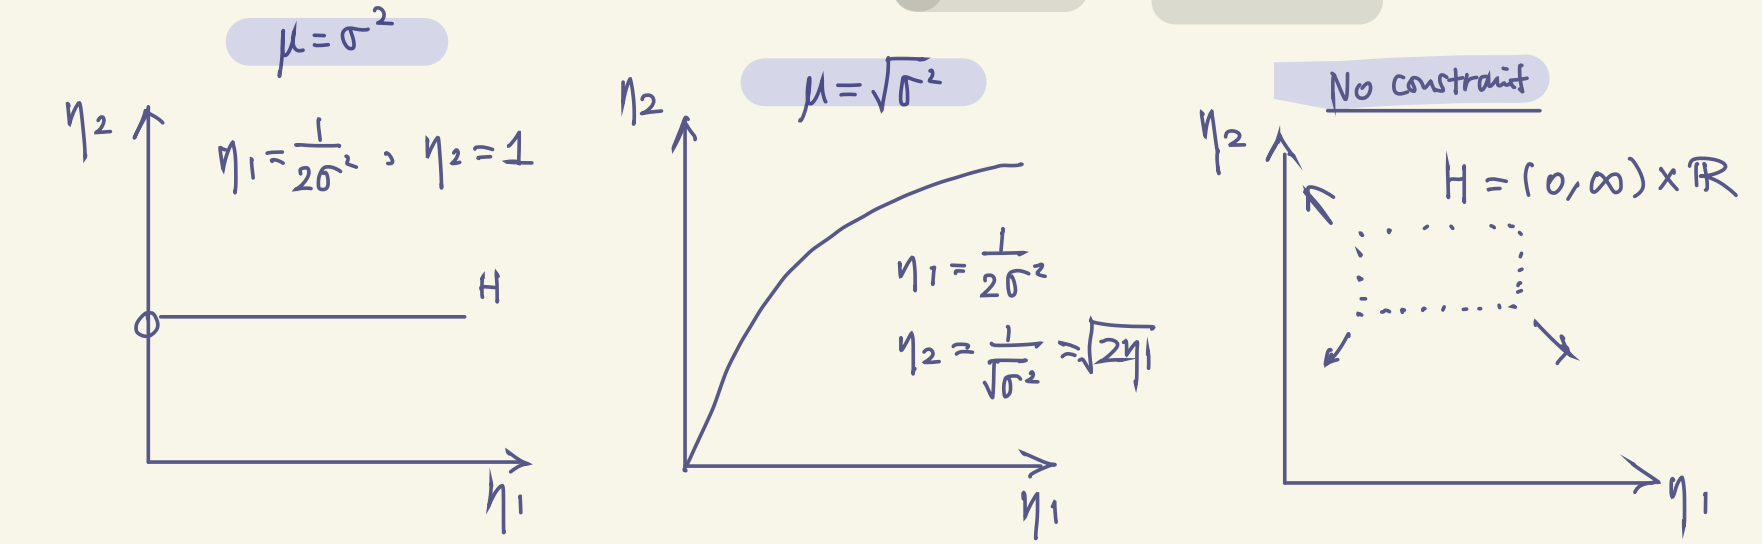
\includegraphics[width=\textwidth]{figures/fullrank-curved.png}
    \caption{curved exponential family}
    \label{fig:fullrank_curved}
\end{figure}

\begin{note}
    \textbf{Properties of Exponential Families}
    \begin{enumerate}[{(1)}]
        \item If $X_1,\cdots,X_n\overset{iid}{\sim}p(x;\theta)=
        \exp\{\sum_{i=1}^s\eta_i(\theta)T_i(x)-B(\theta)\}h(x)$, then,
        by NFFC, 
        \begin{gather}
            T=(\sum_{j=1}^nT_1(X_j),\cdots,\sum_{j=1}^nT_s(X_j))
        \end{gather}
        is sufficient.
        The exponential family data is highly compressible.
        \item If $f$ is integrable, and $\eta\in\Omega$, then
        \begin{gather}
            G(f,\boldsymbol{\eta})=\int{f(x)\exp\{\sum_{i=1}^s\eta_iT_i(x)\}h(x)d\mu(x)}
        \end{gather}
        is infinitely differentiable with respect to $\eta$ and the derivatives
        can be obtained by differentiating it under the integral sign.
        \item Moments of $T_i$'s. Take $f(x)\equiv 1$, then
        {\scriptsize
        \begin{align}
            G(1,\boldsymbol{\eta})
            =&\int{\exp\left\{ \sum_{i=1}^s\eta_iT_i(X) \right\}}h(x)d\mu(x)=\exp\{A(\boldsymbol{\eta})\}\\
            \frac{\partial{G(1,\boldsymbol{\eta})}}{\partial{\eta_i}}
            =& \int{T_i(x)\exp\left\{\sum_{i=1}^s\eta_iT_i(x)\right\}}h(x)d\mu(x)
            =\frac{\partial{A(\boldsymbol{\eta})}}{\partial{\eta_i}}=\exp\{A(\boldsymbol{\eta})\}\\
            \frac{\partial{A(\boldsymbol{\eta})}}{\partial{\eta_i}}
            =& \int{T_i(x)\exp\left\{ \sum_{i=1}^s\eta_iT_i(x)-A(\boldsymbol{\eta}) \right\}}h(x)d\mu(x)
            =\mathbb{E}_{\boldsymbol{\eta}}T_i(X)\\
            \frac{\partial^2{A(\boldsymbol{\eta})}}{\partial{\eta_i}\partial{\eta_j}}
            =& \int{T_i(x)(T_j(x)-\frac{\partial{A(\boldsymbol{\eta})}}{\partial{\eta_j}})
            \exp\left\{ \sum_{l=1}^s\eta_lT_l(x)-A(\boldsymbol{\eta}) \right\}}h(x)d\mu(x)\\
            =& \mathbb{E}_{\boldsymbol{\eta}}(T_i(X)T_j(X))
            -\mathbb{E}_{\boldsymbol{\eta}}T_i(X)
            \mathbb{E}_{\boldsymbol{\eta}}T_j(X)\\
            =& \mathrm{Cov}_{\boldsymbol{\eta}}(T_i(X),T_j(X))
        \end{align}}
    \end{enumerate}
\end{note}

\subsection{Minimal sufficiency}
\begin{definition}[Minimal sufficiency]
    A sufficient statistic $T$ is minimal 
    if for every sufficient statistic $T'$ and 
    for every $x,y\in\mathcal{X}$, 
    $T(x)=T(y)$ when $T'(x)=T'(y)$.
    In other words, $T$ is a function of $T'$,
    i.e. there exists a function $f$ such that $T(x)=f(T'(x))$ for any $x\in\mathcal{X}$.
\end{definition}

\begin{theorem}
    Let $\{p(x;\theta):\theta\in\Omega\}$ be a family of densities with respect to some measure $\mu$
    (Lebesgue measure for continuous distribution $dx$; 
    counting measure for discrete distribution $(x_i-x_{i-1})$). 
    Suppose that there exists a statistic $T$ such that, 
    for every $x,y\in\mathcal{X}$,
    \begin{gather}
        p(x;\theta)=c_{x,y}p(y;\theta)\Rightarrow T(x)=T(y)
    \end{gather}
    for every $\theta\in\Omega$ and some $c_{x,y}\in\mathbb{R}$. 
    Then $T$ is a minimal sufficient statistic.
\end{theorem}
\begin{proof}
    We first prove that $T$ is sufficient and then $T$ is minimal.

    ``$\Rightarrow$'' sufficiency for $T$:

    Start with $T(\mathcal{X})=\{t:t=T(x)~\text{for some}~x\in\mathcal{X}\}=$ range of $T$.
    For each $t\in T(\mathcal{X})$, we consider the preimage $A_t=\{x:T(x)=t\}$.
    Then, for any $y\in\mathcal{X}$, we have $y\in A_{T(y)}$ and $x_{T(y)}\in A_{T(y)}$.
    By the definition of $A_t$, we can see that $T(y)=T(x_{T(y)})$.
    Because of the assumption/condistion imposed in the statement,
    \begin{gather}
        p(y;\theta)=c_{y,x_{T(y)}}p(x_{T(y);\theta})\triangleq h(y)g_\theta(T(y))
    \end{gather}
    which implies that $T$ is sufficient as a result of the NFFC.

    ``$\Leftarrow$'' minimality of $T$:

    Consider another sufficient statistic, say $T'$. 
    By NFFC,
    \begin{gather}
        p(x;\theta)=\Tilde{g}_\theta(T'(x))\Tilde{h}(x)
    \end{gather}
    Take any $x$ and $y$ such that $T'(x)=T'(y)$, then
    \begin{align}
        p(x;\theta)
        =& \Tilde{g}_\theta(T'(x))\Tilde{h}(x)\\
        =& \Tilde{g}_\theta(T'(y))\Tilde{h}(y)\cdot\frac{\Tilde{h}(x)}{\Tilde{h}(y)}\\
        \triangleq& p(y;\theta)c_{x,y}
    \end{align}
    
    Hence, $T(x)=T(y)$ by the assumption of the minimal sufficient statistic theorem.
    So $T'(x)=T'(y)$ implies $T(x)=T(y)$ for any sufficient statistic $T'$ and any $x$ and $y$.
    Hence, $T$ is a minimal sufficient statistic.
\end{proof}

\begin{example}

    Let $X_1,\cdots,X_n\overset{iid}{\sim}\mathcal{N}(\mu,\sigma^2)$ with both $\mu$ and $\sigma^2$ unknown.
    Let $\boldsymbol{x}$ and $\boldsymbol{y}$ be any two sample points, 
    and let $(\Bar{x}_n,s_x^2)$ and $(\Bar{y}_n,s_y^2)$
    be the sample means and variances corresponding to 
    the $\boldsymbol{x}$ and $\boldsymbol{y}$ samples, respectively.

    {\footnotesize
    \begin{gather}
        \frac{p(\boldsymbol{x};\mu,\sigma^2)}{p(\boldsymbol{y};\mu,\sigma^2)}
        = \exp\left\{
        -\frac{1}{2\sigma^2}\left[
        -n(\Bar{x}_n^2-\Bar{y}_n^2)
        +2n\mu(\Bar{x}_n-\Bar{y}_n)
        -(n-1)(s_x^2-s_y^2)
        \right]
        \right\}
    \end{gather}}
    
    The ratio will be constant as a function of $\boldsymbol{\theta}=(\mu,\sigma^2)$
    if and only if $\Bar{x}_n=\Bar{y}_n$ and $s_x^2=s_y^2$. 
    Thus, by the ``theorem'', $(\Bar{x}_x,s_x^2)$ is a minimal sufficient statistic for $\boldsymbol{\theta}$,
    where $s_x^2=\frac{1}{n-1}\sum_{i=1}^n(x_i-\Bar{x}_n)^2$
\end{example}

\begin{example}
    \textbf{Curved exponential family}

    Let $X_1,\cdots,X_n\overset{iid}{\sim}\mathcal{N}(\sigma,\sigma^2)$, where $\sigma>0$, then $\theta=\sigma$
    \begin{gather}
        \frac{p(\boldsymbol{x};\mu,\sigma^2)}{p(\boldsymbol{y};\mu,\sigma^2)}
        = \exp\left\{
        -\frac{1}{2\sigma^2}\left(\sum_{i=1}^n{x_i^2}-\sum_{i=1}^n{y_i^2}\right)
        +\frac{1}{\sigma}\left(\sum_{i=1}^n{x_i}-\sum_{i=1}^n{y_i}\right)
        \right\}
    \end{gather}
    
    This ratio will be constant as a function of $\theta=\sigma$
    if and only if 
    $\sum_{i=1}^n{x_i}=\sum_{i=1}^n{y_i}$ and 
    $\sum_{i=1}^n{x_i^2}=\sum_{i=1}^n{y_i^2}$.
    Thus, by the above theorem, 
    \begin{gather}
        T(\boldsymbol{X})=(\sum_{i=1}^n X_i, \sum_{i=1}^n X_i^2)
    \end{gather}
    is minimal sufficient.
\end{example}

\begin{note}
    If $p(x;\theta)=c_{x,y}p(y;\theta)$ and $x$ and $y$ must be supported by the same $\theta$.
    (Support of $X: \{x\in\mathcal{X}:p(x;\theta)>0\}$).
    Otherwise, the ``constant'' $c_{x,y}$ will be $\theta$-dependent.
\end{note}

\begin{example}
    Let $X_1,\cdots,X_n\overset{iid}{\sim}\text{Uniform}(0,\theta)$ 
    and $T(\boldsymbol{X})=\max_{1\leq i\leq n} X_i \triangleq X_{(n)}$.
    In that case, for $\boldsymbol{x}=(x_1,\cdots,x_n)$ such that $x_i>0$,
    for $i=1,\cdots,n$,
    \begin{gather}
        p(\boldsymbol{x};\theta)
        =\prod_{i=1}^n \frac{1}{\theta}\mathbb{I}(x_i\leq \theta)
        =\frac{1}{\theta^n}\mathbb{I}\left(
        x_{(n)} < \theta
        \right)
    \end{gather}

    If $T(\boldsymbol{x})=T(\boldsymbol{y})$,
    then $p(\boldsymbol{x};\theta)=1\times p(\boldsymbol{y};\theta)$.
    The ratio between the two distributions does not depend on $\theta$,
    so $T$ is sufficient.
    
    Conversely, if $\boldsymbol{x},\boldsymbol{y}>\boldsymbol{0}$ 
    (i.e. $x_i,y_i>0$ for $i=1,\cdots,n$) are supported by the same $\theta$, then
    \begin{gather}
        \{\theta~\text{supporting}~\boldsymbol{x}\}=(T(\boldsymbol{x}),\infty)
        =(T(\boldsymbol{y}),\infty)=\{\theta~\text{supporting}~\boldsymbol{y}\}
    \end{gather}
    Therefore, $T(\boldsymbol{x})=T(\boldsymbol{y})$ and $T$ is a minimal sufficient statistic.
\end{example}

\subsection{Ancillarity \& Completeness}

\begin{example}
    Consider $X_1,\cdots,X_n\overset{iid}{\sim}\text{CauchyLoc}(\theta)$,
    whose distribution is given by 
    \begin{gather}
        p(x;\theta)=\frac{1}{\pi}\cdot\frac{1}{1+(x-\theta)^2}=f(x-\theta)
    \end{gather}
    We can see that $(X_{(1)},\cdots,X_{(n)})$ is minimal sufficient
    \footnote{refer to TPE 1.5}. 
    This is also true for the double exponential location model
    \footnote{jump diffusion;
    refer to Kou, 2002, MS}
    : $p(x,\theta)\propto\exp{(|x-\theta|)}$
\end{example}

\begin{question}
    What determines the level of compressibility?
\end{question}

\begin{definition}[Ancillarity]
    A statistic $A$ is ancillary for $X\sim p_\theta \in \mathcal{P}$
    if the distribution of $A(\boldsymbol{X})$ does not depend on $\theta$.
\end{definition}

\begin{example}
    Consider again $X_1,\cdots,X_n\overset{iid}{\sim}\text{CauchyLoc}(\theta)$,
    and define $A(\boldsymbol{X})=X_{(n)}-X_{(1)}$,
    which can be rewritten as $A(\boldsymbol{X})=(Z_{(n)}+\theta)-(Z_{(1)}+\theta)$,
    and we can see that $A(\boldsymbol{X})$ is ancillary w.r.t. $\theta$
\end{example}

\begin{solution} 
    Answer for Question 1.\\
    The statistic that we make use of should include as little ancillary information as possible.
\end{solution}

\begin{definition}[first-order ancillary statistic]
    A statistics $A$ is first-order ancillary for $X\sim p_\theta\in\mathcal{P}$
    if $\mathbb{E}_\theta A(\boldsymbol{X})$ does not depend on $\theta$.
\end{definition}

\begin{definition}[Completeness]
    A statistic $T$ is complete for $X\sim p_\theta\in\mathcal{P}$
    if no non-constant function of $T$ is first-order ancillary.
    In other words, if $\mathbb{E}_\theta{f(T(\boldsymbol(X)))}=0~\forall{\theta}$,
    thus $f(T(\boldsymbol{X}))=0$ with probability 1 for all $\theta$.
\end{definition}

Completeness formalizes our ideal concept of optimal data reduction.
Minimal sufficiency is our achievable notion of optimal data reduction.

\textbf{Properties}:
\begin{enumerate}
    \item If $T$ is complete sufficient, then $T$ is minimal sufficient. 
    This is known as Bahadur's theorem.
    \item Complete sufficient statistics yield optimal unbiased estimators
\end{enumerate}

\begin{example}
    Let $X_1,\cdots,X_n\overset{iid}{\sim}\text{Bernoulli}(\theta),~\theta\in(0,1)$.
    Then we know that $T(\boldsymbol{X})=\sum_{i=1}^n{X_i}$ is sufficient.
    Sippose $\mathbb{E}_\theta f(T(\boldsymbol{X}))=0$ for all $\theta\in(0,1)$. Observe
    \begin{gather}
        \mathbb{E}_\theta f(T(\boldsymbol{X}))
        =\sum_{i=1}^n{f(i)\binom{n}{i}\theta^i(1-\theta)^{n-i}}=0~\forall{\theta}\in(0,1)\label{eq:compex1}
    \end{gather}
    Dividing Equation (\ref{eq:compex1}) through by $\theta^n$ and let $\beta=\frac{\theta}{1-\theta}$, we have
    \begin{gather}
        \sum_{i=1}^n{f(i)\binom{n}{i}\beta^i}=0~\forall{\beta}>0.\label{eq:compex2}
    \end{gather}

    If $f$ are non-zero, then the LHS of Equation (\ref{eq:compex2}) is a polynomial of degree at most $n$.
    However, an n-th degree polynomial can have at most n roots. 
    Hence, it is impossible for the LHS to equal 0 for every $\beta>0$ unless $f=0$.
    We can conclude that $T$ is complete.
\end{example}

\begin{example}
    Let $X_1,\cdots,X_n\overset{iid}{\sim}\mathcal{N}(\theta,\sigma^2)$, with $\theta\in\mathbb{R}$ unknown and 
    a known $\sigma^2>0$, Is $\Bar{X}_n=\frac{1}{n}\sum_{i=1}^nX_i$ 
    (we know it minimal sufficient) complete for this model?

    To simplify the notation, we consider a special case where $n=1$ and $\sigma=1$,
    so that $T(X)=X\sim \mathcal{N}(\theta,1)$. Suppose
    \begin{gather}
        \mathbb{E}_\theta f(X)
        =\frac{1}{\sqrt{2\pi}}\int_{-\infty}^\infty{f(x)\exp\{-\frac{(x-\theta)^2}{2}\}}dx=0
        ~\forall\theta\in\mathbb{R}.\label{eq:minicompex}
    \end{gather}
    Multiplying both sides by $\sqrt{2\pi}e^\frac{\theta^2}{2}$,
    we can rewrite Equation (\ref{eq:minicompex}) as 
    \begin{gather}
        \int_{\infty}^\infty{f(x)\exp\{ -\frac{x^2}{2}\}\exp\{\theta x\}}dx=0
        ~\forall{\theta}\in\mathbb{R}\label{eq:minicompex2}
    \end{gather}
    
    We decompose $f$ into its positive and negative parts as $f=f^+-f^-$, 
    where $f^+(x)=\max(f(x),0)$ and $f^-(x)=\max(-f(x),0)$.
    Observe that $f^+(x)\geq 0$ and $f^-(x)\geq 0$ for all $x\in\mathbb{R}$ and
    $f^+(x)=f^-(x)$ if and only if $f^+(x)=f^-(x)=0$.
    If $f(x)\geq 0$ a.e. or $f(x)\leq 0$ a.e., 
    then Equation (\ref{eq:minicompex2}) implies that $f(x)=0$ a.e. because
    setting $\theta=0$ gives us an integral of a non-negative (or a non-positive) function.

    We may write
    \begin{gather}
        \frac{\int_{-\infty}^\infty{\color{red}f^+(x)\exp\{-\frac{x^2}{2}\}}\exp\{\theta x\}dx}
        {\color{red}\int_{-\infty}^\infty f^+(x)\exp\{-\frac{x^2}{2}\}dx}
        =
        \frac{\int_{-\infty}^\infty{\color{blue}f^-(x)\exp\{-\frac{x^2}{2}\}}\exp\{\theta x\}dx}
        {\color{blue}\int_{-\infty}^\infty f^-(x)\exp\{-\frac{x^2}{2}\}dx}
        \label{eq:minicompex3}
    \end{gather}
    Notice that in Equation (\ref{eq:minicompex3}), 
    the part of {\color{red} red} or {\color{blue} blue} defines a legitimate probability density and 
    notice that both sides of Equation (\ref{eq:minicompex3}) is the MGF of this density. We have 
    \begin{gather}
        M_{f^+}(t)=M_{f^-}(t)
    \end{gather}
    which implies that $f^+(x)=f^-(x)$ a.e. or, in other words, 
    $f^+=f^-=0$ a.e., i.e. $f(X)=0$ a.s.. 
    Hence $T$ is sufficient and complete.
\end{example}

\begin{exercise}
    If $X\sim p(x;\theta)\propto h(x)\exp\{\theta x\}$, then the statistic $T(X)=X$ is complete.

    \textbf{Keysteps:}
    \begin{enumerate}[{(1)}]
        \item Suppose $\int{f(x)h(x)\exp\{\theta x\}}dx=0~\forall{\theta}$;
        \item Decompose $f=f^+-f^-$ with $f^+,f^-\geq 0$;
        \item $f^+$ and $f^-$ can be viewed as legitimate density;
        \item The decomposition shows that the MGF's of $f^+$ and $f^-$ coincide and hence $f\equiv{0}$.
    \end{enumerate}
\end{exercise}

\begin{theorem}
    $(T_1,\cdots,T_s)$ is complete for any s-dimensional full rank exponential family\footnote{TSH}.
\end{theorem}

\begin{theorem}
    \textbf{Basu's Theorem}\\
    If $T$ is complete and sufficient for $\mathcal{P}=\{p_\theta:\theta\in\Omega\}$
    and $V$ is ancillary, then $T(\boldsymbol{X})$ \rotatebox{90}{$\models$} $V(\boldsymbol{X})$.
\end{theorem}
\begin{proof}
    Define $q_A(t)=P_\theta(V\in A|T=t)$ and $p_A=P_\theta(V\in A)$.
    By sufficiency and ancillarity, neither $p_A$ nor $q_A(t)$ depends on $\theta$.
    By smoothing/tower expectation, 
    we can write
    \begin{gather}
        p_A=P_\theta(V\in A)=\mathbb{E}_\theta P_\theta(V\in A|T)=\mathbb{E}_\theta q_A(T)
    \end{gather}
    By completeness,
    \begin{gather}
        \mathbb{E}_\theta(q_A(T)-p_A)\triangleq\mathbb{E}_\theta{f(T)}=0
    \end{gather}
    Hence, 
    \begin{gather}
        f(T)=q_A(T)-p_A=0~\text{i.e.}~q_A(T)=p_A
    \end{gather}
    Again by smoothing/tower expectation,
    \begin{align}
        P_\theta(T\in B,V\in A)
        =& \mathbb{E}_\theta[\mathbf{1}_B(T)\mathbf{1}_A(V)]~~{\color{gray} \mathbf{1}_B(T)=\mathbb{I}(T\in B)}\\
        =& \mathbb{E}_\theta\{\mathbb{E}_\theta[\mathbf{1}_B(T)\mathbf{1}_A(V)|T]\}\\
        =& \mathbb{E}_\theta\{\mathbf{1}_B(T)\mathbb{E}_\theta[\mathbf{1}_A(V)|T]\}\\
        =& \mathbb{E}_\theta[\mathbf{1}_B(T)q_A(T)]\\
        =& \mathbb{E}_\theta[\mathbf{1}_B(T)p_A]\\
        =& p_A\mathbb{E}_\theta\mathbf{1}_B(T)\\
        =& P_\theta(V\in A)P_\theta(T\in B)
    \end{align}
    Hence, $T$ and $V$ are independent as $A$ and $B$ are arbitrary Beorel sets.
\end{proof}

\begin{example}
    Let $X_1,\cdots,X_n\overset{iid}{\sim}\mathcal{N}(\mu,\sigma^2)$, 
    where both $\mu$ and $\sigma^2$ are unknown. 
    Then $\Bar{X}_n$ \rotatebox{90}{$\models$} $\frac{1}{n}\sum_{i=1}^n(X_i-\Bar{X}_n)^2$.
    
    For any $\sigma>0$, we consider the submodel $\mathcal{P}_\sigma\{\mathcal{N}(\mu,\sigma^2):\mu\in\mathbb{R}\}$.
    In each submodel, $\Bar{X}_n$ is complete and sufficient, 
    and $\frac{1}{n}\sum_{i=1}^n(X_i-\Bar{X}_n)^2$ is ancillary. 
    (Let $X_i=Z_i+\mu$, then $X_i-\Bar{X}_n=Z_i-\Bar{Z}_n$, 
    which does not depend on $\mu$.)

    By Basu's theorem, $\Bar{X}_n$ \rotatebox{90}{$\models$} $\sum_{i=1}^n(X_i-\Bar{X}_n)^2$
    under $\mathcal{N}(\mu,\sigma^2)$ for any $\mu$.
    Since $\sigma$ is arbitrary, we can conclude that 
    $\Bar{X}_n$ \rotatebox{90}{$\models$} $\frac{1}{n}\sum_{i=1}^n(X_i-\Bar{X}_n)^2$
    holds for the full model $\mathcal{P}=\{\mathcal{N}(\mu,\sigma^2):\mu\in\mathbb{R},\sigma^2>0\}$.
\end{example}

\subsection{From Data Reduction to Optimal Inference}
\begin{enumerate}
    \item Lossless data reduction (Sufficiency)
    \item Optimal data reduction (Minimal sufficiency + completeness)
    \item \textbf{Optimal inference/estimation}
\end{enumerate}

\begin{definition}[Convex function]
    A function $f$ is a convex function if $x\neq y$ and $\gamma\in(0,1)$
    \begin{gather}
        f(\gamma x+(1-\gamma) y) \leq \gamma f(x) + (1-\gamma) f(y)
    \end{gather}

    The function $f$ is said to be strictly convex if the above inequality holds strictly (i.e. ``$<$'').
\end{definition}


\begin{example}
    As Shown in Figure \ref{fig:convex}
    \begin{enumerate}
        \item For any $\theta\in\Omega$, the function $f(d)=(d-\theta)^2$ is strictly convex on $\mathbb{R}$.
        \item For any $\theta\in\Omega$, the function $f(d)=|d-\theta|$ is convex but not strictly convex.
    \end{enumerate}
\end{example}

\begin{figure}[htpb]
    \centering
    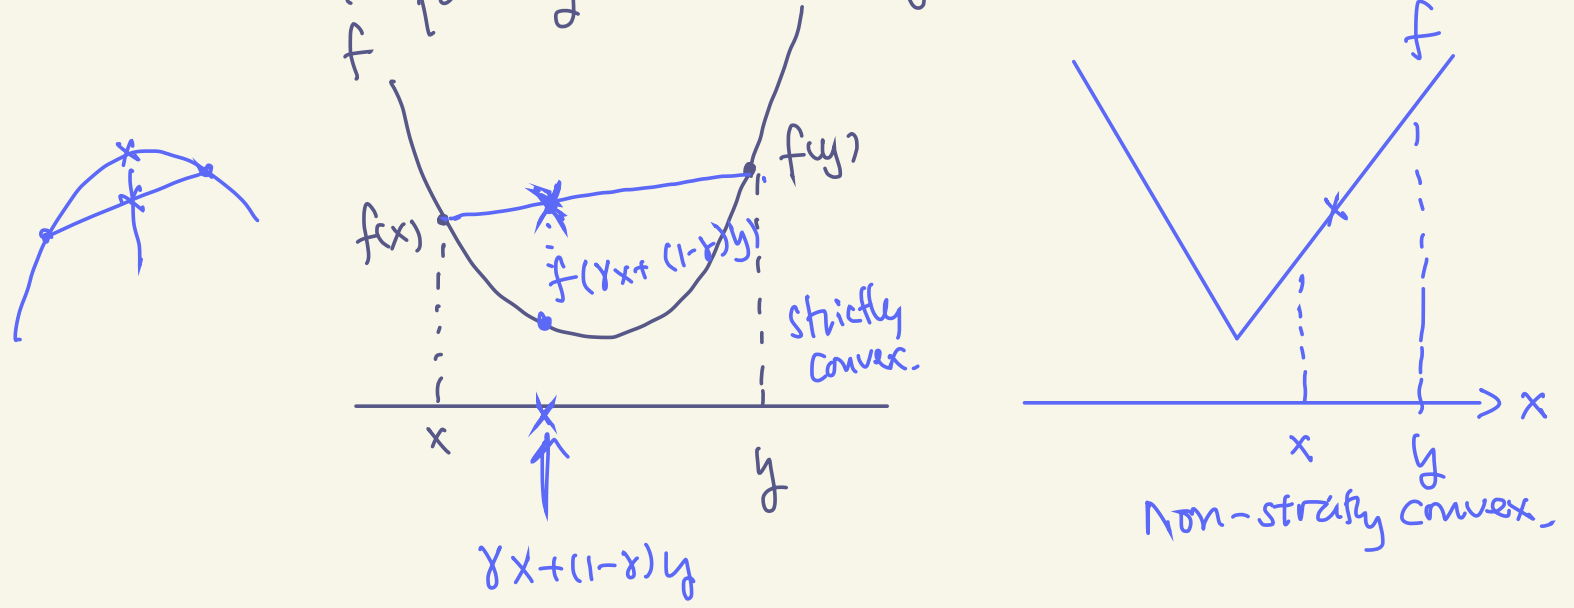
\includegraphics[width=\textwidth]{figures/convex.png}
    \caption{Convex functions}
    \label{fig:convex}
\end{figure}

\begin{theorem}
    \textbf{Jensen's Inequality}\\
    For a convex $f$, and $\mathbb{E}X$ exists, then
    \begin{gather}
        f(\mathbb{E}X)\leq\mathbb{E}f(X)
    \end{gather}
    If $f$ is strictly convex, then the above inequality holds strictly unless 
    $X=\mathbb{E}X$ with probability 1.
\end{theorem}


\begin{theorem}\label{thm:raoblackwell}
    \textbf{Rao-Blackwell Theorem}\\
    Suppose $T$ is sufficient for $\mathcal{P}=\{p_\theta: \theta\in\Omega\}$,
    that $\delta(\boldsymbol{X})$ is an estimator for $g(\theta)$ for which $\mathbb{E}\delta(\boldsymbol{X})$ exists,
    and that $R(\theta,\delta)=\mathbb{E}_\theta L(\theta,\delta(\boldsymbol{X}))<\infty$.
    If, in particular, $L(\theta,\cdot)$ is convex, then
    \begin{gather}
        R(\theta, \eta)\leq R(\theta,\delta)\\
        \text{for}~\eta=\mathbb{E}[\delta(\boldsymbol{X})|T(\boldsymbol{X})]
    \end{gather}
    If $L(\theta,\cdot)$ is strictly convex, then $R(\theta,\eta)<R(\theta,\delta)$
    for any $\theta$ unless $\eta(T(\boldsymbol{X}))=\delta(\boldsymbol{X})$ with probability 1.
\end{theorem}


\begin{example}
    If $X_1,\cdots,X_n\overset{iid}{\sim}\text{Bernoulli}(\theta)$, where $\theta\in(0,1)$.
    Consider $L(\theta,d)=(\theta-d)^2$. 
    Suppose we have a naive estimator $\delta(\boldsymbol{X})=X_1$.
    We know that $T(X)=\Bar{X}_n$ is sufficient,
    so we can apply the Rao-Blackwell Theorem to \textbf{improve an estimator $\delta$}:
    \begin{align}
        \eta(T(\boldsymbol{X}))
        =& \mathbb{E}[\delta(\boldsymbol{X})|T(\boldsymbol{X})]\\
        =& \frac{1}{n}\sum_{i=1}^n\mathbb{E}[\delta(\boldsymbol{X})|\Bar{X}_n]\\
        =& \mathbb{E}(\Bar{X}_n|\Bar{X}_n) = \Bar{X}_n
    \end{align}
    Recall that 
    \begin{gather}
        R(\theta,\eta)=\frac{\theta(1-\theta)}{n}<\theta(1-\theta)=R(\theta,\delta)
    \end{gather}
\end{example}

\newpage
  \lesson{original Lecture 6 -- 10}{Point Estimation}

\subsection{UMVUE}

\begin{definition}[unbiased estimator]
    An estimator is said to be unbiased 
    if $\mathbb{E}_\theta\delta(\boldsymbol{X})=g(\theta)$ for all $\theta$.
\end{definition}

Finding the uniformly best estimator is challenging,
but we can  find an unbiased estimator that gives minimum risk uniformly,
i.e. $R(\theta,\delta)\leq R(\theta,\delta')$ for all $\theta\in\Omega$
and any other unbiased estimator.
Such an estimator is called a \textbf{uniformly minimum risk unbiased estimator} (UMRUE).
In particular, if we adapt $L(\theta, d)=(\theta-d)^2$,
an UMRUE will become a \textbf{uniformly minimum variance unbiased estimator} (UMVUE), because
\begin{gather}
    \underbrace{\mathbb{E}_\theta[g(\theta)-\delta(\boldsymbol{X})]^2}_{\text{MSE}}
    =\underbrace{[\mathbb{E}_\theta\delta(\boldsymbol{X})-g(\theta)]^2}_{\text{Bias}^2}
    +\underbrace{\mathbb{E}_\theta[\delta(\boldsymbol{X})-\mathbb{E}_\theta\delta(\boldsymbol{X})]^2}_{\text{variance of}~\delta(\boldsymbol{X})}
\end{gather}
and if $\delta(\boldsymbol{X})$ is unbiased,
then the MSE will reduced to 
\begin{gather}
    \mathbb{E}_\theta[g(\theta)-\delta(\boldsymbol{X})]^2
    =\mathbb{E}_\theta[\delta(\boldsymbol{X})-\mathbb{E}_\theta\delta(\boldsymbol{X})]^2
\end{gather}

\begin{definition}[U-estimatable]
    If an unbiased estimator exists, then $g(\cdot)$ is called U-estimatable.
\end{definition}

\begin{example}
    Suppose $X\sim\text{Unifrom}(0,\theta)$, then $\delta({X})$ if 
    \begin{gather}
        \int_0^\theta\frac{\delta({x})}{\theta}d{x}=g(\theta)~\forall{\theta}>0
    \end{gather}
    or if 
    \begin{gather}
        \int_0^\theta \delta({x})d{x}=g(\theta)~\forall{\theta}>0 \label{eq:umvueex1}
    \end{gather}
    So, $g$ cannot be U-estimatable unless $\theta g(\theta)\to 0$ as $\theta\downarrow 0$.
    If $g'$ exists, hen differentiating Equation (\ref{eq:umvueex1}),
    and also by the fundamental theorem of calculus, we have
    \begin{gather}
        \delta(\boldsymbol{x})=\frac{\partial}{\partial{x}}[xg(x)]=g(x)+xg'(x)
    \end{gather}
    For example, say $g(\theta)=\theta$, then $\delta(X)=X+X\cdot 1=2X$.
\end{example}

\begin{example}
    Suppose $X\sim\text{Binomial}(n\theta)$. 
    If $g(\theta)=\sin\theta$, then $\delta(X)$ will be unbiased if 
    \begin{gather}
        \sum_{k=0}^n\delta(k)\binom{n}{k}\theta^k(1-\theta)^{n-k}=\sin\theta~\forall{\theta}\in(0,1).\label{eq:umvueex2}
    \end{gather}
    The LHS of Equation (\ref{eq:umvueex2}) is a polynomial in $\theta$ with degree at most $n$.
    The sine function cannot be written as a polynomial of degree $n$.
    Therefore, $\sin\theta$is not U-estimatable.
\end{example}

\begin{definition}[UMVU]
    An unbiased estimator $\delta$ is uniformly minimum variance unbiased (UMVU) if 
    \begin{gather}
        \mathrm{Var}_\theta \delta\leq \mathrm{Var}_\theta\delta'~\forall\theta\in\Omega
    \end{gather}
    and for any other competing unbiased estimator $\delta'$.
\end{definition}

\begin{theorem}
    \textbf{Lehmann-Scheff$\bm{\acute{e}}$ Theorem}\\
    If $T$ is a complete and sufficient statistic, and $\mathbb{E}_\theta h(T(\boldsymbol{X}))=g(\theta)$,
    i.e. $h(T(\boldsymbol{X}))$ is unbiased for $g(\theta)$,
    then $h(T(\boldsymbol{X}))$ is
    \begin{enumerate}[{(a)}]
        \item the only functon of $T(\boldsymbol{X})$ that is unbiased for $g(\theta)$;
        \item an UMRUE under any convex loss function;
        \item the unique UMVRE (hence UMVUE), up to a P-null set, 
        under any strictly convex loss function.
    \end{enumerate}
\end{theorem}
\begin{proof}
    $~$
    \begin{enumerate}[{(a)}]
        \item Suppose $\mathbb{E}_\theta\Tilde{h}(T(\boldsymbol{X}))=g(\theta)$, then
        \begin{gather}
            \mathbb{E}_\theta[\Tilde{h}(T(\boldsymbol{X}))-h(T(\boldsymbol{X}))]=0~\forall{\theta}\in\Omega.
        \end{gather}
        Thus, $\Tilde{h}(T(\boldsymbol{X}))=h(T(\boldsymbol{X}))$ a.s. 
        for all $\theta\in\Omega$ by completeness.
        \item Consider any unbiased estimator $\delta(\boldsymbol{X})$ and 
        let $\Tilde{h}(T(\boldsymbol{X}))=\mathbb{E}_\theta[\delta(\boldsymbol{X})|T(\boldsymbol{X})]$. Then
        \begin{gather}
            \mathbb{E}_\theta\Tilde{h}(T(\boldsymbol{X}))
            =\mathbb{E}_\theta\{\mathbb{E}_\theta[\delta(\boldsymbol{X})|T(\boldsymbol{X})]\}
            =\mathbb{E}_\theta\delta(\boldsymbol{X})=g(\theta)
        \end{gather}
        by smoothing. By (a), $\Tilde{h}(T(\boldsymbol{X}))=h(T(\boldsymbol{X}))$, then
        \begin{gather}
            R(\theta,\Tilde{h}(T(\boldsymbol{X})))=R(\theta,h(T(\boldsymbol{X}))).
        \end{gather}
        By Rao-Blackwell Theorem, we have 
        \begin{gather}
            R(\theta,h(T(\boldsymbol{X})))\leq R(\theta,\delta)~\forall{\theta}\in\Omega.
        \end{gather}
        Therefore, $h(T(\boldsymbol{X}))$ is an UMRUE for any convex loss function.
        \item If the loss function is strictly convex, 
        $R(\theta,h(T(\boldsymbol{X})))< R(\theta,\delta)$
        unless $\delta(\boldsymbol{X})\overset{a.s.}{=}h(T(\boldsymbol{X}))$. 
        Hence, $h(T(\boldsymbol{X}))$ is the unique UMRUE
        (UMVUE if the loss function is the squared error loss function).
    \end{enumerate}
\end{proof}

\begin{note}
    \textbf{How can we find a UMVUE?} The possible solutions include
    \begin{enumerate}[{(a)}]
        \item Rao-Blackwellization
        \item Solve for $\delta$ directly
        \item Guess
    \end{enumerate}
\end{note}


\begin{example}
    \textbf{Rao-Blackwellisation}\\
    Suppose $X_1,\cdots,X_n\overset{iid}{\sim}\text{Bernoulli}(\theta)$.
    We know that $T(\boldsymbol{X})=\sum_{i=1}^nX_i$ is a complete sufficient statistic,
    we also know that $n^{-1}T(\boldsymbol{X})$ is an unbiased estimator for $\theta$,
    i.e.$\mathbb{E}_\theta\frac{T(\boldsymbol{X})}{n}=\theta$.
    Therefore, $n^{-1}T()\boldsymbol{X}$ is an UMRUE for $\theta$ under any convex loss function.

    Suppose that, instead, we are interested in estimating $\theta^2$. 
    Let's observe 
    \begin{align}
        \delta(\boldsymbol{X})=&\mathbb{I}(X_1=X_2=1)=X_1X_2\\
        \mathbb{E}_\theta\delta(\boldsymbol{X})=&\mathbb{E}_\theta(X_1X_2)=(\mathbb{E}_\theta X_1)^2=\theta^2\\
        \mathbb{E}_\theta[\delta(\boldsymbol{X})|T(\boldsymbol{X})=t]
        =& P_\theta(X_1=X_2=1|T(\boldsymbol{X})=t)\\
        =& \frac{P_\theta(X_1=X_2=1, \sum_{i=3}^n = t-2)}{P_\theta(T(\boldsymbol{X})=t)}\\
        =& \frac{\theta^2\binom{n-2}{t-2}\theta^{t-2}(1-\theta)^{n-t}\mathbb{I}(t\geq 2)}{\binom{n}{t}\theta^t(1-\theta)^{n-t}}\\
        =& \frac{t(t-1)\mathbb{I}(t\geq 2)}{n(n-1)}
    \end{align}
    Hence, we conclude that a UMRUE for $\theta^2$ is $\frac{T(\boldsymbol{X})(T(\boldsymbol{X})-1)}{n(n-1)}$.
\end{example}

\begin{example}
    Suppose $X_1,\cdots,X_n\overset{iid}{\sim}\text{U}(0,\theta)$.
    In this case $T(\boldsymbol{X})=X_{(n)}$ is a complete and sufficient statistic,
    and $\delta(X)=2X$ is a unbiased estimator for $\theta$, 
    i.e. $\mathbb{E}_\theta(2X)=2\cdot\frac{\theta}{2}=\theta$.

    Given $X_{(n)}$, $X_1$ is equal to $X_{(n)}$ with probability $\frac{1}{n}$
    and follows $\text{U}(0,X_{(n)})$ with probability $1-\frac{1}{n}$.
    Hence,
    \begin{gather}
        P_\theta(X_1=x_1|T(\boldsymbol{X}))
        =\frac{\mathbb{I}(T(\boldsymbol{X})=x_1)}{n}
        +\underbrace{\frac{\mathbb{I}(0<x_1<T(\boldsymbol{X}))}{T(\boldsymbol{X})}}_{\text{uniform}}(1-\frac{1}{n})
    \end{gather}

    To find the UMVUE, we calculate 
    \begin{align}
        \mathbb{E}_\theta(\delta(X)|T(\boldsymbol{(X}))
        =& 2\mathbb{E}_\theta(X_1|T(\boldsymbol{X}))\\
        =& 2\left[ \frac{1}{n}T(\boldsymbol{X}) + (1-\frac{1}{n})\int_{0}^{T(\boldsymbol{X})}\frac{x_1}{T(\boldsymbol{X})}dx_1 \right]\\
        =& 2\left[ \frac{T(\boldsymbol{X})}{n} + (1-\frac{1}{n})\frac{T(\boldsymbol{X})}{2} \right]\\
        =& \frac{n+1}{n}T(\boldsymbol{X})
    \end{align}
    which gives the desired result.
\end{example}

\begin{example}
    \textbf{Solve for $\delta$ directly}\\
    Let $X\sim\text{Poisson}(\theta)$. 
    $X$ is a complete and sufficient statistic for $theta$.
    $X$ is also unbiased and therefore UMVU for $\theta$.
    Suppose we are interested in estimating $g(\theta)=e^{-a\theta}$ for $a\in\mathbb{R}$.
    We need to find an estimator $\delta$ such that $\mathbb{E}_\theta\delta(X)=g(\theta)$ for all $\theta>0$.
    Under this model, we have
    \begin{align}
        &\mathbb{E}_\theta\delta(X)=\sum_{x=0}^\infty\delta(x)\frac{e^{-\theta}\theta^x}{x!}=e^{-a\theta},~\forall{\theta}>0\\
        \Leftrightarrow& \sum_{x=0}^\infty\frac{\delta{x}\theta^x}{x!}=e^{(1-a)\theta}=\sum_{x=0}^\infty\frac{(1-a)^x\theta^x}{x!}\\
        \Rightarrow& \delta(X)=(1-a)^X
    \end{align}
    is the UMVUE for $g(\theta)$.

    Note that this estimator B not ideal in the sense that if $a = 2$,
    then the estimator $\delta(X) = (-1)^X$ will change sign according to
    the ``evenness'' of $X$. 
    The estimator is hence inadmissible when $a > 1$ and will be
    dominated by $\max(\delta(X),0)$.
\end{example}

\begin{example}
    \textbf{Guess}\\
    Let $X_1,\cdots,X_n\overset{iid}{\sim}\mathcal{N}(\mu,\sigma^2)$. 
    Consider the case when $\boldsymbol{\theta}=(\mu,\sigma^2)$ is unknown.
    Show that
    \begin{enumerate}[{(i)}]
        \item The UMVUE for $\sigma^2=(n-1)^{-1}\sum_{i=1}^n(X_i-\Bar{X}_n)^2=\delta^2$.
        \item How about the UMVUE for $\sigma$?
        \item What is the UMVUE for $\mu^2$?
    \end{enumerate}

    \textbf{Solution}:
    \begin{enumerate}[{(i)}]
        \item {\color{red}[WAIT TO BE DONE...]}
        \item Observe $X_i-\Bar{X}_n\sim \mathcal{N}(0,\frac{n-1}{n}\sigma^2)$ and 
        $\mathbb{E}|X_i-\Bar{X}_n|=\sigma\sqrt{\frac{2}{\pi}}\cdot\sqrt{\frac{n-1}{n}}$.
        This implies that 
        \begin{gather}
            \delta'=\left.\sqrt{\frac{\pi n}{2(n-1)}}|X_i-\Bar{X}_n|\right|S
        \end{gather}
        is unbiased for $\sigma$. Instead, we can observe another fact that 
        \begin{gather}
            S_*^2=\sum_{i=1}^n(X_i-\Bar{X}_n)^2=(n-1)S^2 \sim \sigma^2\chi^2_{n-1}
        \end{gather}
        Hence,
        \begin{gather}
            \mathbb{E}S_*=\sigma\mathbb{E}\chi_{n-1}\Rightarrow\sigma=\frac{\mathbb{E}S_*}{\mathbb{E}\chi_{n-1}},
        \end{gather}
        meaning that $\frac{S_*}{\mathbb{E}\chi_{n-1}}$ is unbiased for $\sigma$ and hence UMVUE.
        \item Take the expectation of the UMVUE for $\mu$ and square it,
        we obtain $\mathbb{E}\Bar{X}_n^2=\mu^2+\frac{\sigma^2}{n}$ and so, 
        \begin{gather}
            \delta_n(X)=\underbrace{\Bar{X}_n^2-\frac{S_*^2}{n(n-1)}}_{\text{may be negative}}
        \end{gather}
        is UMVUE for $\mu^2$.
    \end{enumerate}
\end{example}

\subsection{Fisher Information}

Let $X_1,\cdots,X_n\overset{iid}{\sim}\mathcal{N}(\mu,\sigma^2)$. 
Define $s^2=\sum_{i=1}^n(X_i-\Bar{X}_n)^2$,
$\frac{s^2}{n-1}$ is the UMVUE for $\sigma^2$, and
$\frac{s^2}{n}$ is the MLE for $\sigma^2$, 
none of which and no other estimators, 
like shrunk estimator ($\frac{s^2}{n+1}$) and James-Stein estimator,
are admissible.

\begin{question}
    Suppose we have $\delta_1$ and $\delta_2$ as UMVUEs for $g_1(\theta)$ and $g_2(\theta)$, respectively.
    Is $\delta_1 + \delta_2$ an UMVUE for $g_1(\theta)+g_2(\theta)$?
\end{question}

\begin{theorem}
    \textbf{Characterization of UMVUEs}\footnote{TPE 2.1.7}\\
    Let $\Delta=\{\delta:\mathbb{E}_\theta\delta^2<\infty\}$. 
    Then $\delta_0\in\Delta$ is UMVUE for $g(\theta)=\mathbb{E}\delta_0$
    if and only if 
    \begin{gather}
        \mathbb{E}[\delta(X)U]~\forall{U}\in\mathcal{U}\triangleq\{U:\mathbb{E}U=0\}.
    \end{gather}
\end{theorem}
\begin{proof}
    If $\delta_0$ is an UMVUE, 
    let's consider $\delta_\lambda=\delta_0 + \lambda{U}$ for a fixed $\lambda\in\mathbb{R}$ and $U\in\mathcal{U}$.
    Since $\delta_0$ has minimal variance,
    \begin{gather}
        \mathrm{Var}_\theta\delta_\lambda
        =\mathrm{Var}_\theta\delta_0+\lambda^2\mathrm{Var}_\theta{U}+2\lambda\mathrm{Cov}_\theta(\delta_0,U)
        \geq\mathrm{Var}_\theta\delta_0,
    \end{gather}
    or equivalently,
    \begin{gather}
        \lambda^2\mathrm{Var}_\theta{U}+2\lambda\mathrm{Cov}_\theta(\delta_0,U)\geq 0.
    \end{gather}

    Consider the quadratic form 
    \begin{gather}
        q(\lambda)=\lambda^2\mathrm{Var}_\theta{U}+2\lambda\mathrm{Cov}_\theta(\delta_0,U),
    \end{gather}
    which has the roots
    \begin{gather}
        \lambda=0~\text{and}~\lambda=\frac{-2\mathrm{Cov}_\theta(\delta_0,U)}{\mathrm{Var}_\theta{U}}
    \end{gather}
    If the roots are distinct, the form must be negative at some point,
    which violates the inequality above.
    Hence $\frac{-2\mathrm{Cov}_\theta(\delta_0,U)}{\mathrm{Var}_\theta{U}}=0$
    in which case $\mathrm{E}_\theta[\delta_0 U]=\mathrm{Cov}_\theta(\delta_0,U)=0$.

    We assume that $\mathrm{E}_\theta[\delta_0 U]=0$ for all $U\in\mathcal{U}$, 
    and consider any $\delta$ unbiased for $g(\theta)$. 
    It follows that $\delta-\delta_0\in\mathcal{U}$.
    So $\mathbb{E}_\theta[\delta_0(\delta-\delta_0)]=0$.
    This implies that $\mathbb{E}_\theta(\delta_0\delta)=\mathbb{E}_\theta\delta_0^2$ and 
    subtracting $\mathbb{E}_\theta^2\delta_0(=\mathbb{E}_\theta\delta_0\mathbb{E}_\theta\delta)$ on both sides,
    we obtain
    \begin{gather}
        \mathrm{Var}_\theta\delta_0=\mathrm{Cov}_\theta(\delta_0,\delta)
        \overset{\text{Cauchy}}{\leq}\sqrt{\mathrm{Var}_\theta\delta_0\mathrm{Var}_\theta\delta}
    \end{gather}
    Hence, $\mathrm{Var}_\theta\delta_0\leq\mathrm{Var}_\theta\delta$ for any arbitrary unbiased estimator $\delta$.
    Hence $\delta_0$ is a UMVUE for $g(\theta)$.
    \begin{gather}
        \mathbb{E}_\theta[(\delta_1+\delta_2)U]=\mathbb{E}_\theta(\delta_1U)+\mathbb{E}_\theta(\delta_2U) = 0~\forall{U}\in\mathcal{U}
    \end{gather}
    $\Rightarrow \delta_1+\delta_2$ is a UMVUE of $g_1(\theta)+g_2(\theta)$.
\end{proof}

\subsubsection{Variance Bounds and Information}

Recall from the Cauchy-Schwarz Inequality,
\begin{gather}
    \mathrm{Cov}(X,Y)\leq\sqrt{\mathrm{Var}X\mathrm{Var}Y}~\text{or}~|\mathrm{Cov}(X,Y)|\leq\sigma_X\sigma_Y.
\end{gather}

If $\delta$ is an unbiased estimator for $g(\theta)$ and $\psi$ is an arbitrary suitable r.v.
so that the $\mathrm{Cov}_\theta(\delta,\psi)$ is the same for all $\delta$ that are unbiased for $g(\theta)$, then
\begin{gather}
    \mathrm{Var}_\theta\delta\geq\frac{\mathrm{Cov}_\theta^2(\delta,\psi)}{\mathrm{Var}_\theta\psi}
\end{gather}

Let $\mathcal{P}=\{p_\theta:\theta\in\Omega\}$ be a dominated family with densities $f_\theta:\theta\in\Omega=\mathbb{R}$.
To begin, $\mathbb{E}_{\theta+\Delta}\delta-\mathbb{E}_\theta\delta$ gives $g(\theta+\Delta)-g(\theta)$ for any unbiased $\delta$.
Hence $\Delta$ must be chosen such that $\Delta+\theta\in\Omega$.
Next, we write $\mathbb{E}_{\theta+\Delta}\delta-\mathbb{E}_\theta\delta$ as a covariance under $f_\theta$.
This step includes the use of ``likelihood ratio''.
We assume that $f_{\theta+\Delta}(x)=0$ whenever $f_\theta(x)=0$. Define
\begin{gather}
    L(x)=\left\{\begin{array}{ll}
        \frac{f_{\theta+\Delta}(x)}{f_\theta(x)} & f_\theta(x)>0 \\
        0 & f_\theta(x)=0
    \end{array}\right.
\end{gather}
Let $f_{\theta+\Delta}(x)=L(x)\cdot f_\theta(x)$ and so for any function $h$ integrable, under $p_{\theta+\Delta}$,
\begin{gather}
    \mathbb{E}_{\theta+\Delta}h(X)=\int{hf_{\theta+\Delta}}d\mu=\int{hLf_\theta}d\mu=\mathbb{E}_\theta[L(X)h(X)].
\end{gather}
Take $h=1$, then
\begin{gather}
    \mathbb{E}_\theta L(X)=\int{\frac{f_{\theta+\Delta}(x)}{f_\theta(x)}f_\theta(x)}dx=\int{f_{\theta+\Delta}(x)}dx=1
\end{gather}
Take $h=\delta$, then
\begin{gather}
    \mathbb{E}_{\theta+\Delta}\delta(X)=\mathbb{E}_\theta[L(X)\delta(X)]
\end{gather}
So, if we define $\psi(X)=L(X)-1$, 
then we can see that $\mathbb{E}_\theta\psi(X)=\mathbb{E}_\theta[L(X)-1]=0$ and 
\begin{gather}
    \mathbb{E}_{\theta+\Delta}\delta - \mathbb{E}_\theta\delta
    =\mathbb{E}_\theta(L\delta)-\mathbb{E}_\theta\delta
    =\mathbb{E}_\theta(\psi\delta)-\mathbb{E}_\theta\psi\mathbb{E}_\theta\delta
    =\mathrm{Cov}_\theta(\delta,\psi).
\end{gather}
As a result, 
\begin{gather}
    \mathrm{Cov}_\theta(\delta,\psi)=g(\theta+\Delta)-g(\theta)
\end{gather}
for any unbiased estimator $\delta$. With this particular choice of $\psi$,
the above inequality can be rewritten as 
\begin{gather}
    \mathrm{Var}_\theta\delta
    \geq \frac{\mathrm{Cov}_\theta^2(\delta,\psi)}{\mathrm{Var}_\theta\psi}
    = \frac{[g(\theta+\Delta)-g(\theta)]^2}{\mathrm{Var}_\theta\psi}
    =\underbrace{
    \frac{[g(\theta+\Delta)-g(\theta)]^2}
    {\mathbb{E}_\theta\left[\frac{f_{\theta+\Delta}(X)}{f_\theta(X)}-1\right]^2}
    }_{\color{blue}\text{Hammersley-Chapman-Robbins bound}}
\end{gather}
\newline

Under suitable regularity conditions, we can show that 
\begin{gather}
    \frac{\left[
        \frac{g(\theta+\Delta)-g(\theta)}
        {\Delta}
    \right]^2}
    {\mathbb{E}_\theta\left[
        \frac{f_{\theta+\Delta}(X)-f_\theta(X)}
        {f_\theta(X)\Delta}
    \right]^2}
    \overset{\Delta\to 0}{\longrightarrow}
    \underbrace{\frac{[g'(\theta)]^2}
    {\color{blue}\mathbb{E}_\theta\left[
        \frac{
            \frac{\partial{}}
            {\partial{\theta}}f_\theta(X)}
        {f_\theta(X)}
    \right]^2}}_{\color{blue}\text{Fisher information}}.
\end{gather}
Define $I(\theta)\triangleq{\color{blue}\mathbb{E}_\theta\left[\frac{\partial}{\partial\theta}\log{f_\theta(X)}\right]^2}$
as Fisher information,
where $\log{f_\theta}(x)$ is the log-likelihood function.
\begin{align}
    0=& \frac{\partial}{\partial\theta}1
    = \frac{\partial}{\partial\theta}\int{f_\theta(x)}d\mu(x)
    = \int{\frac{\partial}{\partial\theta}f_\theta(x)}d\mu(x)\\
    =& \int{f_\theta(x)\left[\frac{\partial}{\partial\theta}\log{f_\theta(x)}\right]}d\mu(x)\\
    =& \mathbb{E}_\theta\left[\frac{\partial}{\partial\theta}\log{f_\theta(X)}\right]
\end{align}
and so,
\begin{align}
    I(\theta)=& \mathbb{E}_\theta\left[\frac{\partial}{\partial\theta}\log{f_\theta(X)}\right]^2
    - \overbrace{\mathbb{E}_\theta^2\left[\frac{\partial}{\partial\theta}\log{f_\theta(X)}\right]}^{\text{\color{red}0}}\\
    =& \mathrm{Var}_\theta\left[\frac{\partial}{\partial\theta}\log{f_\theta(X)}\right]
\end{align}

Furthermore, since 
\begin{gather}
    \int{\frac{\partial^2}{\partial\theta^2}f_\theta(x)}d\mu(x)
    =\mathbb{E}_\theta\left[
        \frac{
        \frac{\partial^2}{\partial\theta^2}f_\theta(X)
        }{f_\theta(X)}
    \right]=0.
\end{gather}
We can see that 
\begin{align}
    \frac{\partial^2}{\partial\theta^2}\log{f_\theta(X)}
    =& \frac{\frac{\partial^2}{\partial\theta^2}f_\theta(X)}{f_\theta(X)}
    - \left[ \frac{\partial}{\partial\theta}\log{f_\theta(X)} \right]^2 \\
    \Rightarrow~~~
    I(\theta)
    =& -\mathbb{E}_\theta \left[ \frac{\partial^2}{\partial\theta^2}\log{f_\theta(X)} \right]
\end{align}

\begin{theorem}
    \textbf{Cram$\boldsymbol{\mathrm{\Acute{e}}}$r-Rao Lower Bound or Information Bound}\\
    Let $\mathcal{P}=\{p_\theta:\theta\in\Omega\}$ be a dominated family with $\Omega$ an open set in $\mathbb{R}$ and 
    densities $f_\theta$ differetiable with respect to $\theta$.
    If $\mathbb{E}_\theta\psi=0$ and $\mathbb{E}_\theta\delta^2<\infty$, then
    \begin{gather}
        \mathrm{Var}_\theta\delta\geq\frac{[g'(\theta)]^2}{I(\theta)},~\theta\in\Omega.
    \end{gather}
\end{theorem}

\begin{example}
    Let $\mathcal{P}$ be a one-parameter exponential family in canonical form with densities $f_\theta$ given by
    \begin{gather}
        f_\eta(x)=\exp\{\eta{T(x)}-A(\eta)\}h(x)
    \end{gather}
    Then
    \begin{gather}
        \frac{\partial}{\partial\eta}\log{f_\theta(x)}=T(x)-A'(\eta).
    \end{gather}
    By the previous results, we have
    \begin{gather}
        I(\eta)=\mathrm{Var}_\eta[T(X)-A'(\eta)]=\mathrm{Var}_\eta{T(X)}=A''(\eta)
    \end{gather}
    because
    \begin{gather}
        \frac{\partial^2}{\partial{\eta^2}}\log{f_\eta(x)}
        = \frac{\partial^2}{\partial{\eta^2}}[\eta T(x)-A(\eta)+\log{h(x)}]=-A''(\eta).
    \end{gather}

    If the family is parameterized instead by $\mu=A'(\eta)=\mathbb{E}_\eta T(X)$,
    then $A''(\eta)=I(\mu)[A''(\eta)]^2$. 
    And, so, because $A''(\eta)=\mathrm{Var}T$, we have $I(\mu)=\frac{1}{\mathrm{Var}_\eta{T}}$.
    Observe also that because $T$ is UMVUE of $\mu$, 
    the lower bound $\mathrm{Var}\delta=\frac{1}{I(\mu)}$ for an unbiased estimator of $\delta$ if $\mu$ is sharp.
\end{example}

\begin{example}
    Suppose $E$ is an absolutely continuous random variable with density $f$.
    The family of distributions $\mathcal{P} = \{p_\theta:\theta\in\mathbb{R}\}$ 
    with $f_\theta$ the distribution of $\theta+E$ is called a location family.
    \begin{align}
        \int{g(x)}dP_\theta(x)
        =& \mathbb{E}_\theta{g(X)} \overset{X=\theta+E}{=} \mathbb{E}_\theta{g(\theta+E)}\\
        =& \int{g(\theta+e)f(e)}de = \int{g(x)f(x-\theta)}dx.
    \end{align}
    So, $P_\theta$ has density $f_\theta(x)=f(x-\theta)$. 
    The corresponding Fisher Information for ths family is
    \begin{align}
        I(\theta)
        =& \mathbb{E}_\theta\left[ \frac{\partial}{\partial{\theta}}\log{f(X-\theta)} \right]^2
        = \mathbb{E}_\theta\left[ -\frac{f'(X-\theta)}{f(X-\theta)} \right]^2 \\
        =& \mathbb{E}\left[ \frac{f'(E)}{f(E)} \right]^2
        = \int{\left[\frac{f'(x)^2}{f(x)}\right]}dx~\vperp~\theta
    \end{align}
    So, for the location families, $I(\theta)$ is constant with respect to $\theta$.
\end{example}

\begin{example}
    \textbf{Additivity of Fisher information}\\
    If two (or more) independent vectors are observed,
    then the total Fisher Information is the sum of the Fisher information 
    provided by the individual observations.
    
    Suppose $X$ and $Y$ are independent, 
    $X$ has density $f_\theta$ and $Y$ has density $q_\theta$.
    The Fisher Information of $X$ and $Y$ are 
    \begin{gather}
        I_X(\theta)=\mathrm{Var}_\theta\left[\frac{\partial}{\partial\theta}\log{f_\theta(X)}\right]\\
        I_Y(\theta)=\mathrm{Var}_\theta\left[\frac{\partial}{\partial\theta}\log{f_\theta(Y)}\right]
    \end{gather}
    
    \begin{align}
        I_{X,Y}(\theta)
        =& \mathrm{Var}_\theta \left\{ \frac{\partial}{\partial{\theta}}[f_\theta(X)q_\theta(Y)] \right\} \\
        =& \mathrm{Var}_\theta \left[ \frac{\partial}{\partial{\theta}}\log{f_\theta(X)} + \frac{\partial}{\partial{\theta}}\log{f_\theta(Y)} \right] \\
        =& I_X(\theta) + I_Y(\theta).
    \end{align}
    
    More generally, for $X_i\overset{iid}{\sim}f_\theta (i=1,\cdots,n)$, then
    \begin{gather}
        I_{\boldsymbol{X}}(\theta) = \sum_{i=1}^n{I_{X_i}(\theta)} = nI_{X_1}(\theta) \\
        \mathrm{Var}_\theta\delta\geq\frac{[g'(\theta)]^2}{nI(\theta)}.
    \end{gather}
\end{example}

\begin{example}
    \textbf{Multi-dimension parameter space}
    {\color{red} How about $\boldsymbol{\theta}\in\Omega\subset\mathbb{R}^k$?}
    
    Suppose $\boldsymbol{\theta}$ takes values in $\mathbb{R}^k$, 
    then the Fisher Information will be a matrix,
    defined in regular case by
    \begin{align}
        [I(\boldsymbol{\theta})]_{ij}
        =& \mathbb{E}_{\boldsymbol{\theta}} \left[ 
            \frac{\partial\log{f_{\boldsymbol{\theta}}(X)}}{\partial{\theta_i}} 
            \cdot
            \frac{\partial\log{f_{\boldsymbol{\theta}}(X)}}{\partial{\theta_j}}
        \right] \\
        =& \mathrm{Cov}_{\boldsymbol{\theta}}\left(
            \frac{\partial\log{f_{\boldsymbol{\theta}}(X)}}{\partial{\theta_i}} 
            ,
            \frac{\partial\log{f_{\boldsymbol{\theta}}(X)}}{\partial{\theta_j}}
        \right) \\
        =& -\mathbb{E}_{\boldsymbol{\theta}} \left[
            \frac{\partial^2\log{f_{\boldsymbol{\theta}}(X)}}
            {\partial{\theta_i}\partial{\theta_j}}
        \right]
    \end{align}
    
    Note that 
    \begin{align}
        &\mathbb{E}_{\boldsymbol{\theta}}[\nabla_{\boldsymbol{\theta}}\log{f_{\boldsymbol{\theta}}(X)}]=0,\\
        I(\boldsymbol{\theta})
        =& \mathbb{E}_{\boldsymbol{\theta}}\left\{
            \left[
                \nabla_{\boldsymbol{\theta}}\log{f_{\boldsymbol{\theta}}(X)}
            \right]\cdot\left[
                \nabla_{\boldsymbol{\theta}}\log{f_{\boldsymbol{\theta}}(X)}
            \right]^T
        \right\}\\
        =& \mathrm{Cov}_{\boldsymbol{\theta}}\left(
            \nabla_{\boldsymbol{\theta}}\log{f_{\boldsymbol{\theta}}(X)}
        \right)
        =-\mathbb{E}_{\boldsymbol{\theta}}\left(
            \nabla_{\boldsymbol{\theta}}^2\log{f_{\boldsymbol{\theta}}(X)}
        \right)
    \end{align}
    where $\nabla_{\boldsymbol{\theta}}$ is the gradient w.r.t $\boldsymbol{\theta}$ and 
    $\nabla_{\boldsymbol{\theta}}^2$ is the Hessian matrix of second order derivatives.
    
    The lower bound for the variance of an unbiased estimator $\delta$ of $g(\boldsymbol{\theta})$,
    where $g:\Omega\to\mathbb{R}$, is
    \begin{gather}
        \mathrm{Var}_{\boldsymbol{\theta}}\delta
        \geq [\nabla_{\boldsymbol{\theta}}h({\boldsymbol{\theta}})]^T
        I^{-1}({\boldsymbol{\theta}})
        [\nabla_{\boldsymbol{\theta}}g({\boldsymbol{\theta}})]
    \end{gather}

\end{example}

\subsection{Bayes Estimators \& Average Risk Optimality}

Explore an alternative approach to achieve optimality.
Notate data as $X$, 
model family as $\mathcal{P}=\{p_\theta\in\Omega\}$,
loss function as $L(\theta,\delta)$, 
\textbf{risk function} as $R(\theta,\delta)=\mathbb{E}_\theta{L(\theta,\delta)}$.
We need to introduce a measure $\Lambda$ over $\Omega$.
This measure $\Lambda$ can be viewed as an assignment of weights 
to each parameter value $\theta\in\Omega$ a \textbf{priori} ( prior distribution).
Before any data is observed, $\theta$ is no longer a constant.
It is instead a random variable ($\Theta$).

Given a measure $\Lambda$, our objective is to find an estimator $\delta_\Lambda$
which minimizes the average risk:\footnote{
Note $\mathbb{E}_\theta$: the result is indexed by $\theta$
($\theta$ is still in the result.) vs
$\mathbb{E}_\Theta$: average over $\Theta$
($\theta$ disappears.)
}
\begin{gather}
    r(\Lambda,\delta)=\int{R(\theta,\delta)}d\Lambda(\theta)=\mathbb{E}_\Theta{R(\Theta,\delta)}
\end{gather}

If $\Lambda$ is a probability distribution on $\Theta$,
we call $\Lambda$ the prior distribution.
Correspondingly, the estimator $\delta_\Lambda$, if exists, 
is called the \textbf{Bayes estimator} w.r.t. $\Lambda$,
and the minimized average risk is called the \textbf{Bayes risk}.

We shall pay attention to $\mathbb{E}[L(\Theta,\delta(X))|X=x]$,
the conditional risk at (almost) every value of $X$.
Note that the expectation here is taken w.r.t the conditional distribution of $\Theta$,
i.e. $\Theta|X=x$.

\begin{theorem}
    Suppose $\Theta\sim\Lambda$ and $X|\Theta=\theta\sim P_\theta$. 
    If 
    \begin{enumerate}[{(i)}]
        \item there exists $\delta_0$, an estimator of $g(\theta)$ with finite risk for all $\theta$,
        \item there exists a value $\delta_\Lambda(X)$ that minimizes 
        \begin{gather}
            \mathbb{E}[L(\Theta,\delta_\Lambda(X))|X=x]~\text{for almost every}~x,\label{eq:bayesthm1}
        \end{gather}
    \end{enumerate}
    then $\delta_\Lambda$ is a Bayes estimator w.r.t $\Lambda$.
\end{theorem}
\begin{proof}
    If (i) and (2) hold, for any other estimator $\delta'$, say, and for almost every $x$,
    \begin{gather}
        \mathbb{E}[L(\Theta,\delta_\Lambda(X))|X=x]\leq\mathbb{E}[L(\Theta,\delta'(X))|X=x]
    \end{gather}
    Taking expectation over $X$, we obtain
    \begin{gather}
        \mathbb{E}L(\Theta,\delta_\Lambda(X))\leq\mathbb{E}L(\Theta,\delta'(X))~\forall{\delta'}
    \end{gather}
\end{proof}

\begin{note}
    The almost sure statement in Equation (\ref{eq:bayesthm1}) is defined 
    w.r.t. the marginal distribution of $X$: $P(X\in A)=\int{P_\theta(X\in A)}d\Lambda(\theta)$
\end{note}

\begin{example}
    \textbf{Squared error loss function}\\
    If we consider $L(\theta,\delta)=(\delta-\theta)^2$, 
    to find the Bayes estimator, 
    we need to minimize 
    \begin{align}
        &\mathbb{E}\left\{[g(\Theta)-\delta(X)]^2|X=x\right\}\\
        =& \mathbb{E}\left\{
            [g(\Theta) - \mathbb{E}(g(\Theta)|X) + \mathbb{E}(g(\Theta)|X) - \delta(X)]^2 | X=x
        \right\}\\
        =& \mathbb{E}\left\{
            [g(\Theta) - \mathbb{E}(g(\Theta)|X)]^2 | X=x
        \right\} + 
        \mathbb{E}\left\{
            [\mathbb{E}(g(\Theta)|X) - \delta(X)]^2 | X=x
        \right\},
    \end{align}
    or equivalently, minimizing $\mathbb{E}\left\{
            [\mathbb{E}(g(\Theta)|X) - \delta(X)]^2 | X=x
        \right\}$
    Hence, the Bayes estimator is $\mathbb{E}(g(\Theta)|X)$.
\end{example}

\begin{note}
    By the Bayes's theorem,
    \begin{align}
        \text{posterior}
        =\frac{\text{joint}}{\text{marginal}}
        =\frac{\text{likelihood}\times\text{prior}}{\text{marginal}}\\
        p(\theta|X=x)
        =\frac{p(\theta,x)}{\int{p(\theta',x)}d\theta'}
        =\frac{p(x|\theta)\times\pi(\theta)}{\underbrace{\color{blue}\int{p(\theta',x)}d\theta'}_{\color{blue}\text{normalizer}}}
    \end{align}
\end{note}

\begin{example}
    \textbf{Binomial mean estimation}\\
    Suppose $X_1,\cdots,X_n\overset{iid}{\sim}\text{Bernoulli}(\theta)$ given $\Theta=\theta$
    and that $\Theta$ have a prior distribution $\text{Beta}(\alpha,\beta)$,
    where $\alpha$ and $\beta$ are two fixed prior hyperparamters. 
    The prior density is given by 
    \begin{gather}
        \pi(\theta;\alpha,\beta)
        =\frac{\Gamma(\alpha+\beta)}{\Gamma(\alpha)\Gamma(\beta)}\theta^{\alpha-1}(1-\theta)^{\beta-1}\mathbb{I}(0<\theta<1)
    \end{gather}
    The model pmf of $X=X_1+\cdots+X_n$ is 
    \begin{gather}
        f(x;\theta)=\binom{n}{x}\theta^x(1-\theta)^{n-x}
    \end{gather}
    So the posterior distribution of $\Theta$ given $X$ is 
    \begin{align}
        \pi(\theta|x)
        \propto& \left[
            \binom{n}{x}\theta^x(1-\theta)^{n-x}
        \right]\left[
            \frac{\Gamma(\alpha+\beta)}{\Gamma(\alpha)\Gamma(\beta)}\theta^{\alpha-1}(1-\theta)^{\beta-1}\mathbb{I}(0<\theta<1)
        \right]\\
        \propto& \theta^{(x-\alpha)-1}(1-\theta)^{(n-x+\beta)-1}\mathbb{I}(0<\theta<1)\\
        \sim& \text{Beta}(x-\alpha,n-x+\beta).
    \end{align}
    We know that the posterior mean of $\Theta|X$ is 
    \begin{align}
        \mathbb{E}_\Theta(\Theta|X=x)
        =&\frac{x+\alpha}{n+\alpha+\beta}\\
        =&\overbrace{\frac{n}{n+\alpha+\beta}}^{w}\cdot\underbrace{\frac{x}{n}}_{\text{\tiny sample mean}}
        +\overbrace{\frac{\alpha+\beta}{n+\alpha+\beta}}^{1-w}\cdot\underbrace{\frac{\alpha}{\alpha+\beta}}_{\text{\tiny prior mean}}
    \end{align}
\end{example}

\begin{example}
    \textbf{Normal mean estimation}\\
    Let $X_1,\cdots,X_n\overset{iid}{\sim}\mathcal{N}(\Theta,\sigma^2)$ with $\sigma^2$ known.
    Further, let $\Theta\sim \mathcal{N}(\mu,b^2)$,
    where $\mu$ and $b^2$ are tow fixed prior hyperparameters.
    Then the posterior distribution of $\Theta|X$ is given by 
    \begin{align}
        \pi(\theta|\boldsymbol{x})
        \propto& \prod_{i=1}^n\left[
            \frac{1}{\sqrt{2\pi\sigma^2}}\exp\left(
                -\frac{(x_i-\theta)^2}{2\sigma^2}
            \right)
        \right]
        \times\frac{1}{\sqrt{2\pi b^2}}\exp\left(
            -\frac{(\theta-\mu)^2}{2b^2}
        \right)\\
        \propto& \exp\left\{
            -\frac{1}{2\sigma^2}\sum_{i=1}^n{(x_i-\theta)^2}
            -\frac{1}{2b^2}(\theta-\mu)^2
        \right\}\\
        =& \exp\left\{
            \frac{1}{\sigma^2}\sum_{i=1}^n{x_i\theta}
            -\frac{n\theta^2}{2\sigma^2}
            -\frac{1}{2b^2}\theta^2
            +\frac{\mu\theta}{b^2}
        \right\}\\
        =& \cdots\\
        =& \exp\left\{
            -\frac{1}{2}\left(
                \frac{n}{b}+\frac{1}{b^2}
            \right)\theta^2
            + \left(
                \frac{n\Bar{x}_n}{\sigma^2}+\frac{\mu}{b^2}
            \right)\theta
        \right\}\\
        \sim& \mathcal{N}(\Tilde{\mu},\Tilde{\sigma}^2)\\
        \Tilde{\mu}=&\frac{n\Bar{x}_n/\sigma^2+\mu/b^2}{n/\sigma^2+1/b^2},~
        \Tilde{\sigma}^2=\frac{1}{n/\sigma^2+1/b^2}.
    \end{align}
    Hence, the posterior mean of $\Theta|X=x$ is 
    \begin{align}
        \mathbb{E}_\Theta(\Theta|X=x)
        =&\frac{n\Bar{x}_n/\sigma^2+\mu/b^2}{n/\sigma^2+1/b^2}\\
        =&\overbrace{\frac{n/\sigma^2}{n/\sigma^2+1/b^2}}^{w}\cdot\underbrace{\Bar{x}_n}_{\text{\tiny sample mean}}
        +\overbrace{\frac{1/b^2}{n/\sigma^2+1/b^2}}^{1-w}\cdot\underbrace{\mu}_{\text{\tiny prior mean}}
    \end{align}
\end{example}

\begin{example}
    \textbf{Weighted squared error loss function}\\
    Assume that we consider instead  $L(\theta-\delta)=\omega(\theta)(g(\theta)-\delta)^2$,
    where $\omega(\theta)\geq 0$, which can be interpreted as a weight function.
    our goal is to find the corresponding Bayes estimator,
    which minimizes 
    \begin{gather}
        \mathbb{E}[\omega(\Theta)(g(\Theta)-\delta)^2|X=x]~\text{w.r.t.}~\delta.\label{eq:bayeswL}
    \end{gather}
    The quantity of Equation (\ref{eq:bayeswL}) can be rewritten as 
    \begin{gather}
        \delta^2\mathbb{E}[\omega(\Theta)|X=x]
        - 2\delta\mathbb{E}[\omega(\Theta)g(\Theta)|X=x]
        + \mathbb{E}[\omega(\Theta)g(\Theta)^2|X=x]\label{eq:bayeswL2}
    \end{gather}
    Taking derivative of (\ref{eq:bayeswL2}) w.r.t. $\delta$ gives
    \begin{gather}
        2\delta^*\mathbb{E}[\omega(\Theta)|X=x]-2\mathbb{E}[\omega(\Theta)g(\Theta)|X=x]=0\\
        \delta_\Lambda(x)\triangleq\delta*=\frac{\mathbb{E}[\omega(\Theta)g(\Theta)|X=x]}{\mathbb{E}[\omega(\Theta)|X=x]}
    \end{gather}

    In particular, if $\omega(\cdot)=1$, $\delta_\Lambda(x)=\mathbb{E}[g(\Theta)|X=x]$, 
    consistent with our previous result.
\end{example}

\begin{question}
    Can $\Bar{X}_n(\triangleq n^{-1}\sum_{i=1}^n X_i)$ be a Bayes estimator?
\end{question}
\begin{solution}
    No, by the Theorem \ref{thm:uenotbayes}, expect that it degenerates to 0, which is a rare case.
\end{solution}

\begin{theorem}\label{thm:uenotbayes}
    If $\delta$ is unbiased for $g(\theta)$ with $r(\Lambda,\delta)<\infty$ and $\mathbb{E}g(\Theta)^2<\infty$,
    then $\delta$ is not Bayes under the squared error loss function unless its average risk is zero\footnote{TPE 4.2.3}, i.e.
    \begin{gather}
        \mathbb{E}_{X,\Theta}[\delta(X)-g(\Theta)]^2=0.
    \end{gather}
\end{theorem}
\begin{proof}
    Let $\delta$ be an unbiased estimator under the squared error loss function.
    Then, we know that $\delta$ is the posterior mean, i.e.
    \begin{gather}
        \delta(X)=\mathbb{E}[g(\Theta)|X]~\text{a.s.}
    \end{gather}
    Thus we have
    \begin{align}
        \mathbb{E}[\delta(X)g(\Theta)]
        =& \mathbb{E}\{\mathbb{E}[\delta(X)g(\Theta)|X]\}\\
        =& \mathbb{E}\{\delta(X)\mathbb{E}[g(\Theta)|X]\}
        = \mathbb{E}\delta^2(X)\label{eq:bxnotbayes1}
    \end{align}
    Also,
    \begin{align}
        \mathbb{E}[\delta(X)g(\Theta)]
        =& \mathbb{E}\{\mathbb{E}[\delta(X)g(\Theta)|\Theta]\}\\
        =& \mathbb{E}\{g(\Theta)\mathbb{E}[\delta(X)|\Theta]\}
        = \mathbb{E}g^2(\Theta)\label{eq:bxnotbayes2}
    \end{align}
    Observe that
    \begin{align}
        \mathbb{E}[\delta(X)-g(\Theta)]^2
        =& \mathbb{E}\delta^2(X)-2\mathbb{E}[\delta(X)g(\Theta)]+\mathbb{E}g^2(\Theta)\\
        =& \underbrace{\mathbb{E}\delta^2(X)-\mathbb{E}[\delta(X)g(\Theta)]}_{=0~\text{by Equation (\ref{eq:bxnotbayes1})}}
        + \underbrace{\mathbb{E}g^2(\Theta)-\mathbb{E}[\delta(X)g(\Theta)]}_{=0~\text{by Equation (\ref{eq:bxnotbayes2})}}\\
        =& 0
    \end{align}
    Thus we have $\mathbb{E}_{X,\Theta}[\delta(X)-g(\Theta)]^2=0$.
\end{proof}

\begin{example}
    Suppose $X_1,\cdots,X_n\overset{iid}{\sim}\mathcal{N}(\Theta,\sigma^2)$ with $\sigma^2$ known\footnote{
    if $\sigma^2=0$, then $X_i$ degenerates to constant with no variation.},
    where $\Theta\sim\Lambda=\mathcal{N}(\mu,b^2)$.
    Is $\Bar{X}_n$ Bayes under the squared error loss function for some choice of the prior?

    Observe that $\mathbb{E}(\Bar{X}_n|\theta)=\theta$.
    Hence $\Bar{X}_n$ is unbiased for $\theta$.
    The corresponding average risk under the squared error loss function is given by
    \begin{gather}
        \mathbb{E}_{X,\Theta}(\Bar{X}_n-\Theta)^2=\frac{\sigma^2}{n}\neq{0}
    \end{gather}
    $\Rightarrow{\Bar{X}_n}$ is not a Bayes estimator under ``any prior distribution''.
\end{example}

\begin{note}
    $\Bar{X}_n$ does minimise a form of average risk: it minimizes the average risk w.r.t. the Lebesgue meansure,
    that is, w.r.t. the density $\pi(\theta)=1$ for all $\theta$.
    We call this choice of $\pi$ an improper prior since the integral $\int{\pi(\theta)}d\theta=\infty$,
    in which $\pi(\theta)$ does not define a proper probability distribution.

    We may define a \textbf{formal posterior}\footnote{non-informative prior} for this improper prior:
    \begin{gather}
        \text{Formal posterior}
        \propto \text{likelihood}\times\text{Improper prior}
    \end{gather}
    For example, Normal:
    \begin{align}
        \text{Formal posterior}
        \propto& \prod_{i=1}^n\exp\left\{
            -\frac{1}{2\sigma^2}(x_i-\theta)^2
        \right\}\times{1}{\color{blue} \leftarrow \text{improper prior}}\\
        \propto& \exp\left\{
            \frac{n\Bar{x}_n}{\sigma^2}\theta - \frac{n}{2\sigma^2}\theta^2
        \right\}
        \sim \mathcal{N}(\Bar{x}_n,\frac{\sigma^2}{n})
    \end{align}
    We call $\Bar{X}_n$ as a generalized Bayes estimator.
\end{note}

\begin{theorem}\label{thm:uniqbayesadm}
    A unique Bayes estimator (a.s. for all $p_\theta$) is admissible\footnote{TPE 5.2.4,}\footnote{
    Recall the definition of admissibility: Definition \ref{def:admissible}.}.
\end{theorem}
\begin{proof}
    Suppose $\delta_\Lambda$ is Bayes for $\Lambda$, and for some $\delta'$,
    $R(\theta,\delta')\leq R(\theta, \delta_\lambda)$ for all $\theta\in\Omega$.
    If we take the expectation w.r.t. $\Theta$, the inequality above is preserved and 
    can be written as 
    \begin{gather}
        \in_{\theta\in\Omega}{R(\theta,\delta')}d\Lambda(\theta)
        \leq\inf_{\theta\in\Omega}{R(\theta,\delta_\lambda)}d\Lambda(\theta).
    \end{gather}

    This implies that $\delta'$ is also Bayes 
    because $\delta'$ has less (or equal) risk than $\delta_\Lambda$
    which minimizes the average risk.
    Hence $\delta'=\delta_\Lambda$ with probability 1 for all $p_\theta$.
\end{proof}

\begin{question}
    When will a Bayes estimator be unique?
\end{question}

\begin{theorem}
    Let $Q$ be the marginal distribution of $X$,
    that is 
    \begin{gather}
        Q(E) = \int{P(X\in E|\Theta)}d\Lambda(\Theta)
    \end{gather}
    Then under a strictly convex loss function,
    $\delta_\Lambda$ is unique (as for all $p_\theta$) if 
    \begin{enumerate}[{(i)}]
        \item $r(\Lambda, \delta_\Lambda)$ is finite (finiteness for comparison) and 
        \item $p_\theta\ll Q$ ($\Omega$ is defined on the support of $\Lambda$).
    \end{enumerate}
\end{theorem}

$~$
Why do we need to consider Bayes estimators?
\begin{enumerate}
    \item All admissible estimators as limits of Bayes estimators.
    (explain/elaborate further later 
    when we discuss sequences of priors $\Lambda_m\overset{\text{say}}{=}\mathcal{N}(\mu,\frac{\sigma^2}{m})$,
    which will be discussed in minimax estimator.)
    \item Prior information. How can we choose a prior?
    \begin{enumerate}[{(a)}]
        \item subjective: prior knowledge/experience
        \item objective: maximally non-informative prior or reference prior (Jeffrey's prior etc)
        \item conjugate prior: for computational convenience
        \item Hierarchical Bayes\footnote{TPE 4.5}
        \item Empirical Bayes (discussed below...)
    \end{enumerate}
\end{enumerate}

\subsubsection{Empirical Bayes}

We begin with the following Bayes model:
\begin{align}
    X_i|\theta\sim&f(x|\theta)~~~i=1,\cdots,n\\
    \Theta|\gamma\sim&\pi(\theta|\gamma)~~~\text{prior distribution}
\end{align}
One can calculate the marginal distribution of $X$ with density
\begin{gather}
    m(x|\gamma)=\int{
        \underbrace{\prod_{i=1}^n{f(x_i|\theta)}}_{\text{likelihood}}
        \underbrace{\cdot\pi(\theta|\gamma)}_{\text{prior}}
    }d\theta
\end{gather}

Based on $m(x|\gamma)$, we can obtain an estimate, say $\hat{\gamma}(x)$ of $\gamma$.
We can then substitute $\hat{\gamma}(x)$ for $\gamma$ in $\pi(\theta|\gamma)$ 
and determine the estimator that minimizes the empirical posterior loss
\begin{gather}
    \int{
        L(\theta,{\color{red}\delta(x)})\pi(\theta|x,\hat{\gamma}(x))
    }d\theta
\end{gather}
where $\delta(X)$ (minimizer) is empirical Bayes estimator.

\begin{example}
    Suppose there are $K$ different groups of patients,
    where each group has $n$ patients.
    Each group is given a different treatment for the same illness,
    and in the $k^{\text{th}}$ group ($k=1,\cdots,K$).
    We count $X_k$ as the number of successful treatments out of these $n$ patients.
    \begin{align}
        X_k\sim&\text{Binomial}(n,p_k)\\
        p_k\sim&\text{Beta}(a,b)~~~k=1,\cdots,K
    \end{align}
    where the $p_k$'s share a common prior distribution.

    The single-prior Bayes estimator $p_k$ under the squared error loss is\footnote{TPE 4.6, Equation (6.7)}
    \begin{gather}
        \delta^\pi(x_k)=\mathbb{E}(p_k|x_k,a,b)=\frac{a+x_n}{a+b+n}\label{eq:ebe1}
    \end{gather}
    In the empirical Bayes model,
    we consider there hyperparameters unknown and we want to estimate them.

    To constuct an EBE, we calculate 
    \begin{align}
        m(\boldsymbol{x}|a,b)
        =& \int_0^1\cdots\int_0^1\prod_{k=1}^K\binom{n}{x_k}p_k^{x_k}(1-p_k)^{n-x_k}
        \cdot \frac{\Gamma(a+b)}{\Gamma(a)\Gamma(b)}p_k^{a-1}(1-p_k)^{b-1} dp_k\\
        =& \underbrace{\prod_{k=1}^n\binom{n}{x_k}
        \frac{\Gamma(a+b)\Gamma(a+x_k)\Gamma(n-x_k+b)}
        {\Gamma(a)\Gamma(b)\Gamma(a+b+n)}}_{\text{product of beta-binomial distribution}}\label{eq:ebeprod}
    \end{align}
    Denote $\hat{a},\hat{b}\triangleq\mathrm{argmax}_{a,b}\text{RHS(\ref{eq:ebeprod})}$, 
    then the corresponding empirical Bayes estimator is given by\footnote{
    Check Table \ref{tab:ebe} (cited from Table 6.1 on Page 265 of TPE 4.6)
    }
    \begin{gather}
        \delta^{\hat{\pi}}(x_k)=\mathbb{E}(p_k|x_k,\hat{a},\hat{b})=\frac{\hat{a}+x_k}{\hat{a}+\hat{b}+n}\label{eq:ebe2}
    \end{gather}
\end{example}

% Table generated by Excel2LaTeX from sheet 'Sheet1'
\begin{table}[htbp]
  \centering
  \caption{Bayes Risks for the Bayes, Empirical Bayes, and Unbiased Estimators}
  ($K = 10$ and $n = 20$)\\
    \begin{tabular}{ccccc}
    \toprule
    \multicolumn{2}{c}{Prior param} & \multicolumn{3}{c}{Bayes Risk} \\
    $a$     & $b$     & $\delta^\pi$ of (\ref{eq:ebe1}) & $\delta^{\hat{\pi}}$ of (\ref{eq:ebe2}) & $x/n$ \\
    \midrule
    2     & 2     & .0833 & .0850 & .1000 \\
    6     & 6     & .0721 & .0726 & .1154 \\
    20    & 20    & .0407 & .0407 & .1220 \\
    3     & 1     & .0625 & .0641 & .0750 \\
    9     & 3     & .0541 & .0565 & .0865 \\
    30    & 10    & .0305 & .0326 & .0915 \\
    \bottomrule
    \end{tabular}%
  \label{tab:ebe}%
\end{table}%


\begin{theorem}
    For the situation of Corollary 3.3 in TPE\footnote{
    $p_{\boldsymbol{\eta}}(\boldsymbol{x})=\exp\{\sum_{i=1}^p{\eta_ix_i}-A(\boldsymbol{\eta})\}h(\boldsymbol{x})$
    } with the prior distribution $\pi(\eta|\lambda)$.
    Suppose $\hat{\lambda}(\boldsymbol{x})$ is the MLE of $m(\boldsymbol{x}|\lambda)$,
    the the empirical Bayes estimator is 
    \begin{gather}
        \mathbb{E}(\eta_i|\boldsymbol{x},\hat{\lambda})
        =\frac{\partial}{\partial{x_i}}\log{m(\boldsymbol{x}|\hat{\lambda}(\boldsymbol{x}))}
        -\frac{\partial}{\partial{x_i}}\log{h(\boldsymbol{x})}
    \end{gather}
\end{theorem}

\begin{example}
    Consider the estimation of 
    \begin{align}
        X_i|\theta_i\sim&\mathcal{N}(\theta_i,\sigma^2)~~~i=1,\cdots,p~(\text{independent})\\
        \Theta_i\sim&\mathcal{N}(\mu,\tau^2)~~~i=1,\cdots,p
    \end{align}
    Here $\mu$ is unknown, we can use the previous theorem to calculate the empirical Bayes estimator,
    \begin{gather}
        \mathbb{E}(\Theta_i|\boldsymbol{x},\hat{\mu})=\sigma^2\left(
            \frac{\partial}{\partial{x_i}}\log{m(\boldsymbol{x}|\hat{\mu})}
            -\frac{\partial}{\partial{x_i}}h(\boldsymbol{x})
        \right)
    \end{gather}
    where $\hat{\mu}$ is the MLE of $\mu$ from 
    \begin{gather}
        m(\boldsymbol{x}|\mu)=\frac{1}{[2\pi(\sigma^2+\tau^2)]^{p/2}}\exp\left\{
            -\frac{\sum_{i=1}^p(x_i-\mu)^2}{2(\sigma^2+\tau^2)}
        \right\}
    \end{gather}
    Here $\hat{\mu}=\Bar{x}$ and 
    $\frac{\partial}{\partial{x_i}}\log{m(\boldsymbol{x}|\hat{\mu})}
    =\frac{\partial}{\partial{x_i}}\left[
        -\frac{1}{2(\sigma^2-\tau^2)}\sum_{i=1}^n(x_i-\Bar{x})^2
    \right]$, which gives the empirical Bayes estimator
    \begin{gather}
        \mathbb{E}(\Theta_i|\boldsymbol{x},\hat{\mu})
        =\frac{\tau^2}{\sigma^2+\tau^2}x_i+\frac{\sigma^2}{\sigma^2+\tau^2}\Bar{x}
    \end{gather}
    which is correlated to the prior $\pi(\theta|\Bar{x})$.
    (referring to Risk calculation for the empirical Bayes estimator...)
\end{example}


\subsection{Worst-case Optimality}

Given $X\sim{p_\theta}$, where $\theta\in\Omega$ and a loss function $L(\theta,d)$,
we want to minimize the maximum risk: $\sup_{\theta\in\Omega}R(\theta,\delta)$.
The minimizer is known as a \textbf{minimax} estimator.

Recall the definition of Bayes risk under an arbitrary prior distribution $\Lambda$:
\begin{gather}
    r_\Lambda 
    = \inf_\delta{r(\Lambda,\delta)}
    = \inf_{\delta}\int_{\theta\in\Omega}R{\theta,\delta}d\Lambda(\theta)
\end{gather}

\begin{definition}[Least favourable prior]
    A prior distribution $\Lambda$ is said to be least favourable  prior
    if $r_\Lambda\geq r_\Lambda'$, for any other prior distribution $\Lambda'$
\end{definition}

\begin{theorem}\label{thm:bayesminimax}
    Suppose $\delta_\Lambda$ is Bayes for $\Lambda$ with 
    $r_{\Lambda\in\Omega}=\sup_\theta{R(\theta,\delta_\Lambda)}$\footnote{
    TPE 5.1.4
    }
    \begin{enumerate}[{(i)}]
        \item $\delta_\Lambda$ is minimax,
        \item $\Lambda$ is a least favorable prior and 
        \item if $\delta_\Lambda$ is the unique Bayes estimator for $\Lambda$, it is also unique minimax.
    \end{enumerate}
\end{theorem}
\begin{proof}
    $~$\\
    \begin{enumerate}[{(i)}]
        \item \begin{align}
            \sup_{\theta\in\Omega}{R(\theta,\delta)}
            \geq& \int{R(\theta,\delta)}d\Lambda(\theta)\\
            \geq& \int{R(\theta,\delta_\Lambda)}d\Lambda(\theta)\\
            =\sup_\theta{R(\theta,\delta_\Lambda)}
        \end{align}
        $\Rightarrow\delta_\Lambda$ is minimax. and (3) ...
        \item Let $\Lambda'$ be any other prior distribution. 
        Thus we have 
        \begin{align}
            r_{\Lambda'}
            =& \inf_\delta{R(\theta,\delta)}d\Lambda'(\theta)\\
            \leq& \int{R(\theta,\delta_\Lambda)}d\Lambda'(\theta)\\
            \leq& \sup_\theta{R(\theta,\delta_\Lambda)}\\
            =& r_\Lambda
        \end{align}
        $\Rightarrow\Lambda$ is a least favourable prior.
    \end{enumerate}
\end{proof}

\begin{corollary}\label{cor:constrisk}
    If a Bayes estimator $\delta_\Lambda$ has constant risk: 
    \begin{gather}
        R(\theta,\delta_\Lambda)=R(\theta',\delta_\Lambda)~\text{for}~\theta,\theta'\in\Omega,
    \end{gather}
    then $\delta_\Lambda$ is minimax.\footnote{TPE 5.1.5}
\end{corollary}

\begin{note}
    The Corollary \ref{cor:constrisk} constant risk for minimax is a sufficient but not necessary condition.
    {\color{blue}Find a support set $\omega$ such that $\Lambda(\omega)=1$ and for which
    $R(\theta,\delta_\Lambda)$ is maximum for all $\theta\in\omega$}
\end{note}


\begin{corollary}\label{cor:singlevar}
    Define 
    \begin{gather}
        \omega_\Lambda=\left\{
            \theta:R(\theta,\delta_\Lambda)=\sup_\theta{R(\theta',\delta_\Lambda)},
        \right\}
    \end{gather}
        then a Bayes estimator $\delta_\Lambda$ is minimax if\footnote{
        not ``if and only if''
        } $\Lambda(\omega)=1$.\footnote{TPE 5.1.6}
\end{corollary}

\begin{example}
    Suppose $X\sim\text{Binomial}(n,\theta)$ for some $\theta\in(0,1)$ and 
    we adopt the squared error loss function. Is the sample portion $\frac{X}{n}$ minimax?
    \textbf{Notice}
    \begin{gather}
        R(\theta,\frac{X}{n})=\mathbb{E}\left(\frac{X}{n}-\theta\right)^2=\frac{\theta(1-\theta)}{n}~\text{and}\\
        \sup_\theta{R(\theta,\frac{X}{n})}=R(\frac{1}{2},\frac{X}{n})=\frac{1}{4n}.
    \end{gather}
    Corollaries \ref{cor:constrisk} and \ref{cor:singlevar} are not helpful,
    since as $\Lambda(\{\frac{1}{2}\})=1
    \Rightarrow
    \delta_\Lambda(X)=\frac{1}{2}{\color{red}\neq\frac{X}{n}}$.

    With $\text{Beta}(a,b)$ as the prior,
    $\delta_{a,b}(X)=\frac{X+a}{n+a+b}$.
    For any $a$ and $b$,
    \begin{align}
        R(\theta,\delta_{a,b}(X))
        =& \mathbb{E}_\theta\left(\frac{X+a}{n+a+b}-\theta\right)^2\\
        =& \frac{1}{(n+a+b)^2}\mathbb{E}_\theta[X+a-\theta(n+a+b)]^2\\
        =& \frac{1}{(n+a+b)^2}[n\theta(1-\theta)+a(\theta-1)+\theta{b}]^2,
    \end{align}
    which is a quadratic function of $\theta$. 
    To eliminate $\theta$,
    we need to set 
    \begin{gather}
        \left\{\begin{array}{rll}
            -n+(a+b)^2 &=0 & (\text{coeff. of}~\theta^2) \\
            n-2a(a+b) &=0 & (\text{coeff. of}~\theta)
        \end{array}\right.\\
    \overset{a,b>0}{\Longrightarrow} a+n=\sqrt{n}~\text{and}~n-2a\sqrt{n}=0\\
    \Rightarrow \left\{\begin{array}{l}
        a=\frac{\sqrt{n}}{2} \\
        b=\frac{\sqrt{n}}{2}
    \end{array}\right.
    \end{gather}
    Hence, $\text{Beta}(\frac{\sqrt{n}}{2},\frac{\sqrt{n}}{2})$
    is a least favourable prior with constant risk.
    Then our Bayes estimator 
    $\delta_{\frac{\sqrt{n}}{2},\frac{\sqrt{n}}{2}}(X)=\frac{X+\frac{\sqrt{n}}{2}}{n+\sqrt{n}}$
    is minimax with constant risk of $\frac{1}{4(\sqrt{n}+1)^2}<\frac{1}{4}$.
    We conclude that $\frac{X}{n}$ is NOT minimax.
\end{example}

\begin{example}
    Minimax for iid Normal r.v.s with unknown mean $\mu$ and known $\sigma^2$:
    $X_1,\cdots,X_n\overset{iid}{\sim}\mathcal{N}(\theta,\sigma^2)$.
    Observe that $\Bar{X}_n$ has constant risk of $\frac{\sigma^2}{n}$.
    However, $\Bar{X}_n$ is not Bayes for any prior.\footnote{
    Recall Theorem \ref{thm:uenotbayes} (TPE 4.2.3): 
    unbiased estimator are Bayes only in the degenerate situations of zero risk.
    } We cannot conclude via Corollary \ref{cor:constrisk} that $\Bar{X}_n$ is minimax.

    Consider instead: $\delta_{a,\mu_0}(\boldsymbol{X})=a\Bar{X}_n+(1-a)\mu_0$, 
    for $a\in(0,1),\mu_0\in\mathbb{R}$.
    The corresponding worst-case risk:
    \begin{align}
        \sup_\theta\mathbb{E}_\theta[\theta-\delta_{a,\mu_0}(\boldsymbol{X})]
        =& \sup_\theta\left[
            a^2\mathrm{Var}_\theta\Bar{X}_n
            + (1-a)^2(\theta-\mu_0)^2
        \right]\\
        =& \frac{a^2\sigma^2}{n} + (1-a)^2\sup_{\theta}(\theta-\mu_0)^2\\
        =& \infty
    \end{align}
\end{example}

\subsubsection{Limite Extend of Minimax}
Extend our minimax results to the limits of Bayes estimators 
rather than restricting our attention to ``regular'' Bayes estimator only.

\begin{definition}[Least favourable sequences of priors]
    Let $\{\Lambda_m\}$ be a sequence of prior with minimal average risk
    $r_{\Lambda_m}=\inf_\delta\int{R(\theta,\delta)}d\Lambda_m(\theta)$.
    Then, $\{\Lambda_m\}$ is a least favourable sequence of priors 
    if there is a real number $r$ such that $r_{\Lambda_m}\to{r}<\infty$
    and $r\geq{r_{\Lambda'}}$ for any other prior $\Lambda'$.
\end{definition}


\begin{theorem}
    Suppose there is a real number $r$ such that $\{\Lambda_m\}$ is a sequence of priors with $r_m\to{r}<\infty$.
    Let $\delta$ be any estimator such that $\sup_\theta{R(\theta,\delta)}=r$. 
    Then\footnote{TPE 5.1.12}\footnote{This theorem is the extend of Theorem \ref{thm:bayesminimax}.}
    \begin{enumerate}[{(i)}]
        \item $\delta$ is minimax and 
        \item $\{\Lambda_m\}$ is a least favourable sequence of priors.
    \end{enumerate}
\end{theorem}
\begin{proof}
    $~$
    \begin{enumerate}[{(i)}]
        \item Let $\delta'$ be any other estimator.
        Then for any $m$,
        \begin{gather}
            \sup_\theta R(\theta,\delta')\geq\int{R(\theta,\delta')}d\Lambda_m(\theta)\geq{r_{\Lambda_m}}.
        \end{gather}
        Sending $m\to\infty$ yields
        \begin{gather}
            \sup_\theta R(\theta,\delta')\geq{r}=\sup_\theta R(\theta,\delta)
        \end{gather}
        $\Rightarrow\delta$ is minimax.
        \item Let $\Lambda'$ be any prior, then
        \begin{gather}
            r_\Lambda'=\int{R(\theta,\delta_{\Lambda'})}d\Lambda'(\theta)
            \leq \int{R(\theta,\delta)}d\Lambda'(\theta)
            \leq \sup_\theta R(\theta,\delta)
            =r.
        \end{gather}
        $\Rightarrow\{\Lambda_m\}$ is least favourable.
    \end{enumerate}
\end{proof}

\begin{note}
    \begin{enumerate}
        \item No uniqueness statement is guaranteed here because of the limit.
        \item whose Bayes risks converge to the maximum risk can serve as a possible candidate.
    \end{enumerate}
\end{note}

\begin{example}
    \textbf{Minimax for iid Normal r.v.s}\\
    By the result above,
    it suffices to find a sequence $\{\Lambda_m\}$ such that $r_{\Lambda_m}\to\frac{\sigma^2}{n}=r$.
    Let $\{\Lambda_m\}$ be conjugate priors $\{\mathcal{N}(0,m^2)\}$ 
    in which case $\Lambda_m$ tends to the uniform prior on $\mathbb{R}$ 
    (also improper with $\pi(\theta)=1~\forall{\theta}\in\mathbb{R}$).
    Recall that 
    \begin{gather}
        \Theta|\Bar{\boldsymbol{X}}\sim \mathcal{N}(
            \frac{n\Bar{X}_n}{\frac{n}{\sigma^2}+\frac{1}{m^2}},
            \frac{1}{\frac{n}{\sigma^2}+\frac{1}{m^2}})\\
        r_{\Lambda_m}=\frac{1}{\frac{1}{\sigma^2}+\frac{1}{m^2}}
        \overset{m\to\infty}{\longrightarrow}=\sup_\theta{R(\theta,\Bar{X}_n)}
    \end{gather}
    $\Rightarrow\Bar{X}_n$ is minimax and $\{\Lambda_m\}$ is least favourable.
\end{example}

\subsubsection{Minimaxity via Submodel Restriction}

Another technique of deciding a minimax estimator for a general family of models 
is to restrict the problem/discussion to a subset of that family.

\begin{example}
    Let $X_1,\cdots,X_n\overset{iid}{\sim}\mathcal{N}(\theta\sigma^2)$,
    where neither $\theta$ nor $\sigma^2$ is known.
    Note that 
    \begin{gather}
        \sup_{\theta,\sigma^2}R((\theta,\sigma^2),\Bar{X}_n)=\sup_{\sigma^2}\frac{\sigma^2}{n}=\infty
    \end{gather}
    Restrict our attention to 
    \begin{gather}
        \Omega=\{(\theta,\sigma^2):\theta\in\mathbb{R}^2,\sigma^2\leq B\}
    \end{gather}
    where $B$ is a known constant.
    \begin{align}
        &\sup_{\theta\in\mathbb{R},\sigma^2\leq{B}}R((\theta,\sigma^2),\Bar{X}_n)=\frac{B}{n} \\
        =& \sup_{\theta\in\mathbb{R},\sigma^2=B}R((\theta,\sigma^2),\Bar{X}_n) \\
        \leq& \sup_{\theta\in\mathbb{R},\sigma^2=B}R((\theta,\sigma^2),\delta) \\
        \leq& \sup_{\theta\in\mathbb{R},\sigma^2\leq{B}}R((\theta,\sigma^2),\delta)
    \end{align}
\end{example}

\begin{example}
    \textbf{Weighted squared error loss}\\
    Let $X\sim\text{Binomial}(n,\theta)$ with the loss function $l(\theta,d)=\frac{(d-\theta)^2}{\theta(1-\theta)}$
    (hence $\omega(\theta)=\frac{1}{\theta(1-\theta)}$).
    Note that here for any $\theta$, $R(\theta,\frac{X}{n})=\frac{1}{n}$,
    that is to say, the risk is constant on $\theta$.

    Recall that with the loss function $L(\theta,d)=\omega(\theta)(d-\theta)^2$,
    the associated Bayes estimator is given by $\mathbb{E}_\Theta[\Theta\omega(\Theta)|X]/\mathbb{E}_\Theta[\omega(\Theta)|X]$.
    Applying this result, we find that the Bayes estimator has the form
    \begin{gather}
        \delta_\Lambda(X)=\frac{\mathbb{E}_\Theta[\frac{1}{1-\Theta|X]}}{\mathbb{E}_\Theta[\frac{1}{\Theta(1-\Theta)}|X]}
    \end{gather}
    We use a prior conjugate to the ninomial likelihood: $\Theta\sim\Lambda_{a,b}=\text{Beta}(a,b)$ for some $a,b>0$.
    Suppose we observe $X=x$. If $a+x>1$, and $b+n+x>1$, 
    then we can claim that the resulting estimator is given by
    \begin{gather}
        \delta_{a,b}(x)=\frac{a+x-1}{a+b+n-2}
    \end{gather}
    and it minimizes the posterior risk.

    In particular, the estimator $\delta_{1,1}(x)=\frac{x}{n}$ minimizes the posterior risk
    w.r.t. the uniform prior after observing $0<x<n$.
    If we can verify also that this form remians unchanged when $x\in\{0,\cdots,n\}$, 
    then we can claim that $\delta_{1,1}=\frac{X}{n}$ is Bayes with constant risk and hence minimax.

    Recall that the Beta function can be evaluated as 
    \begin{gather}
        \int_0^1{x^{k_1-1}(1-x)^{k_2-1}}dx
        = \frac{\Gamma(k_1)\Gamma(k_2)}{\Gamma(k_1+k_2)}, ~k_1,k_2>0
    \end{gather}
    Therefore, if $Y\sim\text{Beta}(a,b),~a,b>0$,
    we can evaluate the expectation
    \begin{align}
        \mathbb{E}\frac{1}{1-Y}
        =& \int_0^1{\frac{1}{1-y}\left[
            \frac{\Gamma(a+b)}{\Gamma(a)\Gamma(b)}y^{a-1}(1-y)^{b-1}
        \right]}dy\\
        =& \frac{\Gamma(a+b)}{\Gamma(a)\Gamma(b)}
        \int_0^1{y^{a-1}(1-y)^{b-2}}dy\\
        =& \frac{\Gamma(a+b)}{\Gamma(a)\Gamma(b)}\cdot\frac{\Gamma(a)\Gamma(b-1)}{\Gamma(a+b-1)}\\
        =& \frac{a+b-1}{b-1}\label{eq:wminimax1}
    \end{align}
    Similarly,
    \begin{gather}
        \mathbb{E}\frac{1}{Y(1-Y)}=\cdots=\frac{(a+b-2)(a+b-1)}{(a-1)(b-1)},~a>1\label{eq:wminimax2}
    \end{gather}
    Combining these results of Equations (\ref{eq:wminimax1}) and (\ref{eq:wminimax2}), 
    we have, for $a,b>1$,
    \begin{gather}
        \frac{\mathbb{E}\frac{1}{1-Y}}{\mathbb{E}\frac{1}{Y(1-Y)}}=\frac{a-1}{a+b-2}
    \end{gather}

    To see this is the case, 
    note that the posterior risk under the prior $\Lambda_{1,1}$ after observing $X=x$
    and deciding $\delta(X)=d$ is
    \begin{gather}
        \int_0^1{
            \frac{(d-\theta)^2}{\theta(1-\theta)}
            \cdot\frac{\Gamma(x+1+n-x+1)}{\Gamma(x+1)\Gamma(n-x+1)}
            \cdot\theta^x(1-\theta)^{n-x}d\theta
        },
    \end{gather}
    which, in the case of $X=0$, implies to $\int_0^1{\frac{(d-\theta)^2}{\theta}(1-\theta)^{n-x}}dx$
    This integral converges for $d=0$ and diverges otherwise,
    so the posterior risk is minimized by choosing $\delta(0)=0(=\frac{0}{n})$.
    Similarly, in the case of $X=n$, 
    the posterior risk is minimized by choosing $\delta(n)=1(=\frac{n}{n})$. 
    This confirms that  $\delta_{1,1}(X)=\frac{X}{n}$ minimizes the posterior for any outcome $X$
    and is indeed Bayes. 
    This estimator has constant risk,
    we conclude that $\frac{X}{n}$ is minimax.
\end{example}
$~$

\textit{[The remains of this subsection is reorganized from Lecture 10]}
Recall that an estimator $\delta^M$ is minimax if its maximum risk is minimal:
\begin{gather}
    \inf_\delta\sup_{\theta\in\Omega}R(\theta,\delta)=\sup_\theta R(\theta,\delta^M)
\end{gather}

\begin{lemma}\label{lem:submodel}
    Suppose that $\delta$ is minimax for a submodel $\theta\in\Omega_0\subset\Omega$ and 
    \begin{gather}
        \sup_{\theta\in\Omega_0}R(\theta,\delta)=\sup_{\theta\in\Omega}R(\theta,\delta)
    \end{gather}
    Then $\delta$ is an minimax for the full model $\theta\in\Omega$.\footnote{
    TPE 5.1.15
    }
\end{lemma}
$~$

Lemma \ref{lem:submodel} allows us to find a minimax estimator for a particular tractable submodel,
then we show that the worst-case risk does not rise as we expand the model.

\begin{example}
    Let $X_1,\cdots,X_n\overset{iid}{\sim}\mathcal{N}(\mu,\sigma^2)$,
    where both $\mu$ and $\sigma^2$ are unknown.
    Our parameter vector $\theta=(\mu,\sigma^2)$ and our parameter space $\Omega=\mathbb{R}\times\mathbb{R}^+$.
    Our goal is to estimate $\mu$. 
    Our loss function is the relative squared error loss 
    (squared loss $(\mu-d)^2$ with unbounded risk), which is given by 
    \begin{gather}
        LL((\mu,\sigma^2),d)=\frac{(d-\mu)^2}{\sigma^2}
    \end{gather}
    
    We consider the submodel where $\sigma^2=1$, i.e. $\Omega_0=\mathbb{R}\times\{1\}$
    and our loss function reduces to $L((\mu,1),d)=(d-\mu)^2$.
    Recall that $\Bar{X}_n$ is minimax for $\Omega_0$ 
    because $R((\mu,\sigma^2),\Bar{X}_n)=\frac{1}{n}~\forall(\mu,\sigma^2)\in\Omega$.
    Thus the risk does not depend on $\sigma^2$, 
    $R((\mu,1),\Bar{X}_n)=R((\mu,\sigma^2),\Bar{X}_n)$, 
    we have that the maximum risks are equal, i.e.
    $\sup_{\theta\in\Omega_0}R(\theta,\delta)=\sup_{\theta\in\Omega}R(\theta,\delta)$.
    It follows from Lemma \ref{lem:submodel} that $\Bar{X}_n$ is minimax on $\Omega$.
\end{example}

\subsubsection{Randomized Minimax Estimators}

Randomized estimators are functions of the form $\delta(X,U)$, where $U\sim\text{Uniform}(0,1)$.
Non-random estimators usually achieve better or equal average risk, and they are oftentimes available.

Observation: With convex losses, we call ``ignore'' randomized estimators 
because we can find a better of equally good non-randomized/deterministic estimator.

Recall that the data $X$ is sufficient,
so by Rao-Blackwell theorem (Theorem \ref{thm:raoblackwell}), 
the non-random estimator $\Tilde{\delta}(X)=\mathbb{E}[\delta(X,U)|X]$
is no worse than $\delta(X,U)$.

\begin{example}
    \textbf{Randomized minimax estimator}\\
    Let $X\sim\text{Binomial}(n,\theta)$,
    where $\theta\in(0,1)$, and consider estimation of $\theta$ under the 0-1 loss:
    \begin{gather}
        L(\theta,d)=\left\{\begin{array}{ll}
            0 & \text{if}~|d-\theta|<\alpha \\
            1 & \text{otherwise}
        \end{array}\right.
    \end{gather}

    First consider an arbitrary non-random estimator $\delta$.
    Since $X$ can only take the $n+1$ values $\{\delta(0),\delta(1),\cdots,\delta(n)\}$.
    If $\alpha<\frac{1}{2(n+1)}$, then we can always find $\theta_0$ 
    such that $|\delta(x)-\theta_0|\geq\alpha$ for every $x\in\{0,1,\cdots,n\}$. (Like Figure \ref{fig:01loss})
    $R(\theta_0,\delta(X)=1$, which corresponds to the maximum risk of any non-random $\delta$.

    Consider instead the estimator $\delta'(X,U)=U$,
    which  is completely random and independent of the data $X$.
    The for any $\theta\in(0,1)$,
    \begin{align}
        R(\theta,\delta')
        =& \mathbb{E}L(\theta,\delta'(X,U))\\
        =& P(|U-\theta|\geq\alpha)\\
        =& 1-P(\theta-\alpha<U<\alpha+\theta)\\
        \leq & 1-\alpha<1<r_\text{max}
    \end{align}
    where $r_\text{max}$ is maximum risk of any non-random estimator $\delta$.
\end{example}

\begin{figure}[htpb]
    \centering
    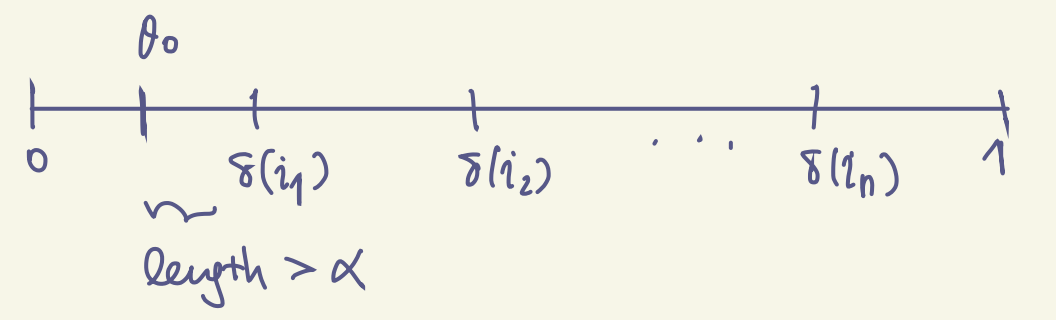
\includegraphics[width=0.7\textwidth]{figures/0-1loss.png}
    \caption{TO BE NAMED}
    \label{fig:01loss}
\end{figure}

\subsection{Admissibility of Minimax Estimator}

\begin{enumerate}
    \item Admissibility can give rise to minimaxity: 
    If $\delta$ is admissible with constant risk, 
    then $\delta$ is also minimax.
    \item Minimaxity does not guarantee admissibility: 
    It only ensures that the worst case risk is optimal\footnote{Recall Theorem \ref{thm:uniqbayesadm}, i.e. TPE 5.2.4.}.
\end{enumerate}

\begin{example}
    Let $X_1,\cdots,X_n\overset{iid}{\sim}\mathcal{N}(\theta,\sigma^2)$ with $\sigma^2$ known, 
    and $\theta$ is the estimated.
    Then the minimax estimator in $\Bar{X}_n$ under the squared error loss and we would like to 
    determine whether or not $\Bar{X}_n$ is admissible.

    \textbf{Question:} Let's try to answer a more general question: When is $a\Bar{X}_n+b$,
    for $a,b\in\mathbb{R}$ (i.e. affine function of $\Bar{X}_n$) admissible?
    \begin{enumerate}[{Case} 1]
        \item $0<a<1$:\\
        In this case $a\Bar{X}_n+b$ is a convex combination of $\Bar{X}_n$ and $b$.
        Bay our previous result,
        it is a Bayes estimator w.r.t. some Gaussian prior $\theta$.
        Since we adopt the squared error loss function,
        which is strictly convex,
        the Bayes estimator is unique.
        By Theorem \ref{thm:uniqbayesadm} (TPE 5.2.4, a unique Bayes estimator is always admissible),
        $a\Bar{X}_n+b$ is admissible.
        
        \item $a=0$:\\
        In this case $b$ is also a unique Bayes estimator w.r.t. 
        a degenerate prior distribution with the unique value at $\theta=b$,
        then by Theorem \ref{thm:uniqbayesadm}, b is also admissible.
        
        \item $a=1,b\neq{0}$:\\
        In this case $\Bar{X}_n+b$ is not admissible
        because it is dominated by $\Bar{X}_n$.
        Note that $\Bar{X}_n+b$ and $\Bar{X}_n$ have the same variance,
        but $\Bar{X}_n$ has a strictly smaller bias.
        
        \item $a>1$:\\
        In general, the risk of $a\Bar{X}_n+b$ is
        \begin{align}
            \mathbb{E}[a\Bar{X}_n+b-\theta]^2
            =& \mathbb{E}[a(\Bar{X}_n-\theta)+b+\theta(a-1)]^2\\
            =& \frac{a^2\sigma^2}{n} + [b+\theta(a-1)]^2\label{eq:caseadmiss}
        \end{align}
        In the case of $a>1$, by Equation \ref{eq:caseadmiss}, we have 
        \begin{gather}
            \mathbb{E}[a\Bar{X}_n+b-\theta]^2\geq\frac{a^2\sigma^2}{n}>\frac{\sigma^2}{n}=R(\theta,\Bar{X}_n)
        \end{gather}

        Hence, we conclude that $\Bar{X}_n$ dominates $a\Bar{X}_n+b$ 
        when $a>1$ in which case $a\Bar{X}_n+b$ is inadmissible.

        \item $a<0$:\\
        We have 
        \begin{align}
            \mathbb{E}[a\Bar{X}_n+b-\theta]^2
            >& [b-\theta(a-1)]^2\\
            =& (a-1)^2\left[\theta+\frac{b}{a-1}\right]^2\\
            >& \left[\theta-\left(-\frac{b}{a-1}\right)\right]^2
        \end{align}
        which is the risk of predicting with the constant $-\frac{b}{a-1}$.
        So, $-\frac{b}{a-1}$ dominates $a\Bar{X}_n+b$ and therefore $a\Bar{X}_n+b$ is again inadmissible.

        \item $a=1,b=0$:\\
        We shall proceed with a limiting Bayes argument.
        Suppose $\Bar{X}_n$ is inadmissible, then, WLOG,
        we let $\sigma^2=1$, we have $R(\theta,\Bar{X}_n)=\frac{1}{n}$.

        By our hypothesis, there must exist an estimator $\delta'$ such that
        $R(\theta,\delta')\leq\frac{1}{n}$ for all $\theta$ and 
        $R(\theta',\delta')<\frac{1}{n}$ for at least one $\theta'\in\Omega$.
        Because $R(\theta,\delta)$ is continuous in $\theta$, 
        there must exist $\varepsilon>0$ and an interval $(\theta_0,\theta_1)$ containing $\theta'$ such that
        \begin{gather}
            R(\theta,\delta')<\frac{1}{n}-\varepsilon~\forall{\theta}\in(\theta_0,\theta_1)\label{eq:caseadmiss2}
        \end{gather}

        Let $r'_\tau$ be the average risk of $\delta'$ w.r.t. the prior distribution $\mathcal{N}(0,\tau^2)$ on $\theta$.
        (We used the same prior to prove that $\Bar{X}_n$ was the limit of a Bayes estimator,
        and hence minimax.
        We did this by letting $\tau\to\infty$ (improper prior: $\pi(\theta)=1~\forall{\theta}$))
        Let $r_\tau$ be the average risk of a Bayes estimator $\delta_\tau$ under the same prior.
        Note that $\delta_\tau\neq\delta'$ because $R(\theta,\delta_\tau)\to\infty$ as $\theta\to\infty$,
        which is not consistent with $R(\theta,\delta')\leq\frac{1}{n}~\forall{\theta}\in\mathbb{R}$.
        So $r_\tau<r_\tau'$ because the Bayes estimator is unique almost surely w.r.t the marginal distribution of $\theta$.

        We shall look into the following ratio,
        which we shall show to become arbitrarily large and form a contradiction that $r_\tau<r_\tau'$.
        Using the form of the Bayes risk $r_\tau$, we can write
        \begin{gather}
            \frac{\frac{1}{n}-r_\tau'}
            {\frac{1}{n}-r_\tau}
            =
            \frac{\frac{1}{\sqrt{2\pi}\tau}
            \int_{-\infty}^\infty{
                \left[\frac{1}{n}-R(\theta,\delta')\right]\exp\left(-\frac{\theta^2}{2\tau^2}\right)
            }d\theta}
            {\frac{1}{n}-\frac{1}{n+1/\tau^2}}
        \end{gather}
        Applying Equation (\ref{eq:caseadmiss2}), we find:
        \begin{align}
            \frac{\frac{1}{n}-r_\tau'}{\frac{1}{n}-r_\tau}
            \geq& \frac{\frac{1}{\sqrt{2\pi}\tau}\int_{\theta_0}^{\theta_1}{
                \varepsilon\exp\left(-\frac{\theta^2}{2\tau^2}\right)
            }d\theta}
            {\frac{1}{n(n\tau^2+1)}}\\
            =& \frac{n(1+n\tau^2)\varepsilon}{\sqrt{2\pi}\tau}\int_{\theta_0}^{\theta_1}{
                \exp\left(-\frac{\theta^2}{2\tau^2}\right)
            }d\theta
        \end{align}
        As $\tau\to\infty$, the first expression $\frac{n(1+n\tau^2)\varepsilon}{\sqrt{2\pi}\tau}\to\infty$
        and since the integral converges monotonically to 1, 
        Lebesgue's MCT ensure that the integral approaches the positive quality $\theta_1-\theta_0$.
        So, for sufficiently large $\tau$, we must have 
        \begin{gather}
            \frac{\frac{1}{n}-r_\tau'}{\frac{1}{n}-r_\tau}
            > 1
            \iff 
            r_\tau'<r_\tau
        \end{gather}
        However this is a contradiction because $r_\tau$ is the optimal average risk
        since it is the Bayes risk.
        So our assumption that there was a dominating estimator $\delta$ is wrong
        and in this case $a\Bar{X}_n+b=\Bar{X}_n$ is admissible.
    \end{enumerate}
\end{example}

\subsection{Simultaneous Estimation}

So far, we consider only one parameter.

\begin{example}
    Let $X_1,\cdots,X_p$ be independent with $X_i\sim\mathcal{N}(\theta_i,\sigma^2)$
    for $1\leq{i}\leq{p}$.
    For the sake for simplicity, let $\sigma^2=1$.
    Our goal is to estimate $\boldsymbol{\theta}=(\theta_1,\cdots,\theta_p)^T$
    under the loss function 
    $L(\boldsymbol{\theta},\boldsymbol{d})=\sum_{i=1}^p(d_i-\theta_i)^2$.
    A natural estimator for $\boldsymbol{\theta}$ is $\boldsymbol{X}=(X_1,\cdots,X_p)^T$.
    It can be shown that $\boldsymbol{X}$ is the UMRUE,
    the MLE, a generalized Bayes and a minimax estimator for $\theta$.
    So it would be natural for us to think that $\boldsymbol{X}$ is admissible.
    However, it turns out that this is not the case when $p\geq{3}$.

    When $p\geq 3$, $\boldsymbol{X}$ is dominated by the James-Stein (J-S) estimator:
    \begin{gather}
        \delta(\boldsymbol{X})=(\delta_1(\boldsymbol{X}),\cdots,\delta_p(\boldsymbol{X}))
    \end{gather}
    where $\delta_i(\boldsymbol{X})=\left(1-\frac{p-2}{\|\boldsymbol{X}\|_2^2}\right)X_i$.
\end{example}
$~$\newline

Motivation for the J-S estimator (view it from the empirical Bayes framework):
\begin{enumerate}
    \item Suppose $\theta_i\overset{iid}{\sim}\mathcal{N}(0,A)$,
    then the Bayes estimator for $\theta_i$ is 
    \begin{gather}
        \delta_{A,i}(\boldsymbol{X})=\frac{X_i}{1+1/A}=\left(1-\frac{1}{A+1}\right)X_i
    \end{gather}
    \item We need to choose $A$:
    Marginalizing over $\theta$, we can show that $\boldsymbol{X}$ has the distribution
    \begin{gather}
        X_i\overset{iid}{\sim}\mathcal{N}(0,A+1)
    \end{gather}
    We may use $\boldsymbol{X}$ and the knowledge of this marginal distribution to find an estimate of $\frac{1}{A+1}$.
    Instead of using the M1E, we shall use an unbiased estimate.
    Considering that it can be shown that 
    \begin{gather}
        \mathbb{E}\frac{1}{\|\boldsymbol{X}\|_2^2}=\frac{1}{(p-2)(A+1)},~~~\left(\frac{\|\boldsymbol{X}\|_2^2}{A+1}\sim\chi^2_p\right)
    \end{gather}
    so $1-\frac{p-2}{\|\boldsymbol{X}\|_2^2}$ is UMVU for $1-\frac{1}{A+1}$.
\end{enumerate}

\begin{note}
    Note that
    \begin{align}
        \mathbb{E}\|\boldsymbol{X}\|_2^2
        =& \mathbb{E}\sum_{i=1}^pX_i^2
        = p + \sum_{i=1}^n{\theta_i^2}\\
        =& p + \|\boldsymbol{\theta}\|_2^2 > p.
    \end{align}
    $\Rightarrow$ We may view the J-S estimator as a method 
    for correcting the bias in the size of $\boldsymbol{X}$.\footnote{TPE 5.5.1 \& Keener 11.2}
\end{note}

\newpage
  \lesson{original Lecture 10 -- 12}{Hypothesis Testing}

\subsection{Model Setup}

We assume that the data are sampled from $X\sim{p_\theta}$,
where $p_\theta\in\mathcal{P}=\{p_\theta:\theta\Omega\}$.
We divide the models in $\mathcal{P}$ into two disjoint sub-classes known as hypothesis:
\begin{align}
    H_0:&~\theta\in\Omega_0\subset{\Omega}~\text{(null hypothesis)}\\
    H_1:&~\theta\in\Omega_1=\Omega\setminus\Omega_0~\text{(alternative hypothesis)}
\end{align}

Our goal is to infer (from the data) which hypothesis is ``correct''.
Our decision space is $\mathcal{D}=\{\text{accept}~H_0,~\text{reject}~H_1\}$.
The loss function of testing is shown as the confusion matrix Table \ref{tab:testconfmtx},
where $\beta$ is power.

% Table generated by Excel2LaTeX from sheet 'Sheet1'
\begin{table}[htbp]
  \centering
  \caption{Confusion matrix of testing's loss function $L(\theta,d)$}
    \begin{tabular}{cc|cc}
          &       & \multicolumn{2}{c}{Truth} \\
          &       & $\theta\in\Omega_0$ ($H_0$ is true) & $\theta\in\Omega_1$ ($H_0$ is false) \\
    \midrule
    \multirow{2}[1]{*}{Decision}
          & Reject $H_0$ & $\alpha$ (Type I error) & 0 \\
          & Accept $H_0$ & 0     & $1-\beta$ (Type II error) \\
    \end{tabular}
  \label{tab:testconfmtx}%
\end{table}%

We make decision with testing function (or critical function) $\varphi(X)\in[0,1]$,
which indicates that $\delta_\varphi(X,U)$ rejects $H_0$ with probability $\varphi(X)$, i.e.
\begin{gather}
    \varphi(X)=P(\delta_\varphi(X,U)=\text{Reject}~H_0|X)
\end{gather}
where $U\vperp X$ is randomized component.

\begin{definition}[Power function]
    The power function of a test $\varphi$ is 
    \begin{gather}
        \beta(\theta)=\mathbb{E}_\theta\varphi(X)=P_\theta(\text{Reject}~H_0)
    \end{gather}
    If $\theta\in\Omega_0$, then $\beta(\theta)=R(\theta,\delta_\varphi)=\text{Type I error}~(\alpha);$\\
    If $\theta\in\Omega_1$, then $\beta(\theta)=1-R(\theta,\delta_\varphi)=1-\text{Type II error}$.
\end{definition}

Our ideal goal is to minimize $\beta(\theta_0)$ uniformly for all $\theta\in\Omega_0$
and maximize $\beta(\theta)$ uniformly for all $\theta\in\Omega_1$.

\subsection{Neyman-Pearson Paradigm}

Fix $\alpha\in(0,1)$ to control the Type I error. (level of significance)
We require that all procedure can satisfy the following risk bound:
\begin{align}
    \sup_{\theta\in\Omega_0}\mathbb{E}_\theta\varphi(X) 
    = \sup_{\theta\in\Omega_0}\beta(\theta)\leq\alpha.
\end{align}
And our optimality goal is to find a level $\alpha$ test that maximises the power
$\beta(\theta)=\mathbb{E}_\theta\varphi(X)$ for each $\theta\in\Omega_1$.
Such a test is called uniformly most powerful test (UMP).

\subsection{Simple vs Simple}

MP test for the ``Simple vs Simple'' case.

\begin{definition}[Simple vs simple]
    A hypothesis $H_0$ is called simple if $|\Omega_0|=1$,
    otherwise it is called composite.
    The same is the for $H_1$.
\end{definition}


For the simple versus simple case, will adopt the notation:
\begin{align}
    H_0:&~X\sim{p_0}~~~(\theta=\theta_0)\\
    H_1:&~X\sim{p_1}~~~(\theta=\theta_1)
\end{align}
Our goal can be compactly described as following with predefined $\alpha$:
\begin{gather}
    \max_\varphi\mathbb{E}_{p_1}\varphi(X)\\
    \text{s.t.}~\mathbb{E}_{p_0}\varphi(X)\leq{\alpha}
\end{gather}

\begin{lemma}\label{lem:nplemma}
    \textbf{Neyman-Pearson Lemma}\\
    \begin{enumerate}[{(i)}]
        \item \textbf{Existence}\\
        For testing $H_0:p_0$ vs $H_1:p_1$,
        there is a test $\varphi(X)$ and a constant $k$ such that
        \begin{enumerate}[{a)}]
            \item $\mathbb{E}_{p_0}\varphi(X)=\alpha$ (size$=$level)
            \item $\varphi(x)=\left\{\begin{array}{ll}
                1 & \text{if}~\frac{p_1(x)}{p_0(x)}>k_\alpha \\
                0 & \text{if}~\frac{p_1(x)}{p_0(x)}<k_\alpha
            \end{array}\right.$,
            where $\frac{p_1(x)}{p_0(x)}>k_\alpha$ is rejection (or critical) region, 
            i.e. rejecting $H_0$ if $\frac{p_1(x)}{p_0(x)}>k_\alpha$.
            This test is called a \textbf{likelihood ratio test}.
        \end{enumerate}
        \item \textbf{Sufficiency}\\
        If a test statistics (a) and (b) for some constant $k_\alpha$,
        it is most powerful for testing $H_0:p_0$ vs $H_1:p_1$ at level $\alpha$.
        \textbf{$\varphi$ is MP.}
        \item \textbf{Necessity}\\
        If a test $\varphi$ is MP at level $\alpha$,
        then it satisfies (b) for some $k_\alpha$ and it also satisfies (a)
        unless there exists a test of size $<\alpha$ with power $1$.
    \end{enumerate}
\end{lemma}
\begin{proof}
    skipped, refer to (Keener, 2010) if it is needed.
\end{proof}

\begin{example}
    Let $X_1,\cdots,X_n\overset{iid}{\sim}\mathcal{N}(\mu,\sigma^2)$ with $\sigma^2$ known.
    Consider the two hypotheses: $H_0:\mu=0$ vs $H_1:\mu=\mu_1$ ($\mu_1>0$ known).
    \begin{align}
        L(\boldsymbol{x})
        =& \frac{p_1(\boldsymbol{x})}{p_0(\boldsymbol{x})}
        = \frac{\prod_{i=1}^n\frac{1}{\sqrt{2\pi\sigma^2}}\exp\left\{-\frac{(x_i-\mu_1)^2}{2\sigma^2}\right\}}
        {\prod_{i=1}^n\frac{1}{\sqrt{2\pi\sigma^2}}\exp\left\{-\frac{x_i^2}{2\sigma^2}\right\}}\\
        =& \exp\left\{\frac{\mu_1}{\sigma^2}{\sum_{i=1}^n{x_i}}-\frac{n\mu_1^2}{2\sigma^2}\right\}
    \end{align}
    We have the following observeation:
    \begin{align}
        L(\boldsymbol{x})>k
        \Rightarrow& \frac{\mu_1}{\sigma^2}{\sum_{i=1}^n{x_i}}-\frac{n\mu_1^2}{2\sigma^2}>\log{k}\\
        \Rightarrow& \mu_1\sum_{i=1}^n{x_i}>k'\\
        \Rightarrow& \left\{\begin{array}{ll}
            \sum_{i=1}^n{x_i}>k'' & \text{if}~\mu_1>0 \\
            \sum_{i=1}^n{x_i}<k'' & \text{if}~\mu_1<0
        \end{array}\right.
    \end{align}
    Let's focus on the first case when $\mu_1>0$.
    We can rewrite our test in a different form as follows:
    \begin{gather}
        \frac{\sqrt{n}\Bar{x}_n}{\sigma}>k'''.
    \end{gather}
    By NP Lemma, we reject $H_0$ if and only if $\frac{\sqrt{n}\Bar{x}_n}{\sigma}>k_\alpha$ is MP,
    where $k'''=k(\alpha)=z_{1-\alpha}$ is the $1-\alpha$ quantitle of $\mathcal{N}(0,1)$.
\end{example}


\begin{definition}[Power of testing]
    For simple $H_0:p_0$ vs $H_1:p_1$,
    we call $\beta_\varphi(p_1)=\mathbb{E}_{p_1}\varphi(X)$ the power of $\varphi$,
    i.e. the probability of rejecting $H_0$ under the alternative hypothesis.
\end{definition}

\begin{corollary}
    Suppose $\beta$ is the power of a most powerful level $\alpha$ test of $H_0:p_0$ vs $H_1:p_1$ with $\alpha\in[0,1)$,
    then $\alpha<\beta$ unless $p_0=p_1$.\footnote{TSH 3.2.1}
    That is saying this MP test rejects more often under $H_1$ then $H_0$.
\end{corollary}
\begin{proof}
    Consider the test $\varphi_0(X)\equiv\alpha$, 
    which always rejects with probability $\alpha$.
    Since $\varphi_0$ is level $\alpha$ and $\beta$ is the maximal pwer, we have
    \begin{gather}
        \beta\geq\mathbb{E}_{p_1}\varphi_0(X)=\alpha.
    \end{gather}
    Suppose $\beta=\alpha$, then $\varphi_0(X)=\alpha$ is a most powerful level $\alpha$ text.
    As a result, by Lemma \ref{lem:nplemma}, NP Lemma, (iii),
    \begin{gather}
        \varphi_0(x)=\left\{\begin{array}{ll}
            1 & \text{if}~\frac{p_1(x)}{p_0(x)}>k, \\
            0 & \text{if}~\frac{p_1(x)}{p_0(x)}<k.
        \end{array}\right.
    \end{gather}
    Since $\varphi_0(X)$ never equals 0 or 1, 
    it must be the case that $p_1(x)=kp_0(x)$ with probability 1.
    Note that 
    \begin{gather}
        \int{p_1(x)}d\mu(x)=k\int{p_0}d\mu(x)=1,
    \end{gather}
    which implies that $k=1$, and hence $p_0=p_1$.
\end{proof}

\subsection{Exponential Families and UMP One-side Tests}

\textbf{Goal}: Extend the MP tests for simple alternatives up to 
\textbf{uniformly most powerful} (UMP) tests for composite alternatives.

\begin{example}
    \textbf{One-parameter exponential family}\\
    Consider $X_1,\cdots,X_n\overset{iid}{\sim}p_\theta$,
    where $p_\theta(x)\propto h(x)\exp\{\theta{T(x)}\}$,
    and we are interested in testing 
    \begin{gather}
        H_0:\theta=\theta_0~ \text{vs} ~H_1:\theta=\theta_1
    \end{gather}.
    We want to construct an MP test at level $\alpha$.
    The corresponding likelihood ratio is 
    \begin{gather}
        \frac{\prod_{i=1}^n p_{\theta_1}(x_i)}{\prod_{i=1}^n p_{\theta_0}(x_i)}
        \propto
        \exp\left\{
            (\theta_1-\theta_0)\sum_{i=1}^n{T(x_i)}
        \right\}
    \end{gather}
    Assuming that $\theta_1>\theta_0$,
    we shall reject for large value of $\sum_{i=1}^n T(x_i)$.
    That is, an MP test has the following form:
    \begin{gather}
    \varphi(\boldsymbol{x})=\left\{\begin{array}{ll}
        1       & \text{if}~\sum_{i=1}^n{T(x_i)}>k, \\
        \gamma  & \text{if}~\sum_{i=1}^n{T(x_i)}=k, \\
        0       & \text{if}~\sum_{i=1}^n{T(x_i)}<k,
    \end{array}\right.
    \end{gather}
    where $k$ and $\gamma$ are chosen to satisfy the size constraint:
    \begin{align}
        \alpha=\mathbb{E}_{\theta_0}\varphi(X)
        = P_{\theta_0}\left(\sum_{i=1}^n T(X_i)>k\right)
        + \gamma P_{\theta_0}\left(\sum_{i=1}^n T(X_i)>k\right).
    \end{align}

    Note that $\sum_{i=1}^n T(X_i)$ has no explicit $\theta$ dependence
    and that $k$ and $\gamma$ do not depend on $\theta_1$ (with $\theta_1>\theta_0$).
    This means that $\varphi$ is in fact a UMP test for testing 
    \begin{gather}
        H_0:\theta=\theta_0~ \text{vs} ~H_1:\theta>\theta_0
    \end{gather}.
    Hence $H_1$ is an example of a one-sided alternative,
    which arises when the parameter values of interest lie on only one side of the real-valued parameter $\theta_0$.
\end{example}

\begin{definition}
    \textbf{Families with monotone likelihood ratio (MLR)}\\
    We say that the family of densities $\{p_\theta:\theta\in\mathbb{R}\}$ has monotone likelihood ratio inn $T(X)$ if
    \begin{enumerate}[{(1)}]
        \item $\theta\neq\theta'$ implies $p_{\theta}\neq p_{\theta'}$ (identifiability),
        \item $\theta<\theta'$ implies $\frac{p_{\theta'(x)}}{p_{\theta}(x)}$ is a non-decreasing function of $T(X)$ (monotonicity).
    \end{enumerate}
\end{definition}

\begin{example}
    $~$\\
    \begin{enumerate}[{1)}]
        \item $T(\boldsymbol{X})=\sum_{i=1}^n T(X_i)$ in the one-parameter exponential family.
        \item (Double exponential) Let $X\sim\text{DExp}(\theta)$ with density
        $p_\theta(x)=\frac{1}{2}\exp\{-|x-\theta|\}$.
        It is easy to see that the model is identifiable,
        so we need check only the condition (ii) in the definition of MLR.

        Fix any $\theta'>\theta$, and consider the likelihood ratio
        \begin{gather}
            \frac{p_{\theta'(x)}}{p_\theta(x)}
            =\exp\{|x-\theta|-|x-\theta'|\}.
        \end{gather}
        Note that 
        \begin{gather}
            |x-\theta|-|x-\theta'|=\left\{\begin{array}{cc}
                \theta-\theta'      & \text{if}~x<\theta \\
                2x-\theta-\theta'   & \text{if}~\theta\leq{x}\leq\theta \\
                \theta'-\theta      & \text{if}~x>\theta
            \end{array}\right.
        \end{gather}
        which is non-decreasing in $x$.
        Therefore, the family has MLR in $T(X)=X$.
    \end{enumerate}
\end{example}

\begin{example}
    \textbf{Cauchy location model}\\
    Let $X$ has density 
    \begin{gather}
        p_\theta=\frac{1}{\pi}\cdot\frac{1}{1+(x-\theta)^2}.
    \end{gather}
    We find two points for which the MLR conditions fails:
    For any fixed $\theta>0$,
    \begin{gather}
        \frac{p_\theta(x)}{p_0(x)}=\frac{1+x^2}{1+(x-\theta)^2}\to{1}~\text{as}~x\to\pm\infty.
    \end{gather}
    But $\frac{p_\theta(0)}{p_0(0)}=\frac{1}{1+\theta^2}<1$.
    Thus the ratio must increase at some values of $x$ and decrease at others.
    In particular, it is not monotone in $x$.
    Hence, we can conclude that the LR in $T(X)=X$ is not MLR.
\end{example}

\begin{theorem}
    Suppose $X\sim p_\theta$ has MLR in $T(X)$ and we test
    \begin{gather}
        H_0:\theta\leq\theta_0~\text{vs}~H_1:\theta>\theta_0,
    \end{gather}
    then\footnote{
    TSH 3.4.1
    }
    \begin{enumerate}[{(i)}]
        \item There exists a UMP test at level $\alpha$ of the form
        \begin{gather}
            \varphi(X)=\left\{\begin{array}{ll}
                1 & \text{if}~T(X)>k \\
                \gamma & \text{if}~T(X)=k \\
                0 & \text{if}~T(X)<k 
            \end{array}\right.
        \end{gather}
        where $k,\gamma$ are determined by the condition $\mathbb{E}_{\theta_0}\varphi(X)=\alpha$.
        \item The power function $\beta(\theta)=\mathbb{E}_\theta\varphi(X)$ is strictly increasing when $0<\beta(\theta)<1$.
    \end{enumerate}
\end{theorem}
\begin{proof}
    refer to TSH
\end{proof}

\begin{note}
    Possible directions for constructing UMPs:
    \begin{enumerate}
        \item Reduce the composite alternative to a simple alternative
        \item Collapse the composite null to simple null
        \item Apply NP Lemma.
    \end{enumerate}
\end{note}

\subsection{Optimal Tests for Composite Nulls}

\begin{gather}\begin{array}{ll}
    H_0:X\sim f_\theta & \theta\in\Omega_0 \\
    H_1:X\sim g & g~\text{unknown}
\end{array}\end{gather}
We may impose a prior distribution $\Lambda$ on $\Omega_0$.
So, we consider the new hypothesis converting composite null to simple one:
\begin{gather}
    H_\Lambda:X\sim h_\Lambda(x)=\int_{\Omega_0}f_\theta(x)d\Lambda(\theta)
\end{gather}
where $h_\lambda(x)$ is the marginal distribution of $X$ induced by $\Lambda$.
Let $\beta_\Lambda$ be the power of the MP level-$\alpha$ test $\varphi_\Lambda$ for testing $H_\Lambda$ vs $g$.\footnote{
TSH 3.8
}

\begin{definition}
    \textbf{Least favourable distribution}\\
    $\Lambda$ is a least favourable distribution if $\beta_\Lambda\leq\beta_{\Lambda'}$ for any prior $\Lambda'$.
\end{definition}

\begin{theorem}\label{thm:convertcompsim}
    Suppose $\varphi_\Lambda$ is an MP level-$\alpha$ test for testing $H_\Lambda$ against g.
    If $\varphi_\Lambda$ is level-$\alpha$ for the original hypothesis $H_0$
    (i.e. $\mathbb{E}_{\theta_0}\varphi_\Lambda\leq\alpha~\forall\theta_0\in\Omega$), then\footnote{
    TSH 3.8.1
    }
    \begin{enumerate}[{(i)}]
        \item the test $\varphi_\Lambda$ is MP for the original test on $H_0:\theta\in\Omega_0$ vs $g$ and 
        \item the prior distribution $\Lambda$ is least favourable.
    \end{enumerate}
\end{theorem}
\begin{proof}
    $~$\\
    \begin{enumerate}[{(i)}]
        \item Let $\varphi^*$ be any other level-$\alpha$ test of $H_0:\theta\in\Omega$ vs $g$.
        Then $\varphi^*$ is also a level-$\alpha$ test for $H_\Lambda$ vs $g$
        because
        \begin{gather}
            \mathbb{E}_\theta\varphi^*(X)=\int{\varphi^*(x)f_\theta(x)}d\mu(x)\leq\alpha~~~\forall{\theta}\in\Omega_0
        \end{gather}
        which implies that 
        \begin{gather}
            \int{\varphi^*(x)h_\Lambda(X)}d\mu(x)
            = \iint\varphi^*(x)f_\theta(x)d\mu(x)d\Lambda(\theta)
            \leq \int{\alpha}d\Lambda(\theta)
            =\alpha
        \end{gather}
        Since $\varphi_\Lambda$ is MP for $H_\Lambda$ vs $g$, we have 
        \begin{gather}
            \int\varphi^*g(x)d\mu(x)\leq\int{\varphi_\Lambda(x)g(x)}d\mu(x)
        \end{gather}
        Hence $\varphi_\Lambda$ is a MP test for $H_0$ vs $g$ because $\varphi_\Lambda$ is also level $\alpha$.
        \item Let $\Lambda'$ be any distribution on $\Omega_0$.
        Since $\mathbb{E}_\theta\varphi_\Lambda(X)\leq\alpha~\forall\theta\in\Omega_0$,
        we know that $\varphi_\Lambda$ must be level $\alpha$ for $H_\Lambda'$ vs $g$.
        Thus $\beta_\Lambda\leq\beta_{\Lambda'}$.
        So $\Lambda$ is the least favorable distribution.
    \end{enumerate}
\end{proof}

\begin{example}
    \textbf{Testing in the presence of nuisance parameters}\\
    Let $X_1,\cdots,X_n\overset{iid}{\sim}\mathcal{N}(\theta,\sigma^2)$
    where both $\theta$ and $\sigma^2$ are unknown.
    We consider testing $H_0:\sigma\leq\sigma_0$ against $H_1:\sigma>\sigma_0$.
    To find a UMP test,
    we follow the strategy discussed in the previous lecture:
    \begin{enumerate}
        \item First, we fix a simple alternative ($\theta_1,\sigma_1$) for some arbutrary $\theta_1$ and $\sigma_1>\sigma_0$.
        \item We choose a prior distribution $\Lambda$ to collapse our null hypothesis over.
        Intuitively, the least favourable prior should make the alternative hypothesis hard to distinguish.
        One Sensible choice is concentrating $\Lambda$ on the boundary between $H_1$ and $H_0$
        (i.e. the limit $\{\sigma=\sigma_0\}$ ???).
        Thus $\Lambda$ will be a probability distribution over $\theta\in\mathbb{R}$ for the fixed $\sigma=\sigma_0$.
        
        Given any test function $\varphi(X)$ and a sufficient statistic $T$,
        thus exists a test function $\eta$ that has the same power as $\varphi$,
        but depends on $x$ only through $T$:
        \begin{gather}
            \eta(T(X))=\mathbb{E}[\varphi(X)|T(X)].
        \end{gather}

        Hence, we can restrict our attention to the sufficient Statistic $(Y,U)$,
        where $Y=\Bar{X}_n$ and $U=\sum_{i=1}^n(X_i-\Bar{X}_n)^2$.
        We know that $Y\sim\mathcal{N}(\theta,\frac{\sigma^2}{n})$,
        $U\sim\sigma^2\chi^2_{n-1}$ and $Y$ is independent of $U$ by Basu's Theorem.

        Thus, for $\Lambda$ supported on $\sigma=\sigma_0$,
        we have he joint density of $(Y,U)$ under $H_\Lambda$ as 
        \begin{gather}
            c_0 u^\frac{n-3}{2} \exp\left( -\frac{u}{2\sigma_0^2} \right)
            \int\exp\left\{ -\frac{u}{2\sigma_0^2}(y-u)^2 \right\}d\Lambda(\theta) \label{eq:comph01}
        \end{gather}
        and the joint density under the alternative hypothesis $(\theta,\sigma_1)$ as 
        \begin{gather}
            c_0 u^\frac{n-3}{2} \exp\left( -\frac{u}{2\sigma_1^2} \right)
            \exp\left\{ -\frac{n}{2\sigma_1^2}(y-\theta_1)^2 \right\}\label{eq:comph02}
        \end{gather}
        
        We see from Equations (\ref{eq:comph01}) and (\ref{eq:comph02}) 
        that the choice of $\Lambda$ only affects the distribution of $Y$.
        To achieve the maximum power against the alternative,
        we need to choose $\Lambda$ such that 
        the two distributions become as close as possible under $H_1:Y\sim\mathcal{N}(\theta,\frac{\sigma_1}{n})$.
        Under $H_1$, the distribution of $Y$ is in a convolution form:
        $Y=Z+\Theta$ for $Z\sim\mathcal{0,\frac{\sigma_0^2}{n}}$ and $\Theta\sim \Lambda$,
        where $\Theta$ and $Z$ are independent.
        Hence, if we choose $\Theta\sim\mathcal{N}(\theta_1,\frac{\sigma_1^2-\sigma_0^2}{n})$,
        $Y$ will have the same distribution under the null and the alternative,
        which is $\mathcal{N}(\theta_1,\frac{\sigma_1^2}{n})$.
        Under this choice of prior,
        the LRT rejects for large values of $\exp\left\{-\frac{u}{s\sigma_1^2}+\frac{u}{2\sigma_0^2}\right\}$,
        i.e. it rejects for large values of $u$ since $\sigma_1>\sigma_0$.
        So, the MP test rejects $H_\Lambda$ 
        if $\sum_{i=1}^n(X_i-\Bar{X}_n^2)$ lies above some threshold determined by the size constraint.
        In particular, it rejects if $\sum_{i=1}^n(X_i-\Bar{X}_n^2)>\sigma_0^2c_{n-1,1-\alpha}$,
        where $c_{n-1,1-\alpha}$ is the $(1-\alpha)$-th quantile of $\chi^2_{n-1}$.

        \item Next, we check if the MP test is level $\alpha$ for the composite null.
        For any $(\theta,\sigma)$ with $\sigma\leq\sigma_0$, the probability of rejection is 
        {\footnotesize\begin{gather}
            P_{\theta,\sigma}\left( 
                \frac{\sum_{i=1}^n(X_i-\Bar{X}_n)^2}{\sigma^2}
                > \frac{\sigma_0^2 c_{n-1,1-\alpha}}{\sigma^2} 
            \right)
            = P\left(
                \chi_{n-1}^2
                > \frac{\sigma_0^2}{\sigma^2} c_{n-1,1-\alpha}
            \right)
            \leq \alpha
        \end{gather}}
        where the equality holds if and only if $\sigma=\sigma_0$.
        Hence from Theorem \ref{thm:convertcompsim} (TSH 3.8.1) that our test is MP for testing the
        original null $H_0$ vs $\mathcal{N}(\theta_1,\sigma_1)$.
        \item Finally, the MP level-$\alpha$ test for testing 
        the composite null $H_0$ vs an arbitrarily chosen $(\theta_1,\sigma_1)$ does not depend on the choice of $(\theta_1,\sigma_1)$.
        Hence, it is UMP for testing the original composite null vs the composite alternatives.
    \end{enumerate}
\end{example}

\subsection{Duality between Testing and Interval Estimation}

\subsubsection{Confidence Interval}

Recall that a random set $S(X)$ is a $1-\alpha$ confidence region (or interval) 
for a parameter $\xi=\xi(\theta)$ if 
\begin{gather}
    P_\theta(\xi\in S(X))\geq 1-\alpha~~~\forall{\theta}\in\Omega
\end{gather}

For every $\xi_0$, let $A(\xi_0)$ be the acceptance region for non-randomized level-$\alpha$ test of 
$H_0:\xi(\theta)=\xi_0$ vs $H_1:\xi(\theta)\neq\xi_0$, so that 
\begin{gather}
    P_\theta(X\in A(\xi(\theta))) \geq 1-\alpha~~~\forall{\theta}\in\Omega.
\end{gather}
Define $S(x)=\{\xi:x\in A(\xi)\}$, then $\xi(\theta)\in S(X)$ if and only if $X\in A(\xi(\theta))$, so
\begin{gather}
    P_\theta(\xi(\theta)\in S(X))=P_\theta(X\in A(\xi(\theta)))\geq 1-\alpha.
\end{gather}
This shows that $S(X)$ is a $1-\alpha$ \textbf{confidence interval} (CI) for $\xi$.


\subsubsection{P-value}

For varying $\alpha$, the resulting tests provide an example of the typical situation
in which the rejection regions $S_\alpha$ are nested in the sense that 
\begin{gather}
    S_\alpha\subset S_{\alpha'}~\text{if}~\alpha<\alpha'.
\end{gather}
The quantity $\hat{p}=\hat{p}(X)=\inf\{\alpha:X\in S_\alpha\}$, 
the smallest significant level of observation, is called a p-value.
It gives an idea of how strongly the data contradict the null hypothesis.

\begin{example}
    Let $\Phi$ denote the standard normal cdf,
    then the rejection region can be written as 
    \begin{gather}
        S_\alpha
        = \{x:x>\sigma z_{1-\alpha}\}
        = \left\{x: \Phi(x/\sigma)>1-\alpha\right\}
        = \left\{x:1-\Phi(x/\sigma)<\alpha\right\}.
    \end{gather}
    For a given observed value of $X$, 
    the infimum over all $\alpha$ where the last inequality holds is $\hat{p}=1-\Phi(x/\sigma)$.

    Alternatively, the p-value is $p_0(X\geq x)$,
    where $x$ is the observed value of $X$.
    Note that under $\xi=0$, 
    the distribution of $\hat{p}$ is given by
    \begin{gather}
        P_0(\hat{p}\leq u)
        = P_0(1-\Phi(X/\sigma)\leq u)
        = P_0(\Phi(X/\sigma)\geq{1-u})=u
    \end{gather}
    $\Rightarrow\hat{p}$ is uniformly distributed on (0,1).\footnote{
    TSH Lemma 3.3.1 and Example 3.3.2
    }
\end{example}

\subsection{UMP}

\begin{enumerate}
    \item Impose a reasonable restriction on the tests to be considered 
    and the ``optimal'' tests within the class of tests under the restriction.
    \item Two typical strategies:
    \begin{enumerate}
        \item unbiasedness: UMP unbiased test
        \item invariance
    \end{enumerate}
\end{enumerate}

Recall that a UMP test $\varphi$ of size $\alpha$ has the property test 
\begin{gather}
    \mathbb{E}_\theta\varphi(X)\leq\alpha~\forall{\theta}\in\Omega_0
    ~\text{and}~
    \mathbb{E}_\theta\varphi(X)\geq\alpha~\forall{\theta}\in\Omega_1.
    \label{eq:ump}
\end{gather}
This means that $\varphi$ is at least as good as the naive test $\varphi\triangleq\alpha$.

\begin{definition}[Unbiased and Uniformly most powerful unbiased]
    Let $\alpha$ be a given level of significance. 
    A test $\varphi$ for $H_0:\theta\in\Omega_0$ vs $H_1:\theta\in\Omega_1$ is said to be \textbf{unbiased} of level $\alpha$,
    if and only if Equation (\ref{eq:ump}) holds.
    A test of size $\alpha$ is called a \textbf{uniformly most powerful unbiased} (UMPU) test,
    if and only if it is UMP within the class of unbiased tests of level $\alpha$.\footnote{
    Keener 12.7, Theorem 12.26 and Example 12.29.
    }
\end{definition}

More about \textbf{Consistency/Asymptotic Normality of MLE} referring to Keener Chapter 9 (EE, EM algorithms)







  % \input{lectures/lec06.tex}
  % \input{lectures/lec07.tex}
  % \input{lectures/lec08.tex}
  % \input{lectures/lec09.tex}
  % \input{lectures/lec10.tex}
  % \input{lectures/lec11.tex}
  % \input{lectures/lec12.tex}

  \listnotes
  \bibliography{ref}
\end{document}